\def\coursename{核辐射物理}
\def\coursefullname{核辐射物理及探测学}
\def\courseEnglishname{Nuclear Radiation Physics and Detection}
\def\teachername{杨祎罡}
\def\beginday{2022/9/30}

\documentclass[a4paper, 11pt]{article}

\usepackage[UTF8]{ctex}

\usepackage[T1]{fontenc}								% 字体
\catcode`\。=\active
\newcommand{。}{.} % {\ifmmode\text{.}\else .\fi}
\catcode`\(=\active
\catcode`\)=\active
\newcommand{(}{(}
\newcommand{)}{)}

% \usepackage{zhlineskip}

\usepackage{nicematrix}
% \usepackage{setspace}
% \linespread{1}						% 一倍行距
\setlength{\headheight}{14pt}			% 页眉高度
% \setlength{\lineskip}{0ex}			% 行距
\renewcommand\arraystretch{.82}		% 表格

\usepackage{amssymb, amsmath, amsfonts, amsthm}			% 数学符号,公式,字体,定理环境
\everymath{\displaystyle}			% \textstyle \scriptstyle \scriptscriptstyle
\allowdisplaybreaks[4]      		% 使用行间公式格式
% \makeatletter
% \renewcommand{\maketag@@@}[1]{\hbox{\m@th\normalsize\normalfont#1}}
% \makeatother
\newif\ifcontent\contenttrue		% if 显示目录
\newif\ifparskip\parskipfalse		% if 增加目录后的行距
\newif\ifshowemail\showemailfalse	% if 显示 email
\def\firstandforemost{
	\maketitle
	%\thispagestyle{empty}\clearpage
	\ifcontent
		\renewcommand{\contentsname}{目录}
		\tableofcontents
		\thispagestyle{empty}
		\clearpage
	\fi
	\ifparskip
		\setlength{\parskip}{.8ex}	% 设置额外的段距,目录后
	\fi								% 在 \firstandforemost 前设置 \parskiptrue
	\makenomenclature
	\printnomenclature
	\setcounter{page}{1}
}

\usepackage{mathtools}									% \rcase 环境等

% \usepackage{physics}

\usepackage[]{siunitx}									% 国际制单位
\sisetup{
	inter-unit-product = \ensuremath{{}\cdot{}},
	per-mode = symbol,
	per-mode = reciprocal-positive-first,
	range-units = single,
	separate-uncertainty = true,
	range-phrase = \ifmmode\text{\;-\;}\else\;-\;\fi
}
\DeclareSIUnit\angstrom{\text{Å}}
\DeclareSIUnit\atm{\text{atm}}
% SIunits 额外定义了一个 \square 表示平方,
% 还会把 \cdot 空格加大,真有够无语的 😅

\usepackage{authblk}									% 作者介绍
\ifx \coursefullname\undefined
	\ifx \coursename\undefined
		\def\coursename{笔记}
	\fi
	\def\coursefullname{\coursename}
\fi
\ifx \authorname\undefined
	\def\authorname{Dait}
\fi
\ifx \departmentname\undefined
	\def\departmentname{THU}
\fi
\ifx \emailaddress\undefined
	\def\emailaddress{daiyj20@mails.tsinghua.edu.cn}
\fi
\ifx \beginday\undefined
	\def\beginday{2021}
\fi
\ifx \endday\undefined
	\def\endday{\number\year/\number\month/\number\day}
\fi
\ifx \titleannotation\undefined
	\ifx \teachername\undefined
		\title{\textbf{\coursefullname}}
	\else
		\title{\textbf{\coursefullname}\\\small\textit{主要整理自\teachername 老师讲义}}
	\fi
\else
	\title{\textbf{\coursefullname}\\\small\textit{(\titleannotation)}}
\fi
\newif\ifdefaultauthor\defaultauthortrue
\ifdefaultauthor
	\author{by~\authorname~at~\departmentname}
	\ifshowemail
		\affil{\emailaddress}
	\fi
\fi
\ifx \endday\beginday
	\date{\beginday}
\else
	\date{\beginday~-~\endday}
\fi

\usepackage{hyperref}									% 链接
\ifx \courseEnglishname\undefined
	\def\courseEnglishname{Note}
\fi
\ifx \authorEnglishname\undefined
	\def\authorEnglishname{Dait}
\fi
\hypersetup{
	% dvipdfm								% 表示用 dvipdfm 生成 pdf
	pdftitle={\coursename},
	pdfauthor={\authorname},
	colorlinks=true, breaklinks=true,		% 超链接设置
	linkcolor=black, citecolor=black, urlcolor=blue
}

\usepackage[british]{babel}								% 长单词自动连字符换行
\hyphenation{long-sen-ten-ce}				% 自定义拆分方式

\usepackage{tikz}
\usetikzlibrary{quotes, angles}
\usepackage{pgfplots}
\pgfplotsset{compat=1.17}								% TikZ
\newcommand{\coor}[5][0]{
	\draw[thick,latex-latex](#1,#3)node[left]{$#5$}--(#1,0)node[shift={(-135:7pt)}]{$O$}--(#1+#2,0)node[right]{$#4$}
}			% 坐标轴

\usepackage{enumerate}									% 编号
\usepackage{paralist}
\setlength{\pltopsep}{1ex}
\setlength{\plitemsep}{1ex}
\ifx \eqnrange\undefined
	\numberwithin{equation}{section}
\else
	\numberwithin{equation}{\eqnrange}
\fi

\renewcommand{\thempfootnote}{\Roman{mpfootnote}}
\renewcommand{\thefootnote}{\Roman{footnote}}		% 注释上标 I, II,...
\newcommand{\sectionstar}[1]{
	\section[\hspace{-.8em}*\hspace{.3em}#1]{\hspace{-1em}*\hspace{.5em}#1}
}
\newcommand{\subsectionstar}[1]{					% 带星号的 section 和 subsection
	\subsection{\hspace{-1em}*\hspace{.5em}#1}
}
\newcommand{\subsubsectionstar}[1]{					% 带星号的 section 和 subsection
	\subsubsection{\hspace{-1em}*\hspace{.5em}#1}
}
\newcommand*{\appendiks}{
	\appendix
	\part*{附录}
	\addcontentsline{toc}{part}{附录}
}
\iffalse			% 不清楚
	\newcommand{\varsection}[1]{
		\refstepcounter{section}
		\section*{\thesection\quad #1}
		\addcontentsline{toc}{section}{\makebox[0pt][r]{*}\thesection\quad #1}
	}
\fi

\usepackage{fancyhdr}									% 页眉页脚
\ifx \coursename\undefined
	\def\coursename{笔记}
\fi
\fancyhf{}\pagestyle{fancy}
\fancyhead[L]{\coursename\rightmark}
\fancyhead[R]{by~\authorname}
\fancyfoot[C]{-~\thepage~-} 			%页码

\usepackage{colortbl, booktabs}							% 表

\usepackage{graphicx}
\usepackage{float}
\usepackage{caption}									% 图
\captionsetup{
	margin=20pt, format=hang,
	justification=justified
}
\newcounter{tikzpic}
\def\tikzchap{
	\stepcounter{tikzpic}\\
	\small 图~\thetikzpic\quad
}
\newcounter{linetable}
\newcommand{\tablechap}[1]{
	\stepcounter{linetable}
	{\small 表~\thelinetable\quad #1}\\[1em]
}

\usepackage{tcolorbox}									% 盒子
\tcbuselibrary{theorems, skins, breakable}
\definecolor{MatchaGreen}{HTML}{73C088}		% 抹茶绿B7C6B3
\newtcbtheorem[number within = subsection]{example}{例}{
	enhanced, breakable, sharp corners,
	attach boxed title to top left = {yshifttext = -1mm},
	before skip = 2ex,
	colback = MatchaGreen!5,				% 文本框内的底色
	colframe = MatchaGreen,					% 文本框框沿的颜色
	fonttitle = \bfseries,					% 标题字体用粗体	coltitle 默认 white,
	boxed title style = {
			sharp corners, size = small, colback = MatchaGreen,
		}
}{exm}
\definecolor{MelancholyBlue}{HTML}{9EAABA}	% melancholy: 沮丧
\newcounter{pslt}
\setcounter{pslt}{-1}
\newtcbtheorem[use counter = pslt]{posulate}{假设}{
	enhanced, breakable, sharp corners,
	attach boxed title to top left = {yshifttext = -1mm}, before skip = 2ex,
	colback = MelancholyBlue!5, colframe = MelancholyBlue, fonttitle = \bfseries,
	boxed title style = {
			sharp corners, size = small, colback = MelancholyBlue,
		}
}{psl}
\definecolor{PureBlue}{HTML}{80A3D0}
\newtcbtheorem[number within = subsection]{definition}{定义}{
	enhanced, breakable, sharp corners,
	attach boxed title to top left = {yshifttext = -1mm}, before skip = 2ex,
	colback = PureBlue!5, colframe = PureBlue, fonttitle = \bfseries,
	boxed title style = {
			sharp corners, size = small, colback = PureBlue,
		}
}{dfn}
\definecolor{PeachRed}{HTML}{EA868F}
\newtcbtheorem[number within = subsection]{theorem}{定理}{
	enhanced, breakable, sharp corners,
	attach boxed title to top left = {yshifttext = -1mm}, before skip = 2ex,
	colback = PeachRed!5, colframe = PeachRed, fonttitle = \bfseries,
	boxed title style = {
			sharp corners, size = small, colback = PeachRed,
		}
}{thm}
\definecolor{SchembriumYellow}{HTML}{fbd26a}	% 申博太阳城黄
\newtcbtheorem[number within = section]{method}{方法}{
	enhanced, breakable, sharp corners,
	attach boxed title to top left = {yshifttext = -1mm}, before skip = 2ex,
	colback = SchembriumYellow!5, colframe = SchembriumYellow, fonttitle = \bfseries,
	boxed title style = {
			sharp corners, size = small, colback = SchembriumYellow,
		}
}{mtd}
% 保留颜色
\definecolor{fadedgold}{HTML}{D9CBB0}		% 褪色金
\definecolor{saturatedgold}{HTML}{F0E0C2}	% staurated: 饱和
\definecolor{elegantblue}{HTML}{C4CCD7}		% elegant: 优雅
\definecolor{ivory}{HTML}{F1ECE6}			% 象牙
\definecolor{gloomypruple}{HTML}{CCC1D2}	% 阴沉紫
% \textcolor[HTML]{FFC23A}					% 石板灰

\definecolor{Green}{rgb}{0,.8,0}

\usepackage{imakeidx}								% 索引

\usepackage{nomencl}								% 关键词
%\setlength{\nomitemsep}{0.2cm}							% 设置术语之间的间距
\renewcommand{\nomentryend}{.}							% 设置打印出术语的结尾的字符
\renewcommand{\eqdeclaration}[1]{见公式:(#1)}			% 设置打印见公式的样式
\renewcommand{\pagedeclaration}[1]{见第 (#1) 页}		% 设置打印页的样式
\renewcommand{\nomname}{术语表} 						% 修改术语表标题的名称。

\usepackage{array}
\usepackage{booktabs} % 三线表
\usepackage{multirow}
% 手动排版,尽量杜绝使用

\newcommand{\bs}[1]{\hspace{-#1 pt}}		% 手动减间距	backspace
\newcommand{\bv}[1]{\vspace{-#1 pt}}		% 手动缩行距	backvspace
\def\directlisteqn{\vspace{-1ex}}
\iffalse									% 尽量避免孤行
	\widowpenalty=4000
	\clubpenalty=4000
\fi

% 杂项符号
\def\avg{\overline}
\newcommand*{\rqed}{\tag*{$\square$}}								% 靠右 QED
\newcommand*{\halfqed}{\tag*{$\boxdot$}}
\newcommand*{\thus}{\quad\Rightarrow\quad}							% =>
\newcommand*{\ifnf}{\quad\Leftrightarrow\quad}						% <=>	if and only if
\newcommand*{\turnto}{\quad\to\quad}
\newcommand*{\normalize}{\quad\overset{\mathrm{normalize}}{-\!\!\!-\!\!\!-\!-\!\!\!\longrightarrow}\quad}
\newcommand*{\vthus}{\\$\Downarrow$\\}
\newcommand*{\viff}{\\$\Updownarrow$\\}
\newcommand*{\vs}{~\text{-}~}
\newcommand{\eg}[1][]{\subparagraph*{例#1:}}
\newcommand*{\prf}{\noindent\textbf{证明:}\quad}
\newcommand{\dpfr}[2]{\displaystyle\frac{#1}{#2}}					% 大分数
\newcommand{\frdp}[2]{\frac{\displaystyle #1}{\displaystyle #2}}
\newcommand{\spark}[1]{\;\textcolor{red}{#1}}

% 简化更常用的希腊字母
\newcommand*{\vf}{\varphi}
\newcommand*{\vF}{\varPhi}
\newcommand*{\vp}{\varPsi}
\newcommand*{\ve}{\varepsilon}
\newcommand*{\vC}{\varTheta}
\newcommand*{\ct}{\theta}			% 还是建议用 @ + Tab 快捷键

% 正体符号
\newcommand*{\cns}{\mathrm{const}}
\newcommand*{\plusc}{{\color{lightgray}\,+\,\cns}}
\newcommand*{\e}{\mathop{}\!\mathrm{e}^}	% e
\let\accenti\i
\renewcommand*{\i}{\mathrm{i}}
\newcommand*{\D}{\Delta}
\newcommand*{\p}{\partial}

\usepackage{bm}											% 粗体 \bm
\newcommand{\hbm}[1][r]{\hat{\bm #1}}	% 应该不会有两个字母的
\newcommand{\ibm}[1]{\,\bm #1}

% Using EnglischeSchT script font style
\newfontfamily{\calti}{EnglischeSchT}
\newcommand{\mathcalti}[1]{\mbox{\calti{#1}}}
\newcommand{\mathcaltibf}[1]{\mbox{\bf\calti{#1}}}

\usepackage{mathrsfs}									% 花体 \mathscr
% \usepackage{boondox-cal}								% 小写花体 \mathcal
\newcommand*{\RR}{\mathbb R}
\newcommand*{\CC}{\mathbb C}
\newcommand*{\ZZ}{\mathbb Z}
\newcommand*{\sC}{\mathscr C}			% n 阶连续可导函数
\newcommand*{\sR}{\mathscr R}			% 黎曼可积
% 算符用 \mathcal
\newcommand*{\cL}{\mathcal L}			% 表示一般算子
\newcommand{\cl}[1]{\mathcal L\fkh{#1}}
\newcommand{\cli}[1]{\mathcal L^{-1}\!\fkh{#1}}
\newcommand{\cf}[2][\!\,]{\mathcal F_\mathrm{#1}\fkh{#2}}
\newcommand{\cfi}[2][\!\,]{\mathcal F_\mathrm{#1}^{-1}\!\fkh{#2}}
% \newcommand{\cl}[2][0]{\mathcal L\ikh[#1]{#2}}
% \newcommand{\cli}[2][0]{\mathcal L^{-1}\ikh[#1]{#2}}
% \newcommand{\cf}[2][0]{\mathcal F\ikh[#1]{#2}}
% \newcommand{\cfi}[2][0]{\mathcal F^{-1}\ikh[#1]{#2}}

\usepackage{cancel}										% 删除线

\usepackage{xfrac}

% \usepackage{emoji}	需要 LuaTeX

% 导数等
\let\divides\div
\renewcommand*{\div}{\nabla\cdot}
\newcommand*{\curl}{\nabla\times}
\newcommand*{\lap}{\Delta}
\let\accentd\d
\renewcommand*{\d}{\mathop{}\!\mathrm{d}}
\newcommand*{\nd}{\mathrm{d}}
\newcommand*{\vd}{\mathop{}\!\delta}											% δ
\newcommand{\dd}[2][\;\!\!]{\frac{\nd^{#1}}{\nd #2^{#1}}}						% d/dx			我知道 \,\! 很愚蠢,但是 {} 无法在 Math Preview 上预览
\newcommand{\dn}[2]{\frac{\nd^{#1}}{\nd #2^{#1}}}								% d^n/dx^n		\dn2x≡\dd[2]x
\newcommand{\dv}[3][\;\!\!]{\frac{\nd^{#1}#2}{\nd #3^{#1}}}						% df/dx
\newcommand{\du}[3]{\frac{\nd^{#1}#2}{\nd #3^{#1}}}								% d^nf/dx^n		\du2fx≡\dv[2]fx
\newcommand{\pp}[2][\;\!\!]{\frac{\p^{#1}}{\p #2^{#1}}}							% ∂/∂x
\newcommand{\pn}[2]{\frac{\p^{#1}}{\p #2^{#1}}}									% ∂^n/∂x^n		\pn2x≡\pp[2]x
\newcommand{\pv}[3][\;\!\!]{\frac{\p^{#1}#2}{\p #3^{#1}}}						% ∂f/∂x
\newcommand{\pu}[3]{\frac{\p^{#1}#2}{\p #3^{#1}}}								% ∂^nf/∂x^n		\pu2x≡\pv[2]x
\newcommand{\pw}[3]{\frac{\p^2 #1}{\p #2\p #3}}									% ∂^2f/∂x∂y
\newcommand{\pvv}[6]{															% ∂^(m+n)f/∂x^m∂y^n
	\ifnum#4=1
		\ifnum#6=1
			\frac{\p^{#1}#2}{\p #3\p #5}
		\else
			\frac{\p^{#1}#2}{\p #3\p #5^{#6}}
		\fi
	\else
		\ifnum#6=1
			\frac{\p^{#1}#2}{\p #3^{#4}\p #5}
		\else
			\frac{\p^{#1}#2}{\p #3^{#4}\p #5^{#6}}
		\fi
	\fi}
\newcommand{\dvd}[2]{\left.#1\middle\slash #2\right.}							% 斜除

% 积分
\newcommand*{\intt}{\bs2\int\bs8\int}											% ∫∫
\newcommand*{\inttt}{\int\bs8\int\bs8\int}										% ∫∫∫
\newcommand*{\intdt}{\int\bs3\cdot\bs2\cdot\bs2\cdot\bs4\int}					% ∫...∫
\newcommand*{\zti}{_0^{+\infty}}												% _0^+∞
\newcommand*{\iti}{_{-\infty}^{+\infty}}										% _-∞^+∞
\newcommand{\fmto}[3][\infty]{_{#2=#3}^{#1}}

% 括号
\newcommand{\abs}[1]{\left\lvert#1\right\rvert}									% |x| 绝对值
\newcommand{\norm}[1]{\left\lVert#1\right\rVert}								% ||x|| 模
\newcommand{\edg}[1]{\left.#1\right\rvert}										% f|  竖线
\newcommand{\kh}[1]{\left(#1\right)}											% (x) 括号
\newcommand{\fkh}[1]{\left[#1\right]}											% [x] 方括号
\newcommand{\hkh}[1]{\left\{#1\right\}}											% {x} 花括号
\newcommand{\zkh}[1]{\lfloor\bs{4.7}\lceil #1\rceil\bs{4.7}\rfloor}				% [x] 中括号
\newcommand{\ikh}[2][0]{\ifnum#1=0 \zkh{#2}\else \fkh{#2}\fi}					% [x] 可调大小的中括号
\newcommand{\set}[2]{\left\{#1\,\middle\vert\,#2\right\}}						% {x|x1,x2,...} 集合
\newcommand{\ave}[1]{\left\langle #1\right\rangle}								% <x> 平均值
\newcommand{\bra}[1]{\left\langle #1\right\vert}								% <ψ| 左矢
\newcommand{\ket}[1]{\left\vert #1\right\rangle}								% |ψ> 右矢
\newcommand{\brkt}[2]{\left\langle #1\middle\vert #2\right\rangle}				% <φ|ψ> 内积
\newcommand{\ktbr}[2]{\left\vert#1\right\rangle \bs3\left\langle #2\right\vert}	% |ψ><φ|
\newcommand{\inp}[2]{\left\langle #1,#2\right\rangle}							% <f,g> 内积

% 数学运算符
\let\Real\Re
\let\Imagin\Im
\let\Re\relax
\let\Im\relax
\DeclareMathOperator{\Re}{Re}					% 
\DeclareMathOperator{\Im}{Im}					% 
\DeclareMathOperator{\sech}{sech}				% 
\DeclareMathOperator{\csch}{csch}				% 
\DeclareMathOperator{\arcsec}{arcsec}			% 
\DeclareMathOperator{\arccot}{arccot}			% 
\DeclareMathOperator{\arccsc}{arccsc}			% 
\DeclareMathOperator{\arsinh}{arsinh}			% 
\DeclareMathOperator{\arcosh}{arcosh}			% 
\DeclareMathOperator{\artanh}{artanh}			% 
\DeclareMathOperator{\sgn}{sgn}					% 符号函数
\DeclareMathOperator{\Li}{Li}					% 
\DeclareMathOperator{\Si}{Si}
\DeclareMathOperator{\Ci}{Ci}
\DeclareMathOperator{\sinc}{sinc}
\DeclareMathOperator{\Heaviside}{H}
\DeclareMathOperator{\arr}{A}					% 排列数
\DeclareMathOperator{\com}{C}					% 组合数
\DeclareMathOperator{\Res}{Res}					% 留数
\DeclareMathOperator{\supp}{supp}
\newcommand*{\bigo}{\mathcal O}

% 线性代数
\newif\ifLinearAlgebra\LinearAlgebratrue
\ifLinearAlgebra
\DeclareMathOperator{\rank}{rank}
\DeclareMathOperator{\id}{id}
\newcommand*{\tp}{^{\mathrm T}}				% AT 转置
\newcommand*{\cj}{^\ast}					% A* 共轭
\newcommand*{\dg}{^\dagger}					% A† 共轭转置
\newcommand*{\iv}{^{-1}}					% A-1
\fi

% 物理学家
\newcommand*{\Schr}{Schrödinger}
\newcommand*{\Legd}{Legendre}
\newcommand*{\deB}{de Broglie}
\newcommand*{\Rayl}{Rayleigh}
\newcommand*{\Lande}{Landé}

% 粒子
\newcommand*{\elc}{\mathrm e}
\newcommand*{\pton}{\mathrm p}
\newcommand*{\mol}{\mathrm m}

% 物理常数
\newcommand*{\NA}{N_{\bs1\mathrm A}}						% Avogadro 常数
\newcommand*{\kB}{k_{\mathrm B}}							% Boltzmann 常数
\newcommand*{\muB}{\mu_\mathrm B}							% Bohr 磁矩

% 
\newcommand*{\Ek}{E_{\mathrm k}}							% 动能
\newcommand*{\eff}{_\mathrm{eff}}							% 有效下标
\newcommand*{\tot}{_\mathrm{tot}}
\newcommand*{\lSI}{\tag{SI}}
\newcommand*{\CGS}{\tag{CGS}}								% cm, g, s 制

\usepackage{textgreek}

\newcommand{\nucli}[2]{{^{#1}\mathrm{#2}}}
\newcommand{\nuc}[1]{\mathrm{#1}}
\newcommand{\reac}[4]{{\nuc #1}(#2,#3){\nuc #4}}
\newcommand*{\ini}{\mathrm{i}}
\newcommand*{\fin}{\mathrm{f}}
\newcommand*{\thres}{\mathrm{th}}
\newcommand{\nobel}[1]{$\mathfrak{N}~#1$}
\newcommand*{\CM}{_{\mathrm C}}
\newcommand*{\LAB}{_{\mathrm L}}
\newcommand*{\lambdabar}{{^{_-}\!\!\!\!\lambda}}
\newcommand*{\barlambda}{{^-\!\!\!\!\lambda}}
\newcommand*{\sca}{{\mathrm{sc}}}
\newcommand*{\dep}{_{\mathrm{dep}}}

\makeindex[title=索引]
\begin{document}

\firstandforemost

工物系一级学科\textbf{核科学与技术}下属5个二级学科:
\begin{compactitem}
	\item 核技术及应用
	\item 核能科学与工程
	\item 核燃料循环与材料
	\item 辐射防护和环境保护
	\item 医学物理与工程
\end{compactitem}

本课是进入核科学领域的第一个桥梁课程,构成了本学科其它课程的基础,为工物系本科生的必修专业基础课。

课程特色:
一 个体系、
二 个关键\footnote{衰变纲图、$\gamma$能谱}、
三 种探测器\footnote{气体、闪烁、半导体探测器}、
四 个基本内容:
\begin{compactenum}
	\item 辐射与物质相互作用的物理、数学规律;
	\item 探测器输出信号形成的物理过程;
	\item 探测器输出回路与其工作状态的关系;
	\item 统计涨落对探测器性能的影响。
\end{compactenum}
教参:\href{http://reserves.lib.tsinghua.edu.cn/Search/BookDetail?bookId=bcac7c78-bf4c-4bfd-9ecc-f1b6f47e6b10}{《核辐射物理及探测学》哈尔滨工程大学出版社,第2版。}

由于核物理很多成就获得过20世纪Nobel奖,本笔记特将诺奖相关成就标注,例如\nobel{1921}.

%\part{核辐射物理}
核物理学科具有很广的覆盖度;
核物理的“唯象”特点;
重要的常数\& 常数组合;
合适的单位\& 相对论公式;
物质波(de Broglie, \nobel{1929})、不确定度关系:
\begin{compactenum}
	\item 位置vs.动量不确定度:$\D x\D p\geqslant\hbar/2$;
	\item 能量vs.时间不确定度:$\D E\D t\geqslant\hbar/2$;
	\item 角动量分量vs.方位角不确定度:$\D \ell_z\D\phi\geqslant\hbar/2$.
\end{compactenum}
\clearpage
\section{原子核的基本性质}
\subsection{原子核的组成、质量及半径}
\paragraph{原子结构}J. J. Thomson: plum-pudding模型$\to$ Rutherford: 核式模型$\to$ Bohr: 氢原子模型$\to$ 量子力学量子态。
\paragraph{原子核结构}
质子-电子假说?理论得出其自旋及统计性与实际不符!

1932年, Chadwick发现中子(\nobel{1935})。
%\alpha+\nucli 9{Be}\to\nucli{13}{C}^\ast\to\nucli{12}{C}+\nton
同年Heisenberg很快得出:原子核由质子和中子组成。

一个原子核X可以表示为:
\[
	_Z^A\mathrm X_N
\]
$A$核子数/质量数,$Z$质子数,$N$中子数。

因为$Z$与X一一对应,$Z$可省略;又因$A\equiv Z+N$,$N$也可省略。

若原子核不处于基态,则需要标记能态$\nucli{Am}X$。
\begin{definition}{核素}{nuclide}
	具有特定质子数、中子数及能态的原子(核)称为核素(nuclide).\index{核素}
\end{definition}
\iffalse
\begin{definition}{原子核相关名词}{}
	\begin{compactitem}
		\item 核素:;
		\item 同位素:原子序数$Z$相同但质量数$A$不同的核素;
		\item 同位素丰度:元素中各同位素天然含量的原子数百分比;
		\item 同中异荷素:$N$相同,$Z$不同的核素;
		\item 同量异位素:$A$相同,$Z$(或$N$)不同的核素;
		\item 同质异能素:$Z$和$N$相同,而
		能态不同的核素;
		\item 偶$A$核、奇$A$核、偶偶核、奇奇核……
		\item 镜像核:$N$与$Z$互换的两个核素。
	\end{compactitem}
\end{definition}
\fi
\paragraph{原子核的质量}质子数为$Z$、核子数为$A$的原子核质量用$m(Z,A)$表示(不方便直接测量),相应的原子质量为$M(Z,A)$,有
\[
	M(Z,A)=m(Z,A)+Zm_\elc-B_\elc/c^2.
\]
定义原子质量单位u (或Dalton)
\[
	\SI{1}{u}:=\frac{M(\nucli{12}C)}{12}=\SI{931.494013}{MeV}/c^2.
\]
\begin{definition}{质量过剩}{mass excess}
	以u为单位时,$M(Z,A)$数值上与$A$很接近,二者的差定义为质量过剩(mass excess),\index{质量过剩}对应能量
	\begin{align}
		\D(Z,A):=\bigfkh{M(Z,A)-931A}c^2.
	\end{align}
\end{definition}
\paragraph{原子核的半径}
实验表明:
原子核的线度为$\si{fm}$量级;
大多数原子核的形状接近球形,有的原子核由于有自旋角动量,略呈长或扁椭球状。

用电荷半径或核力半径描述原子核大小:
\begin{compactitem}
	\item 电荷半径:\index{电荷半径}高能电子散射实验得出,对于中等及以上质量的核,靠近中心的核电荷密度几乎是一样的;
	\item 核力半径:\index{核力半径}核力使Rutherford散射规律偏离,转折点处就是核力作用半径。
\end{compactitem}
结论:
\begin{compactenum}
	\item 电荷半径和核力半径几乎相同,差别不超过$\SI{0.1}{fm}$;
	\item $R=r_0A^{1/3}$,说明核力具有\textbf{饱和性}。
\end{compactenum}

\subsection{原子核稳定性的实验规律}
只有处于
\href{https://www.nndc.bnl.gov/nudat3/}{$\beta$稳定曲线}\index{$\beta$稳定曲线}上的原子核才可能是稳定的,其经验公式可由后面的液滴模型给出
\[
	Z=\frac A{1.98 + 0.0155A^{2/3}}.
\]
经统计发现:所有稳定的核素中,偶偶核最多,奇奇核最少。

另外,质子、中子数目取如下值的时候,原子核特别稳定:
\[
	2,8,20,28,50,82,126,\ldots
\]
这些数目被称为幻数(magic numbers)\index{幻数}。

\subsection{原子核的结合能}
\begin{definition}{质量亏损}{mass defection}
	组成某一原子核的所有核子质量之和与该原子核质量之差,称为该原子核的质量亏损(mass defection)\index{质量亏损}
	\[
		\D m(Z,A)=Nm_\nton+Zm_\pton-m(Z,A),
	\]
	原子核的质量较难测量,实际计算中使用原子质量近似:
	\begin{align}
		\D M(Z,A)=Nm_\nton+ZM(\nucli 1H)-M(Z,A),
	\end{align}
\end{definition}
\begin{definition}{结合能和比结合能}{Binding Energy and Specific Binding Energy}
	由自由核子组成原子核时所释放出的能量$B(Z,A)$称为结合能\index{结合能}
	\begin{align}\notag
		B(Z,A)&=\D m(Z,A)c^2\doteq\D M(Z,A)c^2\\
		&=N\D(\nton)+Z\D(\nucli 1H)-\D(Z,A).
	\end{align}
	原子核中每个核子的平均结合能,称为比结合能\index{比结合能}
	\[
		\varepsilon(Z,A):=B(Z,A)/A.
	\]
\end{definition}
比结合能越大,原子核越稳定。非轻核的比结合能$\sim\SI{8}{MeV}$.
\paragraph{液滴模型}
由于核力的饱和性与原子核不可压缩的特性,可将原子核比作带正电的液滴,\index{液滴模型}这就是液滴模型。液滴模型理论将结合能考虑为:
\begin{compactenum}
	\item\textbf{体积能}($+$, const):\index{体积能}核力是短程力,每个核子只能与附近有限的核子发生核力作用。全部核子通过核力所做功之和为体积能
	\[
		B_V\propto A;
	\]
	\item\textbf{表面能}($-,\downarrow$):\index{表面能}处于表面的核子比处于核内部的核子受到的核力作用要弱,需要从体积能中扣除表面能
	\[
		B_S\propto S\propto A^{2/3};
	\]
	\item\textbf{Coulomb能}($-,\uparrow$):\index{Coulomb能}核内质子间的Coulomb排斥作用
	\[
		B_\mathrm C\propto Z(Z-1)/R\propto Z^2/A^{1/3};
	\]
	\item\textbf{对称能}(修正)($-,\uparrow$):\index{对称能}作为Fermi子,质子和中子有各自的能级结构,而稳定轻核内的中子和质子有对称相处的趋势
	\[
		B_\mathrm{sym}\propto(A/2-Z)^2/A;
	\]
	\item\textbf{对能}(修正)($+$):\index{对能}核子有各自成对相处的趋势,未成对的核子更不稳定,故稳定性:偶偶核>奇$A$核>奇奇核,对应$\delta=1,0,-1.$
\end{compactenum}
综合以上五项,液滴模型给出球形核的结合能半经验公式。
\begin{theorem}{液滴模型}{liquid drop model}
	球形核的结合能半经验公式
	\begin{align}\notag
		B&=B_V+B_S+B_\mathrm C+B_\mathrm{sym}+B_\mathrm p\\\label{liquid-drop model BE}
		&=a_VA-a_SA^{2/3}-a_\mathrm C\frac{Z^2}{A^{1/3}}-a_\mathrm{sym}\frac{(A/2-Z)^2}{A}+a_\mathrm p\frac{\delta}{A^{1/2}};
	\end{align}
	比结合能半经验公式
	\begin{align}\label{liquid-drop model SBE}
		\varepsilon=a_V-\frac{a_S}{A^{1/3}}-a_\mathrm C\frac{Z^2}{A^{4/3}}-a_\mathrm{sym}\kh{\frac12-\frac ZA}^2+a_\mathrm p\frac{\delta}{A^{3/2}}.
	\end{align}
\end{theorem}
聚变主要利用表面能,裂变主要利用Coulomb能。

\subsection{核力及核势垒}
\paragraph{核力}核力\index{核力}的性质:
\begin{compactenum}
	\item 强相互作用力,是四大基本作用力中最强的;
	\item 短程力,有效力程$\sim\SI{3}{fm}$,$\SI{10}{fm}$完全消失;
	\item 饱和性:只与邻近的几个核子发生相互作用;
	\item 核力与电荷无关,质子中子间核力相同;
	\item 核力主要是吸引力,但是在极短程内有排斥芯;
	\item 核力与自旋有关,比如$\nucli 2H$中n-p自旋同向平行时,核力较强;
	\item 核力有非中心力成分,n-p自旋并列则排斥;
	\item 自旋与轨道角动量的相互关系也影响核力
\end{compactenum}
\paragraph{Coulomb势垒}
一般形式的衰变
\[
	\nucli AX\to\nucli{A_1}{Y_1}+\nucli{A_2}{Y_2},
\]
其Coulomb势垒\index{Coulomb势垒}高度为
\begin{align}
	V(R)=\frac{e^2}{4\pi\varepsilon_0}\frac{Z_1Z_2}{R}.
\end{align}
其中$R=R_1+R_2=r_0(A_1^{1/3}+A_2^{1/3})$。

中子不带电,所以没有Coulomb势垒,即使是能量很低的中子,也能进入原子核。不过能量高的快中子反而更不容易与原子核反应,这是因为慢中子与原子核有着更大的反应截面。\footnote{Fermi, \nobel{1938}。见式 (\ref{slow-neutron})}

\subsection{原子核的矩}
\paragraph{原子核的角动量}原子核有角动量(自旋)\index{自旋角动量},包括自旋角动量和轨道角动量;\index{轨道角动量}作为Fermi子,原子和中子的自旋角动量都是$\abs S=\hbar/2$,质子中子也具有整数轨道角动量$\abs L$。

原子核的自旋$\bm J$就是核子轨道、自旋角动量的矢量和,耦合方式有$J$-$J$耦合
\[
	\bm J=\sum_i\bm J_i=\sum_i(\bm L_i+\bm S_i),
\]
或$L$-$S$耦合
\[
	\bm J=\bm L+\bm S=\sum_i\bm L_i+\sum_i\bm S_i.
\]
所有奇$A$核的自旋都是半整数倍$\hbar$,所有偶$A$核的自旋都是整数倍$\hbar$,基态偶偶核自旋为0。

核自旋的大小是量子化的
\[
	J^2=I(I+1)\hbar,
\]
自旋量子数$I$为整数或半整数。

$\bm J$在$z$轴上的投影也是量子化的
\[
	J_z=m_I\hbar,
\]
自旋磁量子数$m_I=-I,\ldots,I$共$2I+1$个取值。
\paragraph{原子核的磁矩}质子、中子\footnote{因为中子不是点粒子。}的磁矩,以及质子运动产生的磁矩。

在经典力学中,磁矩与角动量有关
\[
	\bm\mu=\frac{q}2\bm r\times\bm v=\frac{q}{2m}\bm\ell,
\]
原子中运动的电子,其轨道角动量对应的磁矩为
\[
	\bm\mu_{\elc,\ell}=g_{\elc,\ell}\frac{e}{2m_\elc}\bm L=g_{\elc,\ell}\frac{e\hbar}{2m_\elc}\sqrt{\ell(\ell+1)},
\]
式中Lande因子$g_{\elc,\ell}=-1$,定义Bohr磁子
\[
	\muB:=\frac{e\hbar}{2m_\elc}=\SI[separate-uncertainty = false]{9.2740100783(28)e-24}{J.T^{-1}},
\]
再考虑电子的自旋后,$g_{\elc,s}=2.0023\ldots$,其磁矩
\[
	\bm\mu_\elc=(g_{\elc,\ell}\bm L+g_{\elc,s}\bm S)\muB,
\]
类似的,我们有原子核的磁矩
\[
	\bm\mu_I=\kh{\sum_{i=1}^Z\fkh{g_{\ell,i}\bm\ell_i+g_{s,i}\bm s_i}+\sum_{i=1}^Ng_{s,i}\bm s_i}\mu_N,
\]
式中$g_{\pton,s}=5.5857,g_{\nton,s}=-3.8262$,核的Bohr磁子$\mu_N\ll\muB$。
\begin{example}{$\nucli2H$的核自旋}{}
	实验测得,$\nucli2H$的核自旋$I=1$,其自旋组成为
	\[
		\bm J=\bm s_\nton+\bm s_\pton+\bm\ell,
	\]
	已知$s_\nton=s_\pton=\hbar/2$,但其磁矩
	\[
		\mu_{\nuc D}=0.85748\mu_N\neq\mu_{\pton,s}+\mu_{\nton,s}
	\]
	这是因为除了$\ell=0$的$^3S_1$态,还存在小部分$\ell=2\hbar$的$^3D_1$态,这导致了$\nucli2H$原子核的形状偏离球形。
\end{example}
\paragraph{原子核的电矩}原子核近似为球形,但并不严格为球形。大多数核的形状是偏离球形不多的轴对称椭球。原子核带电荷$+Ze$,核内不同的电荷分布会产生不同的电势。

整个原子核在$z_0$点上产生的电势为
\[
	\phi=\int\frac{\rho(x',y',z')}{4\pi\varepsilon_0r}\d x\nd y\nd z
\]
对$1/r$进行Legendre多项式展开
\[
	\frac1r=\frac1{\sqrt{r'^2+z_0^2-2z_0r'\cos\theta}}=\sum_{\ell=0}^\infty \frac{r'^\ell}{z_0^{\ell+1}}P_\ell(\cos\theta)
\]
故
\[
	\phi=\frac\rho{4\pi\varepsilon_0}\sum_{\ell=0}^\infty\frac1{z_0^{\ell+1}}\int r'^\ell P_\ell(\cos\theta)\d x\nd y\nd z
\]
Legendre多项式$P_\ell$的奇偶性与$\ell$相同,故$\ell=0$的项(电单极势)
\[
	\phi_0=\frac1{4\pi\varepsilon_0}\frac{Ze}{z_0}>0
\]
$\ell=1,3,\ldots$的项(电偶、八极矩等)$=0$,剩下最主要的项即$\ell=2$
\[
	\phi_2=\frac\rho{4\pi\varepsilon_0}\frac1{2z_0^3}\int(3z'^2-r'^2)\d x\nd y\nd z=\frac1{4\pi\varepsilon_0}\frac{eQ}{2z_0^3}
\]
积分得电四极矩\index{电四极矩}
\begin{align}
	Q=\frac25Z(c^2-a^2)\begin{cases}
		>0,&\text{长椭球形}\\
		=0,&\text{球形}\\
		<0,&\text{扁椭球形}
	\end{cases}.
\end{align}
定义形变参量$\varepsilon$表示椭球相对同体积球的偏离程度
\[
	\varepsilon:=\frac{c-R}R\thus a=\frac{R}{\sqrt{1+\varepsilon}},\enspace Q\doteq\frac65ZR^2\varepsilon.
\]

多数核的$Q>0$,$\varepsilon\sim 0.01$。当$Z=28,50,82$时,$Q=0$。自旋为0或$1/2$的核$Q=0$。

\subsection{原子核的统计性质}
量子力学中,同类微观粒子间无法区分,这就是\textit{全同粒子效应}。交换两个粒子,波函数只会不变或变为原来的相反。对称的波函数对应Bose子,\index{Bose子}其自旋为整数;反对称对应Fermi子,\index{Fermi子}其自旋为半整数。

原子核的统计性质取决于原子核核子数的奇偶性。

\subsection{原子核的宇称}
宇称\index{宇称}就是波函数空间反演的对称性。若体系的势函数对称,则宇称是守恒的。强作用、电磁作用宇称守恒;弱相互作用中宇称不守恒。

对于核子的轨道波函数,将其进行空间反演变换
\[
	\hat P\psi(r,\theta,\varphi)=(-)^\ell\psi(r,\theta,\varphi)
\]
核子轨道运动波函数的宇称与其轨道角动量$\ell$奇偶性相同,称为轨道宇称。

同时,微观粒子也具有内禀宇称,比如核子、电子的宇称就是$+$,而光子、$\pi$介子的宇称为$-$。

核宇称就是所有宇称之积,取决于角动量的和的奇偶:
\[
	(-)^{\sum\ell_i}
\]
一定的原子核状态具有确定不变的自旋和宇称,表示为:$I^\pi$。

$\theta$-$\tau$疑难与宇称不守恒。(杨振宁,李政道,\nobel{1957})

\subsection{原子核的能态和核的壳层模型}
\paragraph{能态}原子核是由核子组成的微观体系。与原子一样,它也有能级结构;激发态的半衰期$\sim\si{fs}$,由基态和激发态所决定的结构,称之为能级结构;能态需要用4个特征量描述:核自旋$I$、核宇称$\pi$、能量$E$和半衰期$T_{1/2}$。
\begin{center}
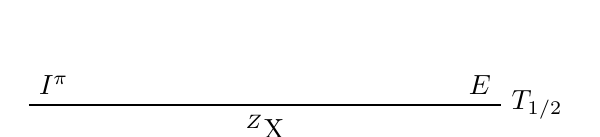
\begin{tikzpicture}
	\draw[thick](0, 0)node[above right]{$I^\pi$}--(6, 0)node[midway, below]{$\nucli ZX$}node[above left]{$E$}node[right]{$T_{1/2}$};
\end{tikzpicture}
\tikzchap 能态的描述
\end{center}
\paragraph{壳层模型}\index{壳层模型}原子的幻数:电子数为$2,10,18,36,54,86$时,元素特别稳定,意味着某些特定壳层的闭合。

核的幻数:质子数或中子数为$2,8,20,28,50,82,126$时,原子核特别稳定,是否也意味着壳层的闭合?

类比原子壳层模型,原子核的壳层结构模型假设:
\begin{compactenum}
	\item 每个能级上容纳的核子数目有一定的限制;
	\item 核子在核内的运动是独立的;

	Pauli原理既限制了每一能级所容纳核子的数目,同时也限制了原子核中核子间的碰撞概率——低能级的核子因碰撞而跃迁到较高能级的概率很小,这使得核子在核内有较大的自由程,单个核子可以在核内“独立运动”。
	\item 核内存在一平均场。

	虽无原子中不变的中心力场,但核子可以看成是在其它核子所形成的平均场中运动;对接近球形的原子核,可以认为这个力场是中心力场。
\end{compactenum}
谐振子势阱各能级的核子数为$2,6,12,20,\ldots$只能给出前三个幻数$2,8,20$,其他许多势阱模型也无法给出更好的结果。

1949年,M. G. Mayer和J. H. D. Jensen在势阱中加入了自旋-轨道耦合项,得到了幻数的关键项。(\nobel{1963})\index{自旋-轨道耦合}

总角动量量子数$j=\ell\pm 1/2$,每个能级上最多放$2j+1$个核子。
\begin{center}
	\tablechap{用字母表示轨道角动量}
	\begin{tabular}{cccccccc}
		\toprule
		&s&p&d&f&g&h&$\cdots$\\
		\midrule
		$\ell$&0&1&2&3&4&5&$\cdots$\\
		\bottomrule
	\end{tabular}
\end{center}
由于自旋-轨道耦合,原先1p能级会分裂成1p$_{1/2}$和1p$_{3/2}$两个能级,他们分别能容纳2和4个核子。自旋轨道平行的能级(即$\ell+1/2$)会比反平行(即$\ell-1/2$)能量更低,二者的能量差$\propto 2\ell+1$。
\begin{center}
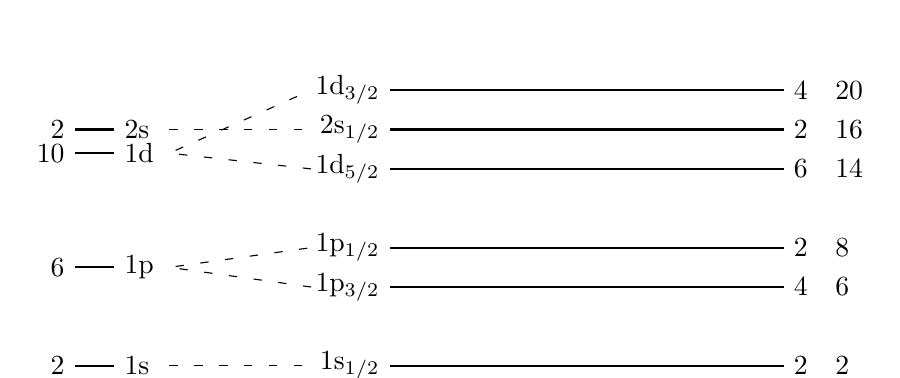
\begin{tikzpicture}
	% 1s
	\draw[thick](-4, 0)node[left]{2}--(-3.5, 0)node[right]{1s};
	\draw[loosely dashed](-2.8, 0)--(-1, 0);
	\draw[thick](0, 0)node[left]{1s$_{1/2}$}--(5, 0)node[right]{2\quad 2};
	% 1p
	\draw[thick](-4, 1.25)node[left]{6}--(-3.5, 1.25)node[right]{1p};
	\draw[loosely dashed](-1, 1)--(-2.8, 1.25)--(-1, 1.5);
	\draw[thick](0, 1)node[left]{1p$_{3/2}$}--(5, 1)node[right]{4\quad 6};
	\draw[thick](0, 1.5)node[left]{1p$_{1/2}$}--(5, 1.5)node[right]{2\quad 8};
	% 1d
	\draw[thick](-4, 2.7)node[left]{10}--(-3.5, 2.7)node[right]{1d};
	\draw[loosely dashed](-1, 2.5)--(-2.8, 2.7)--(-1, 3.5);
	\draw[thick](0, 2.5)node[left]{1d$_{5/2}$}--(5, 2.5)node[right]{6\quad 14};
	\draw[thick](0, 3.5)node[left]{1d$_{3/2}$}--(5, 3.5)node[right]{4\quad 20};
	% 2s
	\draw[thick](-4, 3)node[left]{2}--(-3.5, 3)node[right]{2s};
	\draw[loosely dashed](-2.8, 3)--(-1, 3);
	\draw[thick](0, 3)node[left]{2s$_{1/2}$}--(5, 3)node[right]{2\quad 16};
\end{tikzpicture}
\tikzchap 自旋-轨道耦合项引起的能级分裂示意图
\end{center}
\paragraph{基态核特点}
\begin{compactitem}
	\item 偶偶核中,成对成对核子间角动量方向相反,因此基态偶偶核自旋为0,宇称为$+$;
	\item 奇$A$核中其余偶数个核子的贡献相当于一个偶偶核的贡献,因此模型也叫\textit{单粒子模型}。最后一个奇核子的角动量$j$和轨道量子数$\ell$决定了自旋$j$,宇称$(-)^\ell$;
	\item 奇奇核自旋、宇称由两个奇核子状态决定。
\end{compactitem}
\clearpage
\section{原子核的放射性}
1895年Röntgen发现X射线(\nobel{1901});1896年Becquerel发现了铀的放射性质(\nobel{1903});1898年Rutherford从Becquerel射线中分离出了$\alpha$和$\beta$粒子(\nobel{1908}\footnote{这居然是个化学奖。});1900年Villard发现$\gamma$射线。
\begin{definition}{放射性术语}{radiation terminology}
	放射性:原子核自发地发射各种射线的现象。

	%放射性核素:能自发地发射各种射线的核素,也称为不稳定核素。

	衰变:原子核自发地发生转变的现象。
\end{definition}
原子核衰变的主要方式有$\alpha,\beta,\gamma$衰变、自发裂变、核子发射。

\paragraph{衰变纲图}\index{衰变纲图}
\begin{center}
	\begin{tikzpicture}
		\draw[ultra thick](-4, 5)node[above right]{\small$7/2^+$}--(0, 5)node[midway, below]{$\nucli{137}{Cs}$}node[above left]{\small 0}node[right]{\small\SI{30}{yr}};
		\draw[thick, latex-latex](1, 2)--(0, 5)--(1, 0);%node[midway, right]{94.4\%}node[midway, left]{5.6\%};
		\draw(.5, 3.5)--(-.5, 3)--(-3.5, 3)node[above right]{\small$\beta^-$ 511.6 94.6\%};
		\draw(.5, 2.5)--(-.5, 2)--(-3.5, 2)node[above right]{\small$\beta^-$ 1173.2 5.4\%};
		\draw[thick](1, 2)node[above right]{\small$11/2^-$}--(5, 2)node[above left]{\small 661.66}node[right]{\small$\SI{2.5}{min}$};
		\draw[ultra thick](1, 0)node[above right]{\small$3/2^+$}--(5, 0)node[midway, below]{$\nucli{137}{Ba}$(稳定)}node[above left]{\small 0}node[right]{\small stable};
		\draw[thick, latex-](3, 0)--(3, 2)node[right, rotate=60]{\small 661.66\enspace$\gamma$ 85.0\% e 9.6\%};%node[midway, right]{\small 661.66};
		\node[left]{$Q_{\beta^-}=\SI{1173.2+-0.9}{keV}$};
	\end{tikzpicture}
	\tikzchap 衰变纲图
\end{center}
\begin{compactenum}
	\item 主核素$\nucli{137}{Cs}$,基态自旋$7/2$,宇称$+$,能量$0$,半衰期$\SI{30}{yr}$;
	\item 子核素$\nucli{137}{Ba}$,基态自旋$3/2$,宇称$+$;激发态自旋$11/2$,宇称$-$,能量$\SI{661.66}{keV}$,半衰期$\SI{2.5}{min}$;
	\item 反映的是$\beta^-$衰变,然后子核由激发态$\gamma$跃迁到基态的物理过程;
	\item 能量变化:$\SI{1175.63}{keV},\SI{513.97}{keV},\SI{661.66}{keV}$;
	\item 绝对强度(概率):基态-基态5.4\%,基态-激发态94.6\%,$\gamma$射线85.0\%,内转换电子9.6\%。
	% \item $\gamma$跃迁
\end{compactenum} 
\subsection{放射性衰变的基本规律}
放射性原子核是全同的,原子核的衰变是独立、随机的。因此不能预测某一原子核的衰变时刻,放射性衰变是一个统计过程。

单一放射性具有指数衰减规律
\begin{align}
	\dv{N(t)}t=-\lambda N(t)\thus N(t)=N(0)\e{-\lambda t}.
\end{align}
其中$\lambda$为衰变常数\index{衰变常数},表示一个原子核在单位时间内发生衰变的概率。

定义衰变率$J(t)$为$t$时刻单位时间内衰变的核数目\index{衰变率}
\[
	J(t):=-\dv{N(t)}t\equiv\lambda N(t)
\]
\begin{definition}{分支比}{ratio}
	当一个原子核有几种衰变方式时,$\lambda$等于分支$\lambda_i$之和。
	%$\lambda=\sum_i\lambda_i$
	定义分支比\index{分支比}
	\begin{align}
		R_i:=\frac{\lambda_i}\lambda,
	\end{align}
\end{definition}
在衰变纲图中,并不是全部的绝对强度均为分支比,绝对强度的和也不一定为1,但主核素衰变的强度就是分支比。
\begin{definition}{半衰期、平均寿命、衰变宽度}{}
	半衰期$T_{1/2}$:\index{半衰期}原子核衰变为50\%所需要的时间
	\begin{align}
		\e{-\lambda T_{1/2}}=\frac12\thus T_{1/2}:=\frac{\ln 2}\lambda\doteq\frac{0.693}\lambda.
	\end{align}
	平均寿命$\tau$\index{平均寿命}
	\begin{align}
		\tau:=\int\zti t\cdot\lambda\e{-\lambda t}\d t=\frac1\lambda.
	\end{align}
	衰变宽度$\varGamma$,\index{衰变宽度}由波函数的FWHM (过程略)得
	\begin{align}
		\varGamma:=\hbar/\tau=\hbar\lambda.
	\end{align}
\end{definition}
\begin{definition}{放射性活度}{activity}
	放射性活度(activity)定义为单位时间内发生衰变的原子核数\index{活度}\footnote{明明就和衰变率完全一样(流汗黄豆)}
	\begin{align}
		A(t):=-\dv{N(t)}t\equiv\lambda N(t),
	\end{align}
	其SI单位为Becquerel,$\SI{1}{Bq}=\SI{1}{\per s}$。
\end{definition}
历史上也采用过Curie作为单位(\SI{1}{g} $\nucli{226}{Ra}$的活度)二者的关系是
\begin{align}
	\SI{1}{Ci}=\SI{3.7e10}{Bq}.
\end{align}

% 活度大小与原子核数目$N(t)$以及衰变常数$\lambda$有关。废话

比活度\index{比活度}定义为单位质量放射源的放射性活度。

\subsection{递次衰变规律}
\paragraph{两次连续衰变规律}
考虑一个两次连续衰变
\[
	\nuc A\overset{\lambda_1}{\longrightarrow }\nuc B\overset{\lambda_2}{\longrightarrow }\nuc C~(\mathrm{stable})
\]
核素A是单一放射性衰变,服从简单的指数规律
\[
	N_1(t)=N_{10}\e{-\lambda_1t}
\]
B的变化包括两方面:
\[
	\dv{N_2(t)}t=\lambda_1N_1(t)-\lambda_2N_2(t),
\]
故
\[\label{N2}
	N_2(t)=N_{10}\frac{\lambda_1}{\lambda_2-\lambda_1}(\e{-\lambda_1t}-\e{-\lambda_2t}).\tag{$\ast$}
\]
C仅由B衰变得到:
\[
	\dv{N_3(t)}t=\lambda_2N_2(t),
\]
故
\[
	N_3(t)=N_{10}\frac{\lambda_1\lambda_2}{\lambda_2-\lambda_1}\fkh{\frac1{\lambda_1}(1-\e{-\lambda_1t})-\frac1{\lambda_2}(1-\e{-\lambda_2t})}.
\]
显然$N_1(t)+N_2(t)+N_3(t)=N_{10}$。
\paragraph{多次连续衰变规律}
对于$n$代连续放射性衰变过程:
\[
	\nuc A_1\overset{\lambda_1}{\longrightarrow }\nuc A_2\overset{\lambda_2}{\longrightarrow }\cdots\overset{\lambda_n}{\longrightarrow }\nuc A_{n+1}(\mathrm{stable})
\]
一般的,有
\[
	N_n(t)=N_{10}\sum_{i=1}^nc_i\e{-\lambda_it},\quad c_i=\dvd{\prod_{k=1}^{n-1}\lambda_k}{\prod_{k\neq i}(\lambda_k-\lambda_i)}.
\]
\paragraph{放射性平衡}考虑两次连续衰变,经过一定时间衰变可能会形成平衡。
\subparagraph{暂时平衡}$T_1>T_2$但$T_1$不很大,会形成暂时平衡。\index{暂时平衡}平衡特点:
\begin{compactenum}
	\item 子体与母核数目将建立起固定的比例关系;
	\item 子体按照母核的半衰期衰减。
\end{compactenum}
由式(\ref{N2}),$N_2$和$A_2$存在极大值
\begin{align}
	\dv{N_2}t=0\thus t_\mathrm m=\frac{\ln\lambda_2-\ln\lambda_1}{\lambda_2-\lambda_1}.
\end{align}
$t_\mathrm m$时刻,$N_2$和$A_2$极大,且$A_1=A_2$。

$t>t_\mathrm m$时,$A_1<A_2$;$t\gg t_\mathrm m$时,子母核比例固定
%N_2(t)=\frac{\lambda_1}{\lambda_2-\lambda_1}N_1(t)(1-\e{-(\lambda_2-\lambda_1)t}).
\[
	\frac{N_2}{N_1}\doteq\frac{\lambda_1}{\lambda_2-\lambda_1},\quad\frac{A_2}{A_1}\doteq\frac{\lambda_2}{\lambda_2-\lambda_1}>1.
\]
\subparagraph{长期平衡}$T_1\gg T_2$且$T_1$很大。\index{长期平衡}虽然形式与暂时平衡相同,也有同样形式的$t_\mathrm m$,但$t\gg t_\mathrm m$后子母核活度相同:
\begin{align}
	\frac{A_2}{A_1}\doteq\frac{\lambda_2}{\lambda_2-\lambda_1}\doteq 1.
\end{align}
子核也是按着母核的半衰期衰变。

\subparagraph{不成平衡}$T_1<T_2$,时间足够长之后,母核就衰变完了,只有子核按自己的半衰期衰变。\index{不成平衡}

以上三种平衡均存在子母核活度关系的转折点$t_\mathrm m$,且受更短半衰期的核的影响更大。
\subsection{放射系}
地球上目前存在三个天然放射系:\index{放射系}
\begin{align*}
	\text{钍系}&&^{232}_{~90}\mathrm{Th},&\quad T_{1/2}=\SI{1.4e10}{yr},\\
	\text{铀系}&&^{238}_{~92}\mathrm{U},&\quad T_{1/2}=\SI{4.468e9}{yr},\\
	\text{锕铀系}&&^{235}_{~92}\mathrm{U},&\quad T_{1/2}=\SI{7.038e8}{yr}.
\end{align*}
这些都形成了长期平衡,子核的活度与母核相同。

放射系以$_{82}$Pb为终点,导致其母核$_{84}$Po半衰期一般都很短。
\subsection{放射规律的一些应用}
\paragraph{放射源活度修正}
\[
	A(t)=A(0)\e{-\lambda t}=\lambda N(0)\e{-\lambda t}.
\]
\paragraph{确定放射源性质}略,见讲义
\paragraph{确定放射源活度和制备时间}人工制备放射源时,如何确定源的活度和最佳制备时间?例
\[
	\nton+\nuc A\to\nuc B+\gamma,
\]
若粒子束的强度是一定的,则放射性核素B的产生率
\begin{align}
	P=N_{\mathrm{target}}\sigma_0\Phi,
\end{align}
是恒定不变的,式中$N_{\mathrm{target}}$是靶核A的数量,$\sigma_0$表示$\nton$与A的反应截面($\si{cm^2}$),$\Phi$表示中子注量率($\si{1/cm^2\cdot s}$)。

而生产的放射性核素又在不断地衰变,故
\[
	\dv{N(t)}t=P-\lambda N(t),
\]
故源的活度应为
\begin{align}
	A(t)=P(1-\e{-\lambda t}).
\end{align}
与$N_{\mathrm{target}},\sigma_0,\Phi,\lambda,t$五个因素有关。
定义饱和因子$S:=1-\e{-\lambda t}$。\index{饱和因子}
\paragraph{放射性鉴年法}$\nucli{14}C$具有$\beta^-$放射性
\[
	\nucli{14}C\to\nucli{14}N+\elc^-+\bar\nu_\elc,
\]
半衰期5700年。

而宇宙射线一直与大气层中的核发生反应,产生中子
\[
	\nton+\nucli{14}N\to\nucli{14}C+\pton.
\]
大气与生物体中$\nucli{12}C$与$\nucli{14}C$比例是一定的。生物死后体内$\nucli{14}C$不断衰变。
\paragraph{短寿命核素发生器}
核医学需要短寿命放射性核素作为标记核素,可以利用“母牛”生产这些核素并运输到医院等需要使用的地方。比如
\[
	\nucli{99}{Mo}\enspace\mathop{\semilongrightarrow}\limits^{\beta^-}_{\SI{66}{h}}\enspace\nucli{99m}{Tc}\enspace\mathop{\semilongrightarrow}\limits^{\mathrm{IT}}_{\SI{6}{h}}\enspace\nucli{99}{Tc},
\]
$t_\mathrm m=\SI{20.8}{h}$时,子核放射性活度最大,淋洗交换柱。
\clearpage
\section{原子核的衰变}
不稳定核在嬗变成(更)稳定原子核的过程中,会发生$\alpha$衰变、$\beta$衰变、$\gamma$跃迁、中子发射、质子发射或自发裂变等过程。

\subsection[\textit{\textalpha}衰变]{$\alpha$衰变}
$\alpha$衰变的形式:
\begin{align}
	{^A_Z\nuc X} \to {^{A-4}_{Z-2}\nuc Y} + {^4_2\nuc{He}}.
\end{align}
%子核较母核减少了2个质子和2个中子。
%由于$\beta$稳定曲线偏向$N$轴,位于$\beta$稳定曲线上的母核发生$\alpha$衰变后,子核会偏离$\beta$稳定曲线,故子核可能会接着发生$\beta$衰变。
$\alpha$衰变的特点:
\begin{compactenum}
	\item 重核$A>140$;
	\item 能量既不太大也不太小$\SIrange{4}{9}{MeV}$;
	\item 半衰期范围较大$\SI{e-7}{s}\vs\SI{e15}{yr}$。
\end{compactenum}
由液滴模型,$\alpha$衰变主要项是Coulomb排斥。

自发的衰变需要释放能量,由比结合能曲线:不存在发射$\nucli2H$核的衰变,重核发生$\alpha$衰变将释放能量,子核也比母核更稳定。\footnote{事实上释放$\nucli{12}C$等粒子的衰变释放能量更多,子核更稳定,但是其发生概率太小。}

\subsubsection[\textit{\textalpha}衰变能]{$\alpha$衰变能}
对于静止\footnote{母核热运动的动能$\ll\alpha$衰变的衰变能。}的母核,衰变前后有能量守恒
\[
	m_{\nuc X}c^2=m_{\nuc Y}c^2+m_\alpha c^2+T_{\nuc Y}+T_\alpha
\]
$\alpha$衰变能就等于子核$\nuc Y$和$\alpha$粒子的动能之和,即衰变前后静止质量之差
\begin{align}
	E_0&=T_{\nuc Y}+T_\alpha=\bigfkh{m_{\nuc X}-(m_{\nuc Y}+m_\alpha)}c^2\\\notag
	&=\D(\nuc X)-\D(\nuc Y)-\D(\alpha)
\end{align}
故$\alpha$衰变的必要条件为$E_0>0$
\[
	M(\nuc X)>M(\nuc Y)+M(\alpha)
\]

由液滴模型的Coulomb能:$A,Z$越大,$\alpha$衰变能越大;但是对于同位素$A$越大,$\alpha$衰变能越小。

壳层结构给出:母核$N=126$时,$\alpha$衰变能很小;子核$N=126$时,$\alpha$衰变能局部极大。

\paragraph{$\alpha$衰变能与核能级图}
由静止母核发生$\alpha$衰变前后的能量、动量守恒推出
\begin{align}
	E_0=\frac{A}{A-4}T_\alpha
\end{align}
故可以通过测量$\alpha$粒子的能量$T_\alpha$得到$\alpha$衰变能$E_0$。\footnote{Y的轨迹$\ll\alpha$粒子,难以测量其能量。}

然而,单一能级衰变的母核可能衰变出不同能级的子核,导致$\alpha$粒子有多个能量。衰变能之间的差对应子核的能级结构。
其中,最大衰变能很有可能就是子核的基态。
\iffalse
基态-基态的$\alpha$衰变能为
\begin{align}
	E_0=M(\nuc X)-M(\nuc Y)-M(\alpha),
\end{align}
式中皆为基态质量。
\fi
\begin{center}
	\begin{tikzpicture}
		\node[right]at(4, -.5){$Q_\alpha=\SI{5407.63+-0.10}{keV}$};
		\draw[ultra thick](0, 0)node[above right]{\small $0^+$}--(4, 0)node[midway, below]{$\nucli{206}{Pb}$ (稳定)}node[above left]{\small 0};
		\draw[thick](0, 2)node[above right]{\small $2^+$}--(4, 2)node[above left]{\small 803.1};
		\draw[thick, latex-](2, 0)--(2, 2)node[right, rotate=60]{\small 804\enspace$\gamma$ \num{0.00107}\%};
		\draw[thick, latex-](4, 2)--(5, 2)node[right]{\small\enspace\num{4524}\qquad\num{0.00107}};
		\node[above right]at(5, 2.1){\small$E_\alpha(\si{eV})\qquad I_\alpha(\%)$};
		\draw[thick](5, 0)--(5, 6);
		\draw[thick, latex-](4, 0)--(5.05, 0)node[right]{\small\num{5304.61}\qquad 99}--(5.05, 5.95);
		\draw[thick](4.95, 6.05)--(5.1, 5.9);
		\draw[thick](4.95, 6.15)--(5.1, 6);
		\draw[thick](5, 6.1)--(5, 7);
		\draw[thick](5.05, 6.05)--(5.05, 7);
		\draw[ultra thick](5, 7)node[above right]{\small $0^+$}--(9, 7)node[midway, below]{$\nucli{210}{Po}$}node[right]{\small\SI{138.38}{d}};
	\end{tikzpicture}
	\tikzchap $\alpha$衰变的衰变纲图
\end{center}
\subsubsection[\textit{\textalpha}衰变的衰变常数]{$\alpha$衰变的衰变常数}
$\alpha$粒子在核内主要受核力和Coulomb力。其中核内所受合力平衡,所以$\alpha$粒子在核内自由地高速运动。

隧穿理论:$\alpha$粒子相对于子核的势能
\begin{align}
	V(r)=\begin{cases}
		-V_0,&r<R\\
		\frac1{4\pi\varepsilon_0}\frac{2Z_{\nuc Y}e^2}r,&r\geqslant R
	\end{cases}
\end{align}
其中$R=R_\alpha+R_{\nuc Y}$。
\begin{center}
	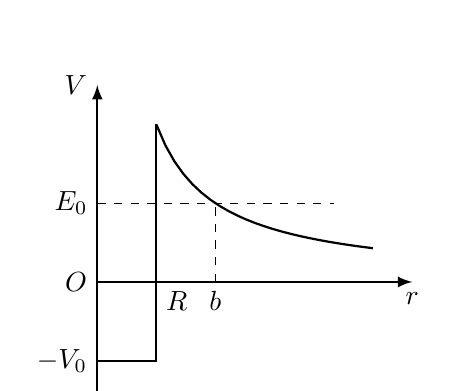
\begin{tikzpicture}
		\draw[thick, -latex](0, -1.5)--(0, 2.5)node[left]{$V$};
		\draw[thick, -latex](0, 0)node[left]{$O$}--(4, 0)node[below]{$r$};
		\draw[dashed](0, 1)node[left]{$E_0$}--(3, 1);
		\draw[thick](0, -1)node[left]{$-V_0$}--(.75, -1)--(.75, 2);
		\draw[dashed](1.5, 0)node[below]{$b$}--(1.5, 1);
		\node[below right]at(.75, 0){$R$};
		\draw[thick, domain=.75:3.5]plot(\x, {1.5/\x});
	\end{tikzpicture}
	\tikzchap Coulomb势垒
\end{center}
量子力学中我们学过,能量为$E$质量为$m$的粒子穿过高度为$V_0$宽度为$a$的方势垒的概率为
\[
	P=\exp\fkh{-\frac{2a}\hbar\sqrt{2m(V_0-E)}},
\]
若衰变发生,$\alpha$粒子需要穿过Coulomb势垒
\[
	P=\exp\fkh{-2\frac{\sqrt{2\mu}}\hbar\int_R^b\sqrt{V(r)-E_0}\d r}=:\e{-G},
\]
式中$\mu=\frac{m_\alpha m_{\nuc Y}}{m_\alpha+m_{\nuc Y}},b=\frac{2Z_\nuc Ye^2}{4\pi\varepsilon_0 E_0}$其中$G$为Gamow因子。对于$b\gg R$有
\[
	P=\e{-G}=\exp\fkh{-\frac{e^2\sqrt{2m_\alpha}}{2\varepsilon_0\hbar}\cdot\frac{Z_\nuc Y}{\sqrt{E_0}}+\frac{4e\sqrt{m_\alpha }}{\sqrt{\pi\varepsilon_0\hbar}}\sqrt{RZ_\nuc Y}}
\]
这个概率乘上$\alpha$粒子到达边界的频率
\[
	n=\frac{\nu}{2R}\doteq\frac1{2R}\sqrt{\frac{2(E_0+V_0)}{m_\alpha}}\doteq\SI{2.44e21}{/s}.
\]
就得到了衰变常数$\lambda=nP$。
\begin{align}
	\lg\lambda=C-1.72\times Z_{\nuc Y}E_0^{-1/2}
\end{align}
式中$C$是影响较小的其他项。

对于奇$A$核和奇奇核,理论与实验差别较大:引入阻碍因子(Hindrance factor):
\begin{compactenum}
	\item 形成因子:$\alpha$粒子并非早已存在,是在衰变过中产生的;
	\item 角动量:会产生离心势$\frac{\ell(\ell+1)\hbar^2}{2m_\alpha R^2}.$
\end{compactenum}
\paragraph{总结}
\begin{compactenum}
	\item $\alpha$粒子穿透势垒的概率$P$是决定衰变常数$\lambda$的最主要因素;衰变能$E_0$越大,所需要穿透的势垒越薄,$\lambda$越大,衰变得越快。
	\item $\alpha$粒子还可能带走角动量,离心势会加高势垒,减小了衰变常数。
\end{compactenum}
让衰变能大一些,让$\alpha$粒子带的角动量小一点,有利于$\alpha$衰变的发生。
\subsubsection[{\textit{\textalpha}衰变的宇称和角动量}]{$\alpha$衰变的宇称和角动量}
$\alpha$衰变过程中角动量守恒,若母子核的角动量分别为$I_\ini,I_\fin$,则$\alpha$粒子的角动量$\ell_\alpha$可取
\begin{align}
	\ell_\alpha=|I_\ini-I_\fin|,\ldots,I_\ini+I_\fin
\end{align}
共$2\min\{I_\ini,I_\fin\}+1$种情况。

在强相互作用和电磁相互作用中,宇称是守恒的。$\alpha$粒子的宇称$(-)^{\ell_\alpha}$,因此初末态宇称若不满足
\begin{align}
	\pi_\ini=\pi_\fin\cdot(-)^{\ell_\alpha},
\end{align}
则$\alpha$衰变不可能发生!
\subsection[\textit{\textbeta}衰变]{$\beta$衰变}
原子核自发地放出$\beta$粒子或俘获轨道电子,并转变成另一种原子核的现
象,称为$\beta$衰变,有三种形式:
\begin{compactenum}
	\item $\beta^-$衰变:原子核衰变时发射负电子;
	\item $\beta^+$衰变:原子核衰变时发射正电子;
	\item 轨道电子俘获(orbital electron capture, EC,也称$\varepsilon$衰变):原子核从核外的电子壳层俘获一个轨
	道电子。
\end{compactenum}

由于质子中子之间质量存在差异
\[
	m_\nton - m_\pton = \SI{1.293}{\MeV}/c^2 > m_\elc = \SI{0.511}{MeV}/c^2
\]
故自由中子可以发生$\beta^-$衰变:
\[
	\nton\to\pton+\elc^-\textcolor{lightgray}{\,+\,\bar\nu_\elc},
\]
而自由质子(即$\nucli1H$)不能发生$\beta^+$衰变和EC:
\begin{gather*}
	\pton\nrightarrow \nton+\elc^+\textcolor{lightgray}{\,+\,\nu_\elc},\\
	\pton+\elc^-\nrightarrow \nton\textcolor{lightgray}{\,+\,\nu_\elc},
\end{gather*}
只有结合在核中的质子才行。

\paragraph{$\beta$衰变的特点}
\begin{compactenum}
	\item $\beta$衰变核素遍及整个元素周期表;
	\item $\beta$衰变不改变$A$,子母核同属等量异位素;
	\item $\beta$衰变电子能谱分布是连续的:$\si{keV}\vs\si{MeV};$
	\item 半衰期范围$10^{-3}\,\mathrm{s}\vs\SI{e24}{yr}.$
\end{compactenum}
由于$\beta$衰变不改变$A$,考虑液滴模型(\ref{liquid-drop model BE})中与$Z$有关的项
\[
	B=\textcolor{lightgray}{a_VA-a_SA^{2/3}}-a_\mathrm C\frac{Z^2}{A^{1/3}}-a_\mathrm{sym}\frac{(A/2-Z)^2}{A}+a_\mathrm p\frac{\delta}{A^{1/2}},
\]
得出质量
\[
	M(Z,A)=\textcolor{lightgray}{Am_\nton\,+\,}Z\bigkh{M(\nucli1H)-m_\nton}+B,
\]
Coulomb能、对称能使得等量异位素的结合能是一条抛物线,%而最稳定的核素约处于$Z=A/2$的位置,
小$Z$会发生$\beta^-$衰变,大$Z$会发生$\beta^+$衰变或EC;对于偶$A$核,由于对能项,奇奇核与偶偶核会有各自的抛物线。

\paragraph{$\beta$-ray's wrong energy}子核能级分立,但$\beta$粒子的能量是连续的?
\begin{compactitem}
	\item 假说1:子核能级密集$\nleftarrow$~$\gamma$能谱不连续;
	\item 假说2:$\beta$粒子与介质作用损失了不等的能量$\nleftarrow$厚壁量热器实验。
\end{compactitem}
Pauli中微子假说(1930):原子核在$\beta$衰变的过程中,不仅放出一个$\beta$粒子,同时还放出一个中性微小粒子。
\paragraph{中微子假说}中微子性质:
\begin{compactenum}
	\item 电荷为0;
	\item 自旋为$\hbar/2$,是Fermi子;
	\item 质量非常小,\href{https://www.sciencedirect.com/topics/chemistry/electron-neutrino}{$<\SI{0.07}{eV}/c^2$},\footnote{中微子震荡(\nobel{2015})表明中微子质量不严格是0。}与电子相比,可以看作0;
	\item 磁矩非常小,\href{https://arxiv.org/ftp/arxiv/papers/1506/1506.01284.pdf}{$\sim 10^{-19}\muB$};
	\item 与物质的相互作用非常弱,属弱相互作用。
\end{compactenum}
$\nu$和$\bar\nu$互为反粒子,$\nu$左旋,$\bar\nu$右旋。相互作用性质不同。
\subsubsection[\textit{\textbeta}衰变的三种类型]{$\beta$衰变的三种类型}
$\beta^-,\beta^+,$EC:
\begin{align}
	\beta^-:&\qquad{^A_Z\nuc X} \to {^{\quad\!A}_{Z+1}\nuc Y} + \elc^- + \bar\nu_\elc,\\
	\beta^+:&\qquad{^A_Z\nuc X} \to {^{\quad\!A}_{Z-1}\nuc Y} + \elc^+ + \nu_\elc,\\
	\mathrm{EC}:&\qquad{^A_Z\nuc X} + \elc^- \to {^{\quad\!A}_{Z-1}\nuc Y} + \nu_\elc
\end{align}
丰中子核素大多具有$\beta^-$衰变,比如天然放射系、重核裂变、$(n,\gamma)$反应后的核素;丰质子核素可以发生$\beta^+$衰变或EC,比如$(\gamma,n)$反应后的核素。

定义:$\beta^-$衰变放出的动能$T_{\nuc Y}+T_{\beta^-}+T_{\bar\nu_\elc}$为$\beta^-$衰变能。
\begin{align}\notag
	E_0(\beta^-)&=[m(\nuc X)-m(\nuc Y)-m_\elc]c^2\\\notag
	&\doteq[M(\nuc X)-\cancel{Zm_\elc}-M(\nuc Y)+\cancel{(Z+1)m_\elc}-\cancel{m_\elc}]c^2\\
	&=[M(\nuc X)-M(\nuc Y)]c^2\\\notag
	&=\D(Z,A)-\D(Z+1,A);
\end{align}
$\beta^+$和EC衰变能定义类似:
\begin{align}
	E_0(\beta^+)&=[M(\nuc X)-M(\nuc Y)-2m_\elc]c^2;\\
	E_0(\varepsilon)&=[M(\nuc X)-M(\nuc Y)]c^2-\varepsilon_i.
\end{align}
其中,$\varepsilon_i(i=\mathrm{K,L,M,}\ldots)$为被俘获电子与母核的结合能,
\begin{align*}
	\varepsilon_{\mathrm K}&\doteq(Z-1)^2\,\si{Ry},\\
	\varepsilon_{\mathrm L}&\doteq\frac14(Z-5)^2\,\si{Ry},\\\
	\varepsilon_{\mathrm M}&\doteq\frac19(Z-13)^2\,\si{Ry}.
\end{align*}
其中$\si{Ry}$是Rydberg能量单位,$\SI{1}{Ry}=\SI{13.6}{eV}$。

一般都是K层电子最容易发生俘获,但当衰变能不高时,就会发生L层俘获,满足
\[
	\varepsilon_\mathrm K / c^2 > M(\nuc X)-M(\nuc Y) > \varepsilon_\mathrm L / c^2
\]

当EC发生时,原子会发射特征X射线以及Auger电子。比如当K层电子被俘获时,子核的L层电子就会向K层跃迁,产生能量为$\varepsilon_\mathrm K - \varepsilon_\mathrm L$的X射线;该能量也可以直接给予L层的电子使其电离,产生能量为$\varepsilon_\mathrm K - 2\varepsilon_{\mathrm L}$的Auger电子。

由于衰变能限制,因此发生$\beta$衰变的能量条件为:
\begin{align}
	\beta^-:&\qquad M(\nuc X)>M(\nuc Y)\\
	\beta^+:&\qquad M(\nuc X)-M(\nuc Y) > 2m_\elc,\\
	\mathrm{EC}:&\qquad M(\nuc X)-M(\nuc Y) > \varepsilon_i / c^2.
\end{align}
由于
\[
	2m_\elc c^2=\SI{1.022}{MeV}\gg\varepsilon_i,
\]
故若可以发生$\beta^+$衰变,则一定也可以发生EC。对于衰变能较大的轻核,$\beta^+$衰变概率显著,重核反之,中等质量核二者几率相仿。一些核(如$\nucli{64}{Cu}$)可能同时满足三个条件,可以同时以三种方式进行衰变。
\begin{center}
	\begin{tikzpicture}
		\draw[ultra thick](0, 4)node[above right]{\small$1^+$}--(4, 4)node[midway, below]{$\nucli{64}{Cu}$}node[right]{\small\SI{12.70}{h}};
		\draw[ultra thick](-4, 0)node[above right]{\small$0^+$}--(-1, 0)node[midway, below]{$\nucli{64}{Ni}$(稳定)}node[above left]{\small0};
		\draw[thick](-4, 3)node[above right]{$2^+$}--(-1, 3)node[above left]{\small\num{1345.8}};
		\draw[ultra thick](5, 2.5)node[above right]{\small$0^+$}--(7, 2.5)node[midway, below]{$\nucli{64}{Zn}$(稳定)};
		\draw[thick, -latex](4, 4)--(5, 2.5);
		\draw[thick, -latex](0, 4)--(-1, 3);
		\draw[thick, -latex](0, 4)--(-1, 0);
		\draw[thick, -latex](0, 4)--(0, 2)--(-1, 0);
		\draw[thick, latex-](-2.8, 0)--(-2.8, 3)node[right, rotate=60]{\small\num{1345.77}\enspace$\gamma$ \num{0.48}\%};
		\draw(4.5, 3.25)--(4, 2.8)--(.5, 2.8)node[above right]{\small$\beta^-$\enspace\SI{578.2}{keV} 37.1\%}node[below right]{\small $Q_{\beta^-}=\SI{578.2+-1.5}{keV}$};
		\draw(-.5, 3.5)--(.5, 1.65)node[above right]{\small EC$_1$}--(4, 1.65)node[above left]{\small 0.48\%};
		\draw(-.5, 2)--(.5, 1)node[above right]{\small EC$_2$}--(4, 1)node[above left]{\small 44.5\%};
		\draw(-.5, 1)--(.5, .35)node[above right]{\small$\beta^+$\enspace\SI{652.9}{keV}\enspace\,17.9\%}node[below right]{\small$Q_{\mathrm{EC}}=\SI{1674.9+-0.8}{keV}$}--(4, .35);
	\end{tikzpicture}
	\tikzchap $\nucli{64}{Cu}$的衰变纲图
\end{center}
\subsubsection[\textit{\textbeta}衰变的Fermi理论和选择定则]{$\beta$衰变的Fermi理论和选择定则}
$\beta$粒子从何而来?
\begin{compactenum}
	\item 质子和中子是核子两种不同的量子态,$\beta$衰变是核中质子和中子两种量子态之间的跃迁;
	\item 核子两种量子态跃迁过程中放出电子和中微子,它们是核子不同状态跃迁的产物;
	\item $\beta$衰变中放出电子和中微子,电子-中微子场与原子核的相互作用为弱相互作用,半衰期($\SI{e-3}{s}\vs\SI{e18}{yr}$)比电磁相互作用($\SIrange{e-16}{e-4}{s}$)要长得多。
\end{compactenum}
Fermi黄金规则
\begin{align}
	\lambda = \frac{2\pi}\hbar\abs{V_{\fin\ini}}^2\rho(E_\fin),
\end{align}
式中$V_{\fin\ini}$是跃迁矩阵元,$\rho(E_\fin)$是末态密度。

量子力学的微扰理论给出:单位时间发射动量处于$(p,p+\d p)$间的$\beta$粒子的概率为:
\[
	I(p_\beta)\d p_\beta=\frac{2\pi}\hbar\abs{\int\psi_\fin\cj H\psi_\ini\d^3r}^2\dv n{T_\beta}
\]
初态$\psi_\ini=u_\ini$母核波函数,末态$\psi_\fin=u_\fin\varphi_\beta\varphi_\nu$子核、$\beta$和中微子波函数,$H=g$描述弱作用强度:
\[
	I(p_\beta)\d p_\beta=\frac{2\pi g^2}\hbar\abs{\int u_\fin\cj\varphi_\beta\cj\varphi_\nu\cj u_\ini\d^3r}^2\dv n{T_\beta}
\]

原子核对电子和中微子的波场影响很小,可视电子(近似)和中微子为自由粒子,波函数用平面波描述
\[
	\varphi_\beta\cj=V^{-1/2}\e{-\i\bm k_\beta\cdot\bm r},\quad\varphi_\nu\cj=V^{-1/2}\e{-\i\bm k_\nu\cdot\bm r}
\]
则上式化作
\[
	I(p_\beta)\d p_\beta=\frac{2\pi g^2}{\hbar V^2}\abs{M_{\ini\fin}}^2\dv n{T_\beta}
\]
其中跃迁矩阵元
\begin{align}\label{transition matrix element}
	M_{\ini\fin}=\int u_\fin\cj u_\ini\e{-\i(\bm k_\beta+\bm k_\nu)\cdot\bm r}\d^3r
\end{align}

\paragraph{末态密度}$\beta$和中微子状态数
\[
	\d n_\beta=\frac V{h^3}4\pi p_\beta^2\d p_\beta,\quad \d n_\nu=\frac V{h^3}4\pi p_\nu^2\d p_\nu
\]
故末态密度
\[
	\dv n{T_\beta}=\frac{p_\beta^2p_\nu^2\d p_\beta\nd p_\nu}{4\pi^4\hbar^6\d T_\beta}V^2
\]
忽略子核反冲动能\footnote{因为子核质量$\gg$轻子。},则:
\[
	T_\nu+T_\beta=E_0
\]
考虑到$m_\nu=0,T_\nu=cp_\nu$
\[
	p_\nu=\frac{E_0-T_\beta}c,\quad\dv{p_\nu}{T_\beta}=-\frac1c.
\]
带入上式
\[
	\dv n{T_\beta}=\frac{p_\beta^2(E_0-T_\beta)^2\d p_\beta}{4\pi^4\hbar^6c^3}V^2
\]
故$m_\nu=0$时的$\beta$跃迁几率公式
\begin{align}\label{beta-decay Prob}
	I(p_\beta)\d p_\beta=\frac{g^2\abs{M_{\ini\fin}}^2}{2\pi^3\hbar^7c^3}\kh{E_0-\sqrt{p_\beta^2c^2+m_\elc^2c^4}+m_\elc c^2}^2p_\beta^2\d p_\beta
\end{align}
\begin{center}
	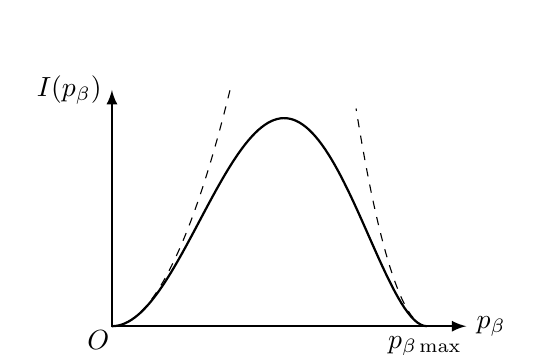
\begin{tikzpicture}
		\coor{4.5}{3}{p_\beta}{I(p_\beta)};
		\draw[thick, domain=0:4, samples=100]plot(\x, {(2-sqrt(\x^2+9)+3)^2*\x^2/3})node[below]{$p_{\beta\max{}}$};
		\draw[dashed](0, 0)parabola(1.5, 3);
		\draw[dashed](4, 0)parabola(3.1, 2.7648);
	\end{tikzpicture}
	\tikzchap 末态密度$I(p_\beta)$随$\beta$粒子动量$p_\beta$的关系
\end{center}
若$p_\beta$很小,则
\[
	I(p_\beta)\doteq\frac{g^2\abs{M_{\ini\fin}}^2}{2\pi^3\hbar^7c^3}E_0^2p_\beta^2\propto p_\beta^2;
\]
若$p_\beta$与最大值$p_{\beta\max{}}$相差$\D p_\beta$很小,则
\[
	I(p_\beta)\doteq\frac{g^2\abs{M_{\ini\fin}}^2}{2\pi^3\hbar^7c^3}\kh{\frac{p_{\beta\max{}}^2c^2}{E_0+m_\elc c^2}}^2\D p_\beta^2\propto\D p_\beta^2.
\]
因此$\beta$谱在两端会呈现两个抛物线。

末态密度项决定了$\beta$粒子的动量谱的形状,会影响衰变速度。

事实上,$\beta$粒子还受核Coulomb场的影响,式(\ref{beta-decay Prob})还应加上Coulomb修正因子(Fermi function)
\begin{align}\label{Fermi funtion}
	I(p_\beta)\d p_\beta=\frac{g^2\abs{M_{\ini\fin}}^2}{2\pi^3\hbar^7c^3}F(Z,T_\beta)(E_0-T_\beta)^2p_\beta^2\d p_\beta
\end{align}
当$Z$较小时,用非相对论近似
\[
	F(Z,T_\beta)=\frac x{1-\e{-x}},\qquad x=\pm\frac{2\pi\alpha Zc}{v_\beta},\quad\text{for}~\beta^\mp.
\]
\paragraph{跃迁矩阵元}在相同动能的情况下,由
\[
	\Ek+mc^2=\sqrt{p^2c^2+m^2c^4},\thus p=\frac1c\sqrt{\Ek^2+2\Ek mc^2},
\]
知,电子带走的动量/角动量更多。

对式(\ref{transition matrix element})跃迁矩阵元中的轻子项做Taylor展开
\begin{align*}
	\exp\fkh{-\frac\i\hbar(\bm p_\beta+\bm p_\nu)\cdot\bm r}=\sum_{\ell=0}^\infty\frac{(-\i)^\ell}{\ell!}\fkh{\frac{(\bm p_\beta+\bm p_\nu)\cdot\bm r}\hbar}^\ell.
\end{align*}
以衰变能$E_0=\SI{1}{MeV}$估计,当电子获得全部衰变能时,轻子组的动量最大,因此有
\[
	\abs{\frac{(\bm p_\beta+\bm p_\nu)\cdot\bm r}\hbar}\leqslant\frac{E_0r}{\hbar c}=\frac{\SI{1}{MeV}\cdot\SI{1.2}{fm}}{\SI{197.4}{MeV.fm}}A^{1/3}<0.05.
\]
故在级数中,第一项贡献最大,以后各项依次很快递减。

或将平面波按不同的轨道角动量$\ell$正交分解为球面波
\[
	\e{-\i(\bm k_\beta+\bm k_\nu)\cdot\bm r}=\sum_{\ell=0}^\infty(2\ell+1)(-\i)^\ell j_\ell\bigkh{(\bm k_\beta+\bm k_\nu)\cdot\bm r}P_\ell(\cos\theta)
\]
球Bessel函数在$kr\ll 1$下的近似为
\[
	j_\ell(kr)\doteq\frac{(kr)^\ell}{(2\ell+1)!}.
\]
Legendre多项式的内积
\[
	\int P_\ell(\cos\theta)P_{\ell'}(\cos\theta)\sin\theta\d\theta\nd\phi=\frac{4\pi}{2\ell+1}\vd_{\ell\ell'}.
\]
故$\ell=0,1,2,\ldots$各项出现的概率
\begin{center}
	\begin{tabular}{cccccc}
		\toprule
		$\ell$&0&1&2&3&$\cdots$\\
		\midrule
		&1&$\frac{(kr)^2}3$&$\frac{(kr)^4}{45}$&$\frac{(kr)^6}{1575}$&$\cdots$\\
		\bottomrule
	\end{tabular}
\end{center}
第1项贡献最大,以后各项依次很快递减,若$\ell=0$被允许有贡献,此时的跃迁被称为\textbf{允许跃迁},对应的矩阵元称为原子核矩阵元$M$,与轻子无关。

允许跃迁有大的衰变常数,但当其被禁戒而贡献为0时,就要考虑禁戒跃迁。$\ell=n\hbar$称为$n$级禁戒跃迁。每级相差$10^{-4}.$
\paragraph{选择定则}在$\beta$衰变的孤立系统中角动量守恒,母子核的角动量差由两个轻子的自旋和轨道角动量决定。
\[
	\bm I_\ini=\bm I_\fin+\bm\ell+\bm s.
\]

\subparagraph{允许跃迁}
$\ell=0$。电子和中微子自旋均为$1/2$,这时$s$只有0和1两种取值:
\begin{compactenum}
	\item 若$s=0$,电子和中微子自旋反平行,单态,
	\[
		\D I=I_\ini-I_\fin=0,
	\]
	称为Fermi选择定则,F跃迁,F相互作用;
	\item 若$s=1$,电子和中微子自旋平行,三重态,
	\[
		\D I=0,\pm 1,
	\]
	称为Gamow-Teller选择定则,G-T跃迁,G-T相互作用。
\end{compactenum}
允许跃迁的宇称选择定则
\[
	\D\pi=(-)^0=+.
\]
\subparagraph{一级禁戒跃迁}
$\ell=1$,则$\abs{\ell+s}=0,1,2$,故一级禁戒跃迁的自旋和宇称选择定则为
\[
	\D I=0,\pm 1,\pm 2,\quad\D\pi=-.
\]
\subparagraph{二级禁戒跃迁}
按理说,自旋选择定则$\D I=0,\pm 1,\pm 2,\pm 3$,但实际为$\D I=\pm 2,\pm 3$,因为低级的跃迁竞争更强。宇称选择定则$\D\pi=+.$
\begin{center}
	\tablechap{$\beta$衰变自旋和宇称的选择定则}
	\begin{tabular}{cccc}
		\toprule
		跃迁类型&$\ell$&$\D I$&$\D\pi$\\
		\midrule
		允许跃迁&0&$0,\pm 1$&$+$\\
		一级禁戒跃迁&1&$0,\pm 1,\pm 2$&$-$\\
		二级禁戒跃迁&2&$\pm 2,\pm 3$&$+$\\
		$\cdots$&$\cdots$&$\cdots$&$\cdots$\\
		$n$级禁戒跃迁&$n$&$\pm n,\pm(n+1)$&$(-)^n$\\
		\bottomrule
	\end{tabular}
\end{center}
\subsubsection[\textit{\textbeta}能谱形状与Kurie描绘]{$\beta$能谱形状与Kurie描绘}
为验证Fermi理论,将式(\ref{Fermi funtion})改写为
\[
	\fkh{\frac{I(p_\beta)}{F(Z,T_\beta)p_\beta^2}}^{1/2}=\frac{g\abs{M_{\ini\fin}}}{\sqrt{2\pi^3\hbar^7c^3}}(E_0-T_\beta)\propto(E_0-T_\beta).
\]
画在坐标图上是一条直线,这就是Kurie图\footnote{Kurie Plot,是Franz N. D. Kurie提出的,中文翻译为库里厄图或居里描绘,跟居里夫妇(Curie)没关系。}

允许跃迁的Kurie图中,由于源的自吸收和散射,在低能区会偏离直线,但高能区线性很好,且与横轴的交点就是衰变能$E_0.$

禁戒跃迁的$M_{\ini\fin}\neq M$与$p_\beta,p_\nu$有关,Kurie图不再是直线,需要加上形状因子(shape factor)修正为直线。
\paragraph{总结}决定$\beta$能谱形状由式(\ref{Fermi funtion})决定,共三个因子:
\begin{compactenum}
	\item 统计因子$(E_0-T_\beta)^2p_\beta^2\d p_\beta$,反映了末态密度数,电子动量分布在两端都是抛物线;
	\item Coulomb修正因子$F(Z,T_\beta)$;
	\item 跃迁矩阵元$\frac{g^2\abs{M_{\ini\fin}}^2}{2\pi^3\hbar^7c^3}.$
\end{compactenum}
\subsubsection{衰变常数与比较半衰期}
衰变常数
\begin{align*}
	\lambda&=\int_0^{p_{\beta\max{}}}\frac{g^2\abs{M_{\ini\fin}}^2}{2\pi^3\hbar^7c^3}F(Z,T_\beta)(E_0-T_\beta)^2p_\beta^2\d p_\beta
\end{align*}
暂不考虑矩阵元$M_{\ini\fin}$与能量$T_\beta$的关系,定义Fermi积分
\begin{align}
	f(Z,E_0):=\int_0^{p_{\beta\max{}}}F(Z,T_\beta)\kh{\frac{E_0-T_\beta}{m_\elc c^2}}^2\kh{\frac{p_\beta}{m_\elc c}}^2\frac{\d p_\beta}{m_\elc c}.
\end{align}
就可以用Fermi积分表示衰变常数
\[
	\lambda=\frac{m_\elc^5c^4g^2\abs{M_{\ini\fin}}^2}{2\pi^3\hbar^7}f(Z,E_0)
\]
当$E_0\gg m_\elc c^2$且$F(Z,T_\beta)\doteq 1$时,得到Sargent定律\index{Sargent定律}
\begin{align}
	\lambda\propto E_0^5.
\end{align}
$\beta$粒子的最大能量(即衰变能$E_0$)对衰变的半衰期$T_{1/2}$影响很大——即使是同种类型的跃迁。
\paragraph{比较半衰期}仅凭半衰期的长短不足以对$\beta$衰变的跃迁类型做出判断,但跃迁的级次对研究母子核角动量与宇称的变化是重要的,定义比较半衰期\index{比较半衰期}
\begin{align}
	fT_{1/2}\equiv f(Z,E_0)T_{1/2}=\frac{2\pi^3\hbar^7\ln2}{m_\elc^5c^4g^2\abs{M_{\ini\fin}}^2}
\end{align}
壳层模型可以计算$\lg fT_{1/2}$值,与实验符合地很好。
\begin{center}
	\tablechap{$\beta$衰变的比较半衰期}
	\begin{tabular}{cc}
		\toprule
		跃迁类型&$\lg fT_{1/2}$\\
		\midrule
		超允许跃迁&\numrange{2.9}{3.7}\\
		允许跃迁&\numrange{4.4}{6.0}\\
		一级禁戒跃迁&\numrange{6.0}{9.0}\\
		二级禁戒跃迁&\numrange{10}{13}\\
		\bottomrule
	\end{tabular}
\end{center}
\subparagraph{超允许跃迁}\index{超允许跃迁}当母核子核波函数相似,如镜像核时,跃迁矩阵元$\abs M^2\sim 1$最大,比较半衰期最小。

利用超允许跃迁,可以求得弱作用强度
\[
	g=\SI{0.88e-4}{MeV\cdot fm^3}
\]
可见弱相互作用强度比电磁作用强度弱。
\paragraph{总结}
让衰变能大一些,出射粒子($\beta,\nu$)带走的角动量小一些,有利于$\beta$衰变的发生(衰变常数大)!
\subsection[\textit{\textgamma}跃迁]{$\gamma$跃迁}
大多数$\alpha,\beta$衰变,大部分核反应,其生成核可能是处于激发态的。处于激发态的原子核通过电磁跃迁发射$\gamma$射线或内转换电子由激发态退激到基态。当然,电磁跃迁并非唯一的退激方式,也可能发射$\alpha$、$\beta$、中子、质子,甚至裂变。
\subsubsection[\textit{\textgamma}跃迁的一般性质]{$\gamma$跃迁的一般性质}
\paragraph{$\gamma$衰变特点}
\begin{compactenum}
	\item $N,Z$均不变,仅是能级状态改变;
	\item 发射粒子能量在$\si{keV}\vs\si{MeV};$
	\item 半衰期范围$\SI{e-17}{s}\vs\SI{100}{yr}.$
\end{compactenum}
$\gamma$射线与X射线比较:
\begin{compactenum}
	\item 产生方式不同;
	
	$\gamma$射线源于核内能级变化、正负电子湮没;X射线源于核外电子能级变化,轫致辐射。
	\item 能量范围不同。
	
	$\gamma$射线$\si{keV}\vs\si{MeV}$;X射线$\si{eV}\vs\si{keV}$。(若轫致辐射,则可以很高)
\end{compactenum}
$\gamma$光子的特点:
\begin{compactenum}
	\item 静止质量为0,能量$\varepsilon=h\nu$,动量$p=\varepsilon/c=h/\lambda$;
	\item 内禀自旋为$\hbar$,Bose子,纵向极化;
	\item 不带电荷,穿透能力很强。
\end{compactenum}
\paragraph{$\gamma$衰变能}
衰变能是衰变前后能级能量之差
\[
	E_0=E_\ini-E_\fin=T_{\nuc R}+h\nu.
\]
子核获得的反冲动能$T_{\nuc R}$很小;又由动量守恒
\[
	\frac{h\nu}c=m_{\nuc R}v_{\nuc R}
\]
故反冲核动能
\begin{align}
	T_{\nuc R}=\frac12m_{\nuc R}v_{\nuc R}^2=\frac{E_0^2}{2m_{\nuc R}c^2}.
\end{align}
一般来说,子核的反冲能可以忽略不计。但是,在Mössbauer效应(\nobel{1961},见第 \ref{Mossbauer} 节)中,反冲能很重要!
\subsubsection[\textit{\textgamma}跃迁的多极化]{$\gamma$跃迁的多极化}
电荷、电流的静态分布导致了原子核存在静电场、磁场。我们将其分解为多极矩,如:单极矩、偶极矩、四极矩等。

当电荷、电流的分布随时间变化时,就会产生辐射场,形成电偶极辐射、磁偶极辐射、电四极辐射、磁四极辐射等。没有单极辐射。

根据$\gamma$光子带走的角动量$L\hbar$,可以对电磁跃迁的极次进行划分:$L$级跃迁,发生$2^L$极辐射。

原子核是微观的电荷、电流体系。其电磁辐射具有以下规律:
\begin{compactenum}
	\item 两个能级之间的跃迁产生$\gamma$辐射,能量是分立的;
	\item 跃迁前后角动量守恒,
	\[
		L=\abs{I_\ini-I_\fin},\ldots,I_\ini+I_\fin.
	\]
	%$L$越大,跃迁几率越小。
	但$\gamma$光子带有$\hbar$的内禀自旋,故$L\mini=1$,$I_\ini=I_\fin=0$的$0\to0$跃迁中,不能发射$\gamma$光子。
	\item 电磁相互作用中宇称守恒,电$2^L$极辐射、磁$2^L$极辐射的宇称变化为
	\begin{align}
		\pi_{EL}=(-)^L,\quad\pi_{ML}=(-)^{L+1}.
	\end{align}
\end{compactenum}
母子核的自旋关系决定了$L$可在一个范围内取值,因此电、磁跃迁有可能都能发生。
\subsubsection[\textit{\textgamma}跃迁几率与选择定则]{$\gamma$跃迁几率与选择定则}
Weisskopf单质子模型:假设$\gamma$跃迁是单质子在核壳层能级的改变导致的。计算核的电、磁多极矩,可得壳层模型给出的$\gamma$跃迁几率
\begin{align*}
	\lambda_E(L)&=\frac{2(L+1)}{L(2L+1)!!^2}\kh{\frac{3}{L+3}}^2\frac{e^2}{\hbar c}(kR)^{2L}\omega,\quad k:=\frac\omega{c}\\
	\lambda_M(L)&=\frac{20(L+1)}{L(2L+1)!!^2}\kh{\frac{3}{L+3}}^2\frac{e^2}{\hbar c}(kR)^{2L}\omega\kh{\frac\hbar{m_\pton cR}}^2.
\end{align*}
核半径$R\sim\si{fm}$,$\lambda\sim\si{pm}$,故$kR\ll 1$,相邻级次的跃迁几率比
\[
	\frac{\lambda(L+1)}{\lambda(L)}\doteq(kR)^2\doteq\num{2.5e-3}.
\]
同级的电磁跃迁几率比
\[
	\frac{\lambda_M(L)}{\lambda_E(L)}=10\kh{\frac\hbar{m_\pton cR}}^2\doteq\num{4e-3}.
\]
一般的
\begin{align}
	\lambda_M(L)\sim\lambda_E(L+1).
\end{align}
衰变能越大、$\gamma$粒子的角动量$L$越小,衰变得越快,有利于$\gamma$衰变的发生。%;让衰变能大一些,让出射粒子($\gamma$)带走的角动量小一些,

\paragraph{选择定则}根据角动量和宇称的关系,\index{选择定则}
\begin{center}
	\tablechap{$\gamma$跃迁角动量和宇称的选择定则}
	\begin{tabular}{ccccccc}
		\toprule
		$\D I$&0/1&2&3&4&5&$\cdots$\\
		\midrule
		$+$&$M1(E2)$&$E2$&$M3(E4)$&$E4$&$M5(E6)$&$\cdots$\\
		$-$&$E1$&$M2(E3)$&$E3$&$M4(E5)$&$E5$&$\cdots$\\
		\bottomrule
	\end{tabular}
\end{center}
注:当$I_\ini$或$I_\fin=0$时,括号内的跃迁不会发生。
\subsubsection{同质异能跃迁(IT)}
$\gamma$跃迁的发生总是很快——核激发态寿命的典型值在$\SI{e-12}{s}$,电偶极辐射可达$\SI{e-16}{s}$。但有些核的激发态寿命很长。

通常将寿命比较长($>\SI{0.1}{s}$)的核激发态称为同质异能态。\index{同质异能态}同质异能态的$\gamma$跃迁称为同质异能跃迁(isometric transition, IT)。\index{同质异能跃迁}

形成同质异能跃迁的原因:
\begin{compactenum}
	\item 同质异能态与基态的角动量之差$\D I$较大,一般$\D I\geqslant 3$;
	\item 同质异能态与基态的能量之差$\D E$较小,高激发态一般不会是同质异能态。
\end{compactenum}
偶偶核的同质异能态很少,这与原子核的转动有关;奇$A$核的同质异能态最多。同质异能素一般出现在幻数$Z,N=50,82,126,\ldots$之前。同质异能素的内转换系数$\alpha$大。
\subsubsection{内转换电子(IC)}
原子核从激发态退激时,%不仅可能发射能量为$E_0$的$\gamma$光子,也可能
将退激能量交给核外电子,使电子从原子中电离的现象,称为内转换(internal conversion, IC)。\index{内转换电子}内转换电子的动能$T_\elc$就是衰变能$E_0$减去壳层的结合能$\varepsilon_i$。

%原子核退激时,
内转换效应与发射$\gamma$光子是竞争过程。定义内转换系数\index{内转换系数}
\begin{align}
	\alpha:=\frac{\lambda_\elc}{\lambda_\gamma}=\frac{n_\elc}{n_\gamma}.
\end{align}
是各壳层的内转换系数的和$\alpha=\alpha_\mathrm K+\alpha_\mathrm L+\alpha_\mathrm M+\cdots.$

核激发态总的跃迁几率
\begin{align}
	\lambda=\lambda_\gamma(1+\alpha).
\end{align}

内转换系数随$Z^3$增加,随着衰变能$E_0$的增加而迅速降低;随跃迁级次$L$的升高而迅速增大。
外部壳层电子的内转换系数随着$1/n^3\,(n>1)$的规律下降。
\paragraph{衰变纲图绝对强度}衰变纲图中的百分数就是绝对强度$I$,表示一个母核衰变发射出的该射线数目。衰变纲图中的绝对强度有如下关系:
\begin{compactenum}
	\item 分支比之和为1;
	\item 强度平衡:到子核某激发态的百分数之和等于离开该激发态的百分数之和。
	\[
		I_{\alpha/\beta^-/\beta^+/\mathrm{EC}}+\sum_{\mathrm{in}} I_{\gamma_\mathrm i}(1+\alpha_\mathrm i)=\sum_{\mathrm{out}} I_{\gamma_\mathrm o}(1+\alpha_\mathrm o)
	\]
\end{compactenum}
\subsubsectionstar{Mössbauer效应}\label{Mossbauer}
Mössbauer效应又称无反冲$\gamma$共振吸收。在原子核中,$\gamma$射线能量正好等于原子核激发能时,会发生共振吸收现象。

在考虑了子核反冲能后,$\gamma$射线的能量
\[
	E_{\gamma\mathrm e}=E_0-T_{\nuc R}=E_0-\frac{E_0^2}{2m_{\nuc R}c^2}.
\]
同理,要把原子核从基态激发到激发态$E_0$,$\gamma$射线的能量应为
\[
	E_{\gamma\mathrm a}=E_0+\frac{E_0^2}{2m_{\nuc R}c^2}.
\]
因此,要发生显著的共振吸收,能级宽度$\varGamma$必须满足
\begin{align}
	\varGamma\geqslant 2T_{\nuc R}=\frac{E_0^2}{m_{\nuc R}c^2}.
\end{align}
\clearpage
\section{原子核反应}
通过研究核衰变来认识原子核具有相当大的局限性:
\begin{compactitem}
	\item 只涉及不稳定核素向稳定核素的转变,大量稳定核素并不发生衰变;
	\item 是自发过程,不涉及核与核、核与其它粒子的相互作用;
	\item 核衰变仅限于几个MeV的低激发能级,而在高能量范围的核现象会更加丰富多彩……
\end{compactitem} 

\begin{definition}{原子核反应}{nuclear reaction}
	用具有一定能量的粒子(核子、原子核、$\gamma$射线或电子)轰击靶核,使其组成或能量状态发生变化,成为不稳定核素,并放出粒子的过程。
\end{definition}
与自发的衰变不同,核反应是被诱发的过程。

考虑一个典型的核反应
\begin{align}\label{AabB}
	a+\nuc A\to b+\nuc B
\end{align}
其中$a$是入射粒子,$\nuc A$是靶核,$\nuc B$是余核,$b$是出射粒子,这个反应我们可以记作
\[
	\reac AabB,
\]
其中$(a,b)$可以代表一类反应:$(\alpha,\nton),(\nton,\gamma)$等。

实现核反应的粒子来源:
\begin{compactitem}
	\item 放射源:$\alpha,\beta,\gamma,\nton$
	\item 宇宙射线:高能质子、$\nucli4{He}$、中子;
	\item 加速器:质子、中子、重离子、X/$\gamma$射线;
	\item 反应堆:中子、$\gamma$、中微子等。
\end{compactitem}
\subsection{原子核反应概况}
1919年,Rutherford实现了历史上第一个人工核反应
\[
	\alpha+\nucli{14}N\to\nucli{17}O+\pton.
\]

1932年,John. Cockcroft和Ernest Walton加速质子轰击锂靶,实现了第一个在加速器上实现的核反应
\[
	\pton+\nucli 7{Li}\to\alpha+\alpha.
\]

1934年,Curie夫妇产生第一个人工放射性核素
\begin{gather*}
	\alpha+\nucli{27}{Al}\to\nucli{30}P+\nton,\\
	\nucli{30}P\overset{\SI{2.5}{min}}\semilongrightarrow\nucli{30}{Si}+\elc^++\nu_\elc,\\
	\elc^++\elc^-\to\gamma+\gamma.
\end{gather*}

1932年,Chadwick发现中子
\[
	\alpha+\nucli9{Be}\to\nucli{12}C+\nton.
\]
\paragraph{核反应分类}
按出射粒子分类:
\begin{compactitem}
	\item 核散射:出射粒子和入射粒子是同种粒子;
	
	分为弹性散射$\reac AaaA$和非弹性散射$\reac Aa{a'}{A^\ast}$。
	\item 核转变:出射粒子和入射粒子不同。
	
	若出射粒子有$\gamma$,也叫辐射俘获;若入射粒子有$\gamma$,则称之为光核反应。
\end{compactitem}
按入射粒子分类:中子核反应、带电粒子核反应、光核反应。

按能量分类……一般的原子核物理只涉及低能核反应。
\paragraph{反应道}核反应的入射道和出射道统称为反应道。

各反应道的发生几率是不同的:随入射粒子能量变化,与核反应机制、核结构有关,受守恒条件约束。

\paragraph{核反应中的守恒}电荷、核子数、动量、能量、角动量、宇称守恒。
\subsection{核反应能和\textit{Q}方程}
核反应(\ref{AabB})中能量守恒
\[
	(m_a+m_{\nuc A})c^2+T_a+T_{\nuc A}=(m_b+m_{\nuc B})c^2+T_b+T_{\nuc B}
\]
核反应过程释放出的能量,称为反应能$Q$
\begin{align}\notag
	Q&=(T_b+T_{\nuc B})-(T_a+T_{\nuc A})\\
	&=(m_a+m_{\nuc A})c^2-(m_b+m_{\nuc B})c^2.
\end{align}
\paragraph{$Q$方程}假设靶核静止$T_{\nuc A}=0$,由动量守恒
\[
	\bm P_a=\bm P_b+\bm P_{\nuc B}.
\]
\begin{center}
	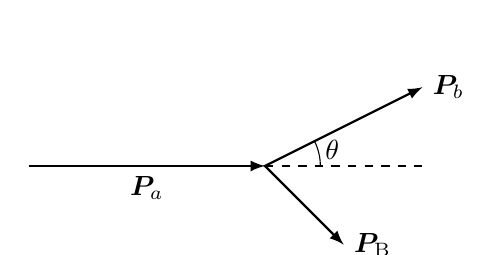
\begin{tikzpicture}
		\coordinate(o)at(0, 0);
		\coordinate(b)at(2, 1);
		\coordinate(c)at(2, 0);
		\coordinate(B)at(1, -1);
		\draw[thick, -latex](-3, 0)--(o)node[midway, below]{$\bm P_a$};
		\draw[thick, latex-latex](B)node[right]{$\bm P_{\nuc B}$}--(o)--(b)node[right]{$\bm P_b$};
		\draw[dashed](o)--(c);
		\pic["$\theta$", draw, angle eccentricity=1.25, angle radius=20]{angle=c--o--b};
	\end{tikzpicture}
	\tikzchap 核反应动量守恒
\end{center}
$b$的出射角$\theta$,由余弦定理,不易测量的$T_\nuc B$可被$P_a,P_b,\theta$表示
\[
	P_\nuc B^2=P_a^2+P_b^2-2P_aP_b\cos\theta.
\]
对于低能核反应,用非相对论公式$P^2=2mT$
%Q=\kh{1+\frac{m_b}{m_{\nuc B}}}T_b-\kh{1-\frac{m_a}{m_{\nuc B}}}T_a-\frac{2\sqrt{m_am_bT_aT_b}}{m_{\nuc B}}\cos\theta
\begin{align}\notag
	Q&=T_b+T_{\nuc B}-(T_a+0)\\
	&=\kh{1+\frac{m_b}{m_{\nuc B}}}T_b-\kh{1-\frac{m_a}{m_{\nuc B}}}T_a-\frac{2\sqrt{m_am_bT_aT_b}}{m_{\nuc B}}\cos\theta
\end{align}
进而可得到出射粒子$b$的能量-角度关系
{\small\begin{align}
	T_b=\hkh{\frac{\sqrt{m_am_bT_a}}{m_{\nuc B}+m_b}\cos\theta\pm\sqrt{\kh{\frac{m_{\nuc B}-m_a}{m_{\nuc B}+m_b}+\frac{m_am_b\cos^2\theta}{(m_{\nuc B}+m_b)^2}}T_a+\frac{m_{\nuc B}}{m_{\nuc B}+m_b}Q}}^2.
\end{align}}
这就是$Q$方程,\index{$Q$方程}将$T_a,T_b,\theta,Q$四个变量联系起来。

当余核B处于激发态的时候,反应能$Q$也会发生相应的改变。

\subsection{核反应的阈值}
\paragraph{实验室系与质心系}
入射粒子$a$和靶核A相对于质心C运动的动能之和,称为$a$的相对运动动能$T'$
\begin{align}
	T'=\frac{m_{\nuc A}}{m_a+m_{\nuc A}}T_a
\end{align}
由于A相对实验室L是静止的,$a$在L系下的动能$T_a$,只有一部分构成了内能项$T'$,能够参与核反应,而整个质心系的动能不能参与核反应。

\paragraph{核反应的阈值}
在L系中能够引起核反应的$a$的最低能量$T_\thres$
\begin{align}
	T_\thres=\frac{m_a+m_{\nuc A}}{m_{\nuc A}}\abs Q.
\end{align}
由于质心系要带走动能,$T_\thres$必然比$\abs Q$大。
\paragraph{出射角转换}
出射粒子在L系和C系中速度的关系
\[
	\bm v_b=\bm v'_b+\bm v\CM
\]
\begin{center}
	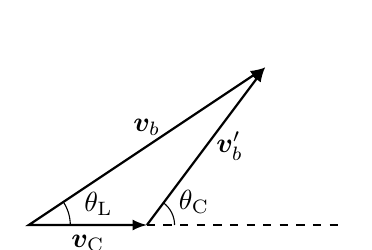
\begin{tikzpicture}
		\coordinate(A)at(0, 0);
		\coordinate(C)at(1.5, 0);
		\coordinate(b)at(3, 2);
		\coordinate(f)at(4, 0);
		% \coordinate(a)at(-1, 0);
		\draw[dashed](C)--(f);
		\draw[thick, -latex](C)--(b)node[midway, right]{$\bm v_b'$};
		\draw[thick, latex-latex](C)--(A)node[midway, below]{$\bm v\CM$}--(b)node[midway, above]{$\bm v_b$};
		\pic["$\theta\LAB$", draw, angle eccentricity=1.75, angle radius=15]{angle=f--A--b};
		\pic["$\theta\CM$", draw, angle eccentricity=1.9, angle radius=10]{angle=f--C--b};
	\end{tikzpicture}
	\tikzchap L系和C系速度关系
\end{center}
由正弦定理、余弦定理等关系
\[
	\begin{cases}
		\frac{v_b'}{\sin\theta\LAB}=\frac{v\CM}{\sin\theta\CM-\sin\theta\LAB}\\
		v_b\cos\theta\LAB=v\CM+v_b'\sin\theta\CM\\
		v_b^2=v\CM^2+v_b'^2+2v\CM v_b'\cos\theta\CM
	\end{cases}
\]
定义
\begin{align}
	\gamma:=\frac{v\CM}{v_b'}.
\end{align}
则
\begin{align}
	\begin{cases}
		\theta\CM=\theta\LAB+\arcsin(\gamma\sin\theta\LAB)\\
		\cos\theta\LAB=\frac{\gamma+\cos\theta\CM}{(1+\gamma^2+2\gamma\cos\theta\CM)^{1/2}}
	\end{cases}
\end{align}
不难用$T'$和$Q$解出$\gamma$
\[
	\gamma^2=\frac{m_am_b}{m_\nuc Am_\nuc B}\frac{m_b+m_\nuc B}{m_a+m_\nuc A}\frac{T'}{T'+Q}
\]
由于$m_a+m_\nuc A\doteq m_b+m_\nuc B$
\begin{align}
	\gamma\doteq\sqrt{\frac{m_am_b}{m_\nuc Am_\nuc B}\frac{T'}{T'+Q}}.
\end{align}
\subparagraph{弹性散射}$Q=0,a=b,\nuc A=\nuc B$,故 
\[
	\gamma=\frac{m_a}{m_\nuc A}.
\]
当$m_\nuc A\gg m_a$时,$\gamma\doteq 0$,$\theta\CM=\theta\LAB$;当$m_\nuc A= m_a$时,$\gamma=1$,$\theta\CM=2\theta\LAB$。
\subparagraph{一般情况}当$\gamma<1$时,$v_b'>v\CM$

当$\theta\CM=\theta\LAB=0$时,$v_b$取最大值$v_{b\max{}}=v_b'+v\CM$;当$\theta\CM=\theta\LAB=\pi$时,$v_b$取最小值$v_{b\min{}}=v_b'-v\CM$。
\begin{center}
	\begin{tikzpicture}
		\coordinate(o)at(0, 0);
		\coordinate(C)at(1.5, 0);
		\coordinate(b)at(3, 2);
		\coordinate(a)at(4, 0);
		\coordinate(d)at(-1, 0);
		\draw[dashed](C)circle(2.5);
		\draw[-latex](C)--(b)node[midway, right]{$\bm v_b'$};
		\draw[latex-latex](C)--(o)node[midway, below]{$\bm v\CM$}--(b)node[midway, above]{$\bm v_b$};
		\draw[red, thick, -latex](o)--(a)node[right]{$v_{b\max{}}$};
		\draw[blue, thick, -latex](o)--(d)node[left]{$v_{b\min{}}$};
		\pic["$\theta\LAB$", draw, angle eccentricity=1.75, angle radius=15]{angle=a--o--b};
		\pic["$\theta\CM$", draw, angle eccentricity=1.9, angle radius=10]{angle=a--C--b};
	\end{tikzpicture}
	\tikzchap $\gamma<1$
\end{center}

当$\gamma>1$时,$v_b'<v\CM$。会出现圆锥效应:
一个$\theta\LAB$对应两个$\theta\CM$
\[
	\theta_{\mathrm L\max{}}=\arcsin\gamma\iv.
\]
\begin{center}
	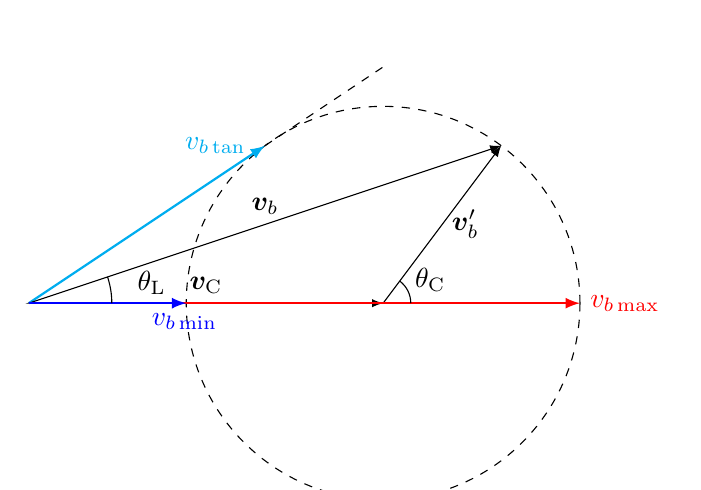
\begin{tikzpicture}
		\coordinate(A)at(-3, 0);
		\coordinate(C)at(1.5, 0);
		\coordinate(b)at(3, 2);
		\coordinate(f)at(4, 0);
		\coordinate(a)at(-1, 0);
		\coordinate(t)at(0, 2);
		\draw[dashed](C)circle(2.5);
		\draw[dashed](t)--(1.5, 3);
		\draw[cyan, thick, -latex](A)--(t)node[left]{$v_{b\tan}~$};
		\draw[-latex](C)--(b)node[midway, right]{$\bm v_b'$};
		\draw[latex-latex](C)--(A)node[midway, above]{$\bm v\CM$}--(b)node[midway, above]{$\bm v_b$};
		\draw[red, thick, -latex](A)--(f)node[right]{$v_{b\max{}}$};
		\draw[blue, thick, -latex](A)--(a)node[below]{$v_{b\min{}}$};
		\pic["$\theta\LAB$", draw, angle eccentricity=1.5, angle radius=30]{angle=f--A--b};
		\pic["$\theta\CM$", draw, angle eccentricity=1.9, angle radius=10]{angle=f--C--b};
	\end{tikzpicture}
	\tikzchap $\gamma>1$圆锥效应
\end{center}

\subsection{核反应截面和产额}
核反应截面$\sigma$的物理意义为一个入射粒子与单位面积上的靶核发生反应的概率。截面的大小与$a,\nuc A$和$T_a$有关。\index{反应截面}

截面的量纲为面积,单位为$\si{barn}$
\begin{align}
	\SI{1}{barn}=\SI{e-24}{cm^2}
\end{align}
与原子核的截面大小相当。

核反应产物的出射可能各向异性,这就会定义微分截面,
\begin{align}
	\sigma(\theta,\phi):=\dv\sigma\Omega(\theta,\phi)
\end{align}
实验测量微分截面,积分可得到总截面。
\[
	\sigma=\int_0^{2\pi}\bs5\int_0^\pi\sigma(\theta,\phi)\sin\theta\d\theta\nd\phi=2\pi\int_0^\pi\sigma(\theta)\sin\theta\d\theta.
\]
\paragraph{反应截面转换}出射粒子数不随坐标系的选择而改变
\[
	\sigma\CM(\theta\CM)\d\Omega\CM=\sigma\LAB(\theta\LAB)\d\Omega\LAB
\]
可得
\[
	\sigma\LAB(\theta\LAB)=\frac{(1+\gamma^2+2\gamma\cos\theta\CM)^{3/2}}{1+\gamma\cos\theta\CM}\sigma\CM(\theta\CM).
\]
\paragraph{核反应产额}定义:入射粒子在靶中引起的核反应数$N'$与入射粒子数$I_0$之比,称为核反应产额(yield) $Y$。\index{反应产额}
\begin{align}
	Y:=\frac{N'}{I_0}.
\end{align}
与反应截面$\sigma$和数密度$N$有关。

通过厚度为$D$的靶后,未发生反应的入射粒子数
\[
	-\frac{\d I}{I}=\sigma N\d x,\thus I=I_0\e{-\sigma ND}
\]
故透射率$T=\e{-\sigma ND},$
\begin{align}
	Y=1-\e{-\sigma ND}.
\end{align}
宏观截面($\si{1/cm}$) $\Sigma:=N\sigma$,平均自由程$\lambda=1/\Sigma$,厚靶$D\gg\lambda,Y=1.$

\subsectionstar{核反应中的分波分析}
尽管核反应截面的单位$\si{barn}$与原子核截面相近,但是有时候二者也可以差异巨大。入射粒子带来的轨道角动量有不同的组成,可以根据不同的轨道角动量来分析核反应截面。

\paragraph{半经典的分波分析}入射粒子$a$速度$v_a$,相对质心的运动动能
\[
	T'=\frac12\mu v_a^2,\quad \mu:=\frac{m_am_{\nuc A}}{m_a+m_{\nuc A}}.
\]
相对运动动量
\[
	p=\mu v_a=\frac\hbar\barlambda,\quad\lambdabar:=\frac\hbar{p}.
\]
式中$\lambdabar$是约化de Broglie波长。\\
相对运动角动量
\[
	L=\rho p=\frac\rho\barlambda\hbar=\ell\hbar,\thus\rho=\ell\lambdabar,\quad\ell=0,1,\ldots
\]%ħ

$(a,\nuc A)$的碰撞过程,可以被分解为对应于轨道角动量$L=0,\hbar,2\hbar,\ldots$的部分。轨道角动量为$\ell\hbar$的入射粒子与靶核作用的截面为
\[
	S_\ell=\pi(\rho_{\ell+1}^2-\rho_\ell^2)=(2\ell+1)\pi\lambdabar^2.
\]
最大半径$\rho\maxi=R=R_a+R_{\nuc A}$,进而得到反应截面
\begin{align}
	\sigma=\sum_{\ell=0}^{R/\barlambda}(2\ell+1)\pi\lambdabar^2=\pi(R^2+\lambdabar^2),
\end{align}
核的尺寸和粒子的波动性,都对截面有贡献。
\paragraph{量子力学的分波分析}
向$x$方向入射的粒子束可用平面波表示,在有心力场中,球面波分解更合适
\[
	\psi_\i=\e{\i kx}=\e{\i kr\cos\theta}=\sum_{\ell=0}^\infty(2\ell+1)\i^\ell j_\ell(kr)P_\ell(\cos\theta),
\]
波函数远离原子核时,$kr\gg\ell$,
\[
	j_\ell(kr)\doteq\frac{\sin(kr-\pi\ell/2)}{kr}=\i\frac{\e{-\i(kr-\pi\ell/2)}-\e{\i(kr-\pi\ell/2)}}{kr}.
\]
故
\[
	\psi_\i=\frac1{2kr}\sum_{\ell=0}^\infty\i^{\ell+1}(2\ell+1)\fkh{\e{-\i(kr-\pi\ell/2)}-\e{\i(kr-\pi\ell/2)}}P_\ell(\cos\theta).
\]
其中$\e{-\i(kr-\pi\ell/2)}$代表入射球面波,$\e{\i(kr-\pi\ell/2)}$代表出射球面波。
由于原点上有靶核,散射会导致出射波函数的变化,
\[
	\psi=\frac1{2kr}\sum_{\ell=0}^\infty\i^{\ell+1}(2\ell+1)\fkh{\e{-\i(kr-\pi\ell/2)}-\eta_\ell\e{\i(kr-\pi\ell/2)}}P_\ell(\cos\theta).
\]
其中$\eta_\ell$是出射波系数。
故靶核导致的散射
\begin{align}
	\psi_\sca=\psi-\psi_\i=\frac1{2kr}\sum_{\ell=0}^\infty\i^{\ell+1}(2\ell+1)(1-\eta_\ell)\e{\i(kr-\pi\ell/2)}P_\ell(\cos\theta).
\end{align}

散射截面等于散射粒子数比上入射粒子注量率,因此
\[
	\d\sigma_\sca=\frac{j_\sca r^2\d\Omega}{j_\i},
\]
量子力学中
\[
	j=\frac{\hbar}{2m\i}\kh{\psi\cj\pv\psi{r}-\psi\pv{\psi\cj}r}.
\]
以$\ell=0$为例,计算得到
\[
	j_\sca=\frac{\hbar k}m\frac{\abs{1-\eta_0^2}}{4k^2r^2},\quad j_\i=\frac{\hbar k}m.
\]
故
\[
	\dv{\sigma_{\mathrm{sc},0}}\Omega=\frac{\abs{1-\eta_0^2}}{4k^2}=\frac{\barlambda^2}4\abs{1-\eta_0^2},
\]
把所有角动量均考虑进去
\[
	\dv{\sigma_\sca}\Omega=\frac{\barlambda^2}4\abs{\sum_{\ell=0}^\infty\i(2\ell+1)(1-\eta_\ell)P_\ell(\cos\theta)}^2.
\]
对$4\pi$立体角积分得散射截面
\begin{align}
	\sigma_\sca=\pi\lambdabar^2\sum_{\ell=0}^\infty(2\ell+1)\abs{1-\eta_\ell}^2.
\end{align}
对于反应截面,可以认为$a$消失了,类似的推导得出
\[
	\sigma_{\mathrm{r}}=\pi\lambdabar^2\sum_{\ell=0}^\infty(2\ell+1)(1-\abs{\eta_\ell}^2).
\]

\paragraph{低能中子的散射截面}对于低能入射中子,$\ell=0$,波函数简化为 
\[
	u_{\mathrm o}(r)=\frac\i{2k}\kh{\e{-\i kr}-\eta_0\e{\i kr}}.
\]
若入射粒子与核的作用已知,则核内波函数可知,继而可知核边界处的对数导数
\[
	f:=\edg{\frac r{u_{\mathrm o}}\dv{u_{\mathrm o}}r}_{r=R}\thus\eta_0=\frac{f+\i kR}{f-\i kR}\e{-\i2kR}
\]
当$f\to\infty$时,$\eta=\e{-\i2kR}$;当$f\to0$时,$\eta=-\e{-\i2kR}$,慢中子$kR\ll 1$,故 
\begin{align}
	\sigma_{\mathrm{sc},0}=\begin{cases}
		4\pi R^2,&f\to\infty\\
		4\pi\lambdabar^2,&f\to0
	\end{cases}
\end{align}
$4\pi R^2$对应势(形状)弹性散射截面,$4\pi\lambdabar^2$对应共振散射截面。
\paragraph{散射截面vs反应截面}
\begin{center}
	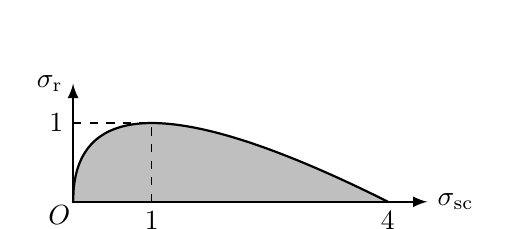
\begin{tikzpicture}
		\draw[thick, domain=0:4, samples=500, fill=gray!50]plot(\x, {2*sqrt(\x)-\x})node[below]{4};
		\coor{4.5}{1.5}{\sigma_\sca}{\sigma_\mathrm r};
		\draw[dashed](0, 1)node[left]{1}--(1, 1)--(1, 0)node[below]{1};
	\end{tikzpicture}
	\tikzchap 散射截面$\sigma_\sca$与反应截面$\sigma_\mathrm r$的允许范围
\end{center}
允许有纯的散射过程($|\eta_\ell|=1$),但不允许有纯的反应过程。入射道对出射道总是开放的——入射粒子可以沿入射道返回,因此一定存在弹性散射。
\subsection{核反应机制及核反应模型}
\paragraph{核反应的三阶段描述}Weisskopf将核反应分为了三个阶段:
\begin{compactenum}
	\item \textbf{独立粒子阶段}:
	
	部分入射粒子被吸收,引起核反应;\\
	部分入射粒子被散射,形成弹性散射
	\item \textbf{复合系统阶段}:
	
	入射粒子与靶核交换能量:
	直接作用;形成复合核;中间过程
	\item \textbf{最后阶段}:
	
	复合系统分解为出射粒子和剩余核。
\end{compactenum}
各种截面有关系,间讲义。
\paragraph{复合核模型}核反应被分成相互独立的两个阶段:
\[
	a+\nuc A\to\nuc C^\ast\to\nuc B+b
\]
\begin{compactenum}
	\item 入射粒子射入靶核,与之形成一个复合核,该核处于激发态;
	\item 激发态的复合核可沿入射道弹性散射,也可能开放其它反应道。
\end{compactenum}
复合核的激发能$E^\ast$是相对动能$T'$和结合能$B_{a\nuc A}$的和
\begin{align}
	E^\ast=T'+B_{a\nuc A}=\frac{m_\nuc A}{m_a+m_\nuc A}T_a+B_{a\nuc A}.
\end{align}
复合核发射核子一般需要$\sim\SI{8}{MeV}$的分离能。尽管$E^\ast\sim\SI{20}{MeV}$,但平均到每个核子的能量只有$\SI{0.2}{MeV}$,故复合核的分离需要经过多次碰撞,其寿命$\sim\SIrange{e-18}{e-14}{s}$,对核反应而言,这是较长的时间。

反应截面
\begin{align}
	\sigma_{ab}=\sigma_{\mathrm{CN}}(T_a)W_b(E^\ast),
\end{align}
故复合核如何衰变是与它如何形成无关,只取决于系统现在的能量状态。
\paragraph{共振}只考虑s波,即$\ell=0$的情况,$\eta_0=\e{\i2\delta_0}$
\[
	\sigma_{\mathrm{sc},0}=\pi\lambdabar^2|1-\eta_0|^2=4\pi\lambdabar^2\sin^2\delta_0(T').
\]
当入射中子的能量达到某些值时,$\delta_0(T')=\pi/2$,散射截面达到极大,就出现了共振。

在$\delta_0(T')=\pi/2$处($T'=E_\mathrm R$)做Talyor展开,略去高阶项
\[
	\sigma_{\mathrm{sc},0}=\pi\lambdabar^2\frac{\Gamma^2}{(T'-E_\mathrm R)^2+\Gamma^2/4}.
\]
势弹性散射和共振弹性散射是复数和的关系,因此存在干涉。
\paragraph{慢中子反应}对于慢中子与一个$A>100$的靶核而言,最可几的复合核退激机制是发射$\gamma$射线,$(\nton,\gamma)$反应是个比较慢的过程
\[
	\sigma_{\nton,\gamma}=\pi\lambdabar^2\frac{\Gamma_\nton\Gamma_\gamma}{(T'-E_\mathrm R)^2+\Gamma^2/4}.
\]
由于约化de Broglie波长
\[
	\lambdabar^2=\frac{\hbar^2}{2\mu T'^2}\propto\frac1{v^2}
\]
低能中子进入势阱,$E_\nton\ll V_0$,并不容易
\[
	P\propto k\propto v,\thus\Gamma_\nton\propto v
\]

慢中子的动能,对衰变行为没什么影响,$T'\ll B_{\nton\nuc A}$,故
\[
	E^\ast=\cns,\enspace\Gamma_\gamma=\cns
\]

非共振中子,能量的变化对复合核的衰变不再有什么影响了$\Gamma=\Gamma_\nton+\Gamma_\gamma$,$\Gamma_\nton\ll\Gamma_\gamma$,$\Gamma=\cns$,故\index{$1/v$规律}
\begin{align}\label{slow-neutron}
	\sigma_{\nton,\gamma}\propto\frac1v.
\end{align}
当我们用慢中子来照射靶核时,中子能量的降低将会有助于$(\nton,\gamma)$反应的发生,该反应的截面反比于中子的速度。

这里的讨论是在“中子能量远离共振能量”这个前提下开展的,如果中子的动能碰巧在共振能量附近,则公式中分母的第一项会起作用,使的截面或大或小的偏离$1/v$规律
\paragraph{连续区理论}连续区——$T'$增加,复合核处于高激发态,能级重叠。能级密度加大,能级宽度加大,不再有单能级共振。
\paragraph{总结}截面测量
\clearpage
\sectionstar{裂变和聚变}
不讲
\clearpage
\section{辐射与物质的相互作用}
\begin{definition}{致电离辐射}{ionizing radiation}
	能直接或间接导致原子或分子电离的辐射。比如$\alpha,\beta,\pton,$重离子, $\pi$介子, $\mu$子……
\end{definition}
致电离辐射要求能量足够大,一般大于$\SI{10}{eV}$。但是中子有$\si{MeV}$级能量的$B_{\nton\nuc A}$,因此低能中子仍可致电离。
\begin{center}
	\begin{tikzpicture}
		\node at(0, 5){直接致电离辐射};
		\node at(7, 5){间接致电离辐射};
		\node(e)at(0,4){快电子};
		\node(X)at(7,4){电磁辐射X,$\gamma$};
		\node(C)at(0,0){重带电粒子};
		\node(n)at(7,0){中子};
		\draw[thick,-latex](X)--(e)node[midway,above]{次级电子}node[midway, below]{光原子反应};
		\draw[thick, -latex](n)--(X)node[midway, right]{原子核(n,$\gamma$)};
		\draw[thick, -latex](n)--(C)node[midway,above]{次级重带电粒子}node[midway, below]{核反应(n,c) (n,f)};
		\draw[thick, -latex](n)--(e)node[midway, sloped, above]{核反应之后的内转换电子};
	\end{tikzpicture}
	\tikzchap 致电离辐射的种类
\end{center}
\paragraph{弹性碰撞和非弹性碰撞}
\[
	\frac12mv^2+\frac12MV^2=\frac12mv'^2+\frac12MV'^2+\D E.
\]
$\D E=0$为弹性碰撞;$\D E>0$为第一类非弹性碰撞,使处于基态的原子激发或者电离;$\D E<0$为第二类非弹性碰撞,使处于激发态的原子退激。
\paragraph{带电粒子在物质中的慢化}
\begin{compactenum}
	\item 电离损失:带电粒子与靶原子核外电子的非弹性碰撞,包括电离和激发导致的能损;
	\item 辐射损失:带电粒子与靶原子核的非弹性碰撞,产生的电磁辐射被称为\textbf{轫致辐射}(bremsstrahlung, 车字旁);
	\item 核阻止:带电粒子与靶原子核的弹性碰撞;
	\item 带电粒子与核外电子的弹性碰撞。
\end{compactenum}
其中电离损失和辐射损失是主要的能量损失方式,二者之间是竞争关系。\textbf{对于重带电粒子,电离损失重要;对于电子,辐射损失重要。}
\subsection{重带电粒子与物质的相互作用}
重带电 粒子一般为正电荷,主要通过电离损失的方式来损失能量,使介质电离或激发,在介质中的运动轨迹近似为直线。
\begin{definition}{能量损失率}{}
	能量损失率是单位路径上引起的能量损失,又称比能损失或阻止本领
	\begin{align}
		S:=-\dv Ex.
	\end{align}
	按照能量损失作用的不同,能量损失率可分为:电离能量损失率、辐射能量损失率和核碰撞能量损失率。
\end{definition}
\subsubsection{Bethe公式}
重离子的能量损失率主要是电离能量损失率$S_{\mathrm{ion}}$。
1930年,Bethe提出了描述电离能量损失率$S_{\mathrm{ion}}$与带电粒子速度$v$、电荷$z$等关系的经典公式。

公式推导的简化条件:
\begin{compactenum}
	\item 物质原子的电子可以看成是自由、静止的;
	\item 入射带电粒子碰撞后仍按原方向运动;
	\item 入射带电粒子的电荷量保持不变
\end{compactenum}

先考虑入射粒子与电子的相互作用:在$x$方向,电子获得的动量为0,$y$方向动量 
\[
	p_y=\int\iti\frac{ze^2}{4\pi\varepsilon_0r^2}\frac br\frac{\d x}v=\frac{ze^2b}{4\pi\varepsilon_0v}\int\iti\frac{\d x}{r^3}=\frac1{4\pi\varepsilon_0}\frac{2ze^2}{bv}.
\]
碰撞参数为$b$的单个电子所获得的动能为
\[
	\D E(b)=\frac{p_y^2}{2m_\elc}=\kh{\frac1{4\pi\varepsilon_0}}^2\frac{2z^2e^4}{m_\elc v^2b^2}.
\]
碰撞参数为$b$的电子数为
\[
	NZ\cdot 2\pi b\d b\nd x.
\]
其中$N$为介质的原子数密度,$Z$是介质的原子序数。
\newpage
$\d x$距离内,物质中所有电子得到的总能量为
\[
	-\d E=\frac{e^4}{4\pi\varepsilon_0^2}\frac{NZ\d x}{m_\elc}\frac{z^2}{v^2}\int_{b\mini}^{b\maxi}\frac{\d b}b.
\]
$b\mini$对应电子获得最大能量的情况:按经典碰撞理论,重离子与电子对心碰撞时,电子将获得最大动能
\[
	\D E(b\mini)=\frac12m_\elc(2v)^2,\thus b\mini=\frac1{4\pi\varepsilon_0}\frac{ze^2}{m_\elc v^2}.
\]
$b\maxi$对应电子获得最小能量的情况。为了电离或者激发电子,入射粒子传给电子的能量必须大于物质原子中电子的激发能$I$
\[
	\D E(b\maxi)=I,\thus b\maxi=\frac1{4\pi\varepsilon_0}\frac{ze^2}{v^2}\sqrt{\frac2{m_\elc I}}.
\]
\begin{example}{}{}
	$\SI{4}{MeV}$的$\alpha$粒子射入一个平均电离能为$\SI{10}{eV}$的物质,
	\[
		b\maxi=\SI{3.89e-11}{m},\quad b\mini=\SI{2.63e-12}{m}
	\]
\end{example}

代入$b\maxi,b\mini$,得到Bethe-Bloch公式
\begin{align}\label{Bethe-formula}
	S_{\mathrm{ion}}=\frac{e^4}{4\pi\varepsilon_0^2}\frac{NZ}{m_\elc}\frac{z^2}{v^2}B,
\end{align}
其中 
\[
	B=\frac12\ln\biggkh{\frac{2m_\elc v^2}I}.
\]
Bethe考虑相对论与其他修正因子,得到精确表达式(略)。
%$B=\ln\kh{\frac{2m_\elc v^2}I}-\ln\kh{1-\frac{v^2}{c^2}}-\frac{v^2}{c^2}.$


对于介质,
\begin{align}
	S_{\mathrm{ion}}\propto NZ,
\end{align}
说明吸收材料电子密度大的,阻止本领大;

对于入射带电粒子(非相对论情况下,$B$随$v$变化缓慢),
\begin{align}
	S_{\mathrm{ion}}\propto\frac{z^2}{v^2}.
\end{align}
与其质量$m$无关,仅与其速度$v$和电荷数$z$有关。
\newpage
实际电离能量损失率随粒子的平均核子能量$E/A$变化会有三段:
\begin{compactenum}
	\item $E/A<500I(\sim\SI{30}{keV})$,入射粒子能量很低,入射粒子容易从靶物质中拾取电荷,有效电荷降低;
	\item $500I<E/A<\SI{1.5}{GeV}$,$S_{\mathrm{ion}}\propto1/E$;
	\item $E/A>\SI{1.5}{GeV}$,相对论效应起作用。
\end{compactenum}
$S_{\mathrm{ion}}$的极小值出现在$3m_\pton c^2(\sim\SI{3}{GeV})$附近,对应平均核子能量的粒子\footnote{若粒子不由核子组成,比如能量为$3m_\elc c^2$的电子或$3m_\mu c^2$的$\mu$子也是MIPs。}称为最小电离粒子(minimum ionizing particles, MIPs)

单位电荷的带电粒子,在穿透了介质的单位质量厚度后的能量损失为:
\[
	\frac{S_{\mathrm{ion}}}{\rho z^2}\propto\frac{e^4}{4\pi\varepsilon_0^2}\frac{1}{m_\elc}\frac{1}{v^2}B,
\]
因此不同粒子$S_{\mathrm{ion}}/\rho z^2\vs E/A$的曲线在高能处基本重合,极小值(MIPs)是相同的
\[
	\sim\frac{\SI{1.8}{MeV}}{\si{g/cm^2}}.
\]
$Z$大的核,在低能时更容易吸附电子,导致$Z$下降,曲线下降。
\subsubsection{重带电粒子的径迹与射程}
\paragraph{Bragg曲线}带电粒子的能量损失率沿其径迹的变化曲线。

%$\SI{1}{MeV}$质子在水中不同位置处沉积的能量,
根据Bethe公式,$S_{\mathrm{ion}}$会先因为$v$降低而逐渐上升($1/v^2$),在$v$足够低时因为吸收电荷导致$z$降低而迅速下降($z^2$)。

应用:重离子治疗。
\paragraph{粒子径迹的特征}重带电粒子在物质中径迹的特征?
\begin{compactenum}
	\item 基本是直线,有分叉;
	\item $\alpha$比p粗;
	\item 能量越高越细。
\end{compactenum}
\begin{definition}{比电离}{specific ionization}
	带电粒子在穿透单位距离介质时产生的平均电子-离子对数。
\end{definition}
$\delta$射线:带电粒子穿透介质时所产生电子-离子对中的高能量、 可引起进一步电离的电子。
\paragraph{粒子的射程与定比定律}带电粒子沿入射方向行经的最大距离,称为入射粒子在该物质中的射程$R$。

重带电粒子由于质量大,与物质原子相互作用时,其运动方向几乎不变,射程与实际路程相近。

\begin{example}{$\alpha$粒子射程经验公式}{}
	$\SI{15}{\celsius}$和$\SI{1}{atm}$下$\alpha$粒子的射程满足
	\[
		R=0.318E_\alpha^{3/2}\,\si{cm}.
	\]
	适用范围$\SIrange{3}{7}{MeV}$
\end{example}
可以由能量损失率求出射程
\begin{align}
	R=\int_0^{E_0}-\frac{\d E}{S_{\mathrm{ion}}}=4\pi\varepsilon_0^2\frac{m_\elc m}{z^2e^4NZ}\int_0^{v_0}\frac{v^3}B\d v\propto E^2.
\end{align}
由上式,同一吸收物质中,初速度相同的不同重带电粒子的射程之间的关系
\begin{align}
	R\propto\frac{m}{z^2},%F(v),\quad F(v):=\frac{4\pi\varepsilon_0^2m_\elc}{e^4NZ}\int_0^{v_0}\frac{v^2}B\d v
\end{align}
高能区能量损失率几乎不变,
\[
	R\propto E.
\]



阻止时间:将带电粒子阻止在吸收体内所需的时间。对非相对论粒子
\[
	v=\sqrt{\frac{2E}{m}}=c\sqrt{\frac{2E}{mc^2}},\quad\avg v=kv.
\]
取$k=0.6$,则
\[
	T=\frac{R}{\avg v}=\frac{R}{kc}\sqrt{\frac{mc^2}{2E}}=\num{1.2e-7}R\sqrt{\frac{m}E}.
\]
$m$的单位为u,$E$的单位为MeV,$R$单位为m,$t$单位为s。
数MeV $\alpha$粒子的阻止时间:气体$\sim\si{ns}$,固体$\sim\si{ps}$
\paragraph{在薄吸收体中的能量损失}
带电粒子在薄吸收体中的能量损失
\[
	\D E=\avg SD.
\]
如果是较厚的吸收体,则需要借助“能量-射程”曲线
\paragraph{能量歧离和射程歧离}
碰撞电离是个随机过程,单能粒子穿过一定厚度的物质后,将不再是单能的(对一组粒子而言),而发生了能量和射程的涨落,这就是能量/射程歧离(energy/range straggling)。
\paragraph{裂变碎片的能量损失}
裂变碎片是核裂变所产生的重带电粒子,电荷量大,质量大。裂变碎片的能量损失率很大,射程很短,约为$\SI{5}{MeV}\,\alpha$粒子的一半。
\subsection{快电子与物质的相互作用}
\begin{center}
	\begin{tabular}{ccc}
		\toprule
		&重带电粒子&快电子\\
		\midrule
		质量&大&小\\
		速度&小&大\\
		能量损失方式&电离&电离、辐射\\
		径迹特性&直线&曲折、散射严重\\
		\bottomrule
	\end{tabular}
\end{center}
\paragraph{快电子的能量损失率}
快电子的电离能量损失和辐射能量损失都很重要,同时,需要考虑相对论效应。

电离能量损失:电子的Bethe公式为
\begin{align}
	S_{\mathrm{ion}}=\frac{e^4}{8\pi\varepsilon_0^2}\frac{NZ}{m_\elc}\frac{1}{v^2}B,
\end{align}
相较而言,电子是弱电离粒子。

辐射能量损失:带电粒子穿过物质时,受原子核Coulomb场的影响,其速度发生变化,会伴随发射电磁波,即轫致辐射。量子电动力学计算表明,辐射能量损失率服从:
\begin{align}
	S_{\mathrm{rad}}\propto\frac{z^2E}{m^2}NZ^2.
\end{align}
快电子的两种能量损失率之比
\begin{align}
	\frac{S_{\mathrm{rad}}}{S_{\mathrm{ion}}}\doteq\frac{EZ}{\SI{800}{MeV}}.
\end{align}
探测学中所涉及快电子的能量$E\sim\si{MeV}$,所以辐射能量损失仅在高$Z$吸收材料中才是重要的。

当要吸收、屏蔽$\beta$射线时,不宜选用重材料,应该用轻材料;
当要获得强的X射线时,则应选用重材料作靶。

\paragraph{电子的吸收、散射和$\beta$射线的射程}
由于单能电子和$\beta$粒子易受散射,其吸收衰减规律不同于$\alpha$粒子,但均存在最大射程$R\maxi$。射程往往通过实验测定。

初始能量相等的电子在各种材料中的射程与吸收体密度的乘积近似为常数
\[
	R\maxi \rho=R_m(E)
\]
\begin{center}
	\tablechap{典型物质中$\beta$射线的射程 }
	\begin{tabular}{ccc}
		\toprule
		物质&射程&单位\\
		\midrule
		Ge&$R\sim E_{\beta\max{}}$&$\si{mm},\si{MeV}$\\
		Al&$R\sim 2E_{\beta\max{}}$&$\si{mm},\si{MeV}$\\
		Air&$R\sim 400E_{\beta\max{}}$&$\si{cm},\si{MeV}$\\
		\bottomrule
	\end{tabular}
\end{center}
$\SI{4}{MeV}$的$\alpha$粒子在空气中的射程约为$\SI{2.5}{cm}$;

电子与靶物质原子核Coulomb场作用时,只改变运动方向,而不辐射能量的过程称为弹性散射。由于电子质量小,因而散射的角度可以很大,而且会发生多次散射,最后偏离原来的运动方向,电子沿其入射方向发生大角度偏转,称为反散射(backscatter)。只在电子能量很小($\SI{100}{eV}$)时才需要考虑。定义反散射系数
\[
	\eta=\frac{I_{\mathrm{bs}}}{I_0},
\]
从实验曲线看出:
\begin{compactenum}
	\item 同种材料:入射电子能量越低,反散射越严重;
	\item 同样能量的入射电子:原子序数越高的材料,反散射越严重;
	\item 低能电子在高原子序数的厚样品物质上的反散射系数可达50\%。
\end{compactenum}
对放射源而言,利用反散射可以提高$\beta$源的产额,给源加一个高$Z$厚衬底;对探测器而言,要避免反散射造成的测量偏差,使用低$Z$材料作探测器及其入射窗。
\paragraph{正电子与物质的相互作用}
正电子与电子以同样的机制来损失能量。
但是在径迹末端的表现不同:
\begin{compactitem}
	\item 正电子在径迹末端与介质中的电子湮没(annihilation),放出$\gamma$光子;
	\item 或者与一个电子结合成正电子素(电子偶素,positronium),即电子-正电子对的束缚态($^1$S反平行或$^3$S平行),然后再湮没,放出$\gamma$光子。
\end{compactitem}

正电子湮没时一般放出两个光子,两个湮没光子的能量相同,方向相反,平均来看各向同性出射。\footnote{Doppler效应可能导致偏离$180^\circ$。}

湮没还可以放出三个光子,概率仅为放出两个光子概率的1/370;
还可以发生单光子湮没\footnote{if the negative electron is bound to a nucleus.},但是概率要更低,$~\sim(\alpha Z)^4$ 4个量级。

正电子在高速时也可以湮没,但截面较小。

慢化后正电子在材料中单位时间发生湮没的概率:
\[
	P=\pi r_\elc^2cn,
\]
$r_\elc$是经典电子半径
\[
	r_\elc=\frac{e^2}{4\pi\varepsilon_0}\frac1{m_\elc c^2}.
\]
$n$是材料中的电子密度,故正电子的寿命
\[
	\tau=\frac1P=\num{2.21e-10}\frac{A}{\rho Z}\,\si{s}.
\]
\subsection[\textit{\textgamma}射线与物质的相互作用]{$\gamma$射线与物质的相互作用}
探测学中,$\gamma$射线有核能级跃迁产生的特征$\gamma$射线,和正电子湮没产生$\SI{511}{keV}$的湮没辐射;X射线有原子能级跃迁产生的特征X射线,也有带电粒子变速时产生的轫致辐射。$\gamma$射线和X射线本质是一样的,与物质发生相互作用的规律也是一样的。

$\gamma$射线可以和物质发生多种相互作用:
\begin{compactitem}
	\item 光与原子核:光核反应;
	\item 光与自由电子:Thomson散射;
	\item 光与原子:光电效应,Compton散射,电子对效应,Rayleigh散射,Raman散射。
\end{compactitem}
这些相互作用的截面大小是不同的。

对于keV - MeV的$\gamma$射线,最主要的三种光原子反应类型是:光电效应、Compton散射和电子对效应。此外,在考虑射线衰减时,也要考虑Rayleigh散射。
\subsubsection{光电效应}
光子把全部能量传递给原子的某个束缚电子,使之发射出去成为光电子(photoelectron),而光子本身消失,原子被电离并略有反冲的过程的过程。其特点为:
\begin{compactenum}
	\item 是与束缚电子,而非自由电子发生相互作用。
	\item 主要与原子中结合的最紧的K层电子发生作用,K层电子的光点截面大约占了光点效应总截面的80\%。
	\item 光电效应发生后,内层电子出现空位,将有后续的退激过程。
\end{compactenum}
光电子能量 
\[
	E_\elc=h\nu-\varepsilon_i.
\]
光电效应的微分截面
\[
	\dv{\sigma_{\mathrm{ph}}}\Omega\propto Z^5\kh{\frac{m_\elc c^2}{h\nu}}^{7/2}\frac{\sin^2\theta\cos^2\phi}{(1-\beta\cos\theta)^4}.
\]
\begin{compactenum}
	\item 在$\theta=0^\circ$和$\theta=180^\circ$方向没有光电子飞出;
	\item 入射光子能量低时,光电子趋于垂直方向发射;
	\item 入射光子能量较高时,光电子趋于向前发射。
\end{compactenum}

但并不是任何电子都可以参与光电效应,对于$h\nu<\SI{100}{eV}$的$\gamma$光子,截面会在吸收限(absorption edge) $\varepsilon_\mathrm K,\varepsilon_\mathrm L,\ldots$等处出现阶跃。

光电效应后续会出现特征X射线和Auger电子,结合能高时前者占优。

\subparagraph{总结}
对于$\gamma$光子的测量来说,光电效应可说是最重要的反应类型了!因为它可以“最有效地”把光子的能量转换为光电子的动能,由后者在探测器内形成信号,使能谱中出现\textbf{光电峰}。

光电效应是一个很容易提升截面的效应
\begin{align}
	\sigma_{\mathrm{ph}}\propto Z^5.
\end{align}
与吸收材料的$Z$密切相关。探测中采用高$Z$材料,可提高探测效率;屏蔽中采用高$Z$材料,可以有效阻挡$\gamma$射线。

$\gamma$光子能量$h\nu$越高,光电效应截面$\sigma_{\mathrm{ph}}$越小。
\subsubsection{Compton散射}
1922年,美国物理学家Compton在研究X射线与物质散射的实验里,发现了Compton散射。

Compton散射:是光子与核外电子的非弹性碰撞过程。特点:
\begin{compactenum}
	\item 入射光子的部分能量转移给电子,使其电离成为反冲电子;
	\item 光子受到散射,方向和能量都发生变化,称为散射光子;
	\item 主要与外层电子发生Compton散射。
\end{compactenum}
讨论Compton散射是从光子与自由(电离能很小)静止(轨道电子速度$\ll c$)电子的散射开始的
\paragraph{散射光子、反冲电子的能量-角度关系}由能量守恒和动量守恒
\begin{align*}
	h\nu+m_\elc c^2&=h\nu'+\sqrt{(m_\elc c^2)^2+(p_\elc c)^2},\\
	\frac{h\nu}c&=\frac{h\nu'}c\cos\theta+p_\elc\cos\varphi,\\
	0&=\frac{h\nu'}c\sin\theta-p_\elc\sin\varphi.
\end{align*}
有$\nu',p_\elc,\theta,\varphi$ 4个变量,故散射光子和反冲电子的能量是连续的,确定一个变量,得到
\begin{align}\label{Compton-hnu}
	h\nu'=\frac{h\nu}{1+\alpha(1-\cos\theta)},\quad \alpha:=\frac{h\nu}{m_\elc c^2},
\end{align}
$\theta=0$时,$h\nu'=h\nu$最大;$\theta=180^\circ$时,$h\nu'$最小。当光子发生大角度($\theta>150^\circ$)散射时,$E_\elc$随$\theta$的变化很慢,就导致了\textbf{反散射峰}的出现——$\gamma$能谱中的一个著名本底峰。

当$h\nu\gg m_\elc c^2$时,$h\nu'$的最小值
\[
	h\nu'=\frac12m_\elc c^2=\SI{255}{keV};
\]
当$h\nu\ll m_\elc c^2$时,$h\nu'\doteq h\nu$,变成Thomsom散射。

将式(\ref{Compton-hnu})改写为波长的形式,得到Compton移动
\begin{align}
	\D\lambda=\frac h{m_\elc c}(1-\cos\theta).
\end{align}

散射角与反冲角存在一一对应的关系
\[
	\cot\varphi=(1+\alpha)\tan\frac\theta{2}.
\]

\paragraph{散射截面和角分布}
Klein-Nishina公式:
\begin{align*}
	\dv{\sigma_{\mathrm C,\elc}}\Omega&=\frac{r_\elc^2}2\kh{\frac{\nu'}\nu}^2\kh{\frac{\nu'}\nu+\frac\nu{\nu'}-\sin^2\theta}
	%\\&=\frac{r_\elc^2}2(1+\cos^2\theta)\fkh{\frac1{1+\alpha(1-\cos\theta)}}^2\fkh{1+\frac{\alpha^2(1-\cos\theta)^2}{(1+\cos^2\theta)\bigfkh{1+\alpha(1-\cos\theta)}}}.
\end{align*}
角分布
\[
	\dv{\sigma_{\mathrm C,\elc}}\theta=\dv{\sigma_{\mathrm C,\elc}}\Omega\dv\Omega\theta=2\pi\sin\theta\cdot\dv{\sigma_{\mathrm C,\elc}}\Omega.
\]
\paragraph{反冲电子角分布和能量分布}
反冲电子能量和方向与散射光子能量和方向一一对应,可以推出反冲电子的微分散射截面
\[
	\dv{\sigma_{\mathrm C,\elc}}{\Omega'}=\dv{\sigma_{\mathrm C,\elc}}\Omega\frac{\sin\theta\d\theta}{\sin\varphi\d\varphi}=\frac{(1+\alpha)^2(1-\cos\theta)^2}{\cos^2\varphi}\dv{\sigma_{\mathrm C,\elc}}\Omega.
\]
反冲电子能量分布
\[
	\dv{\sigma_{\mathrm C,\elc}}{E_\elc}=\dv{\sigma_{\mathrm C,\elc}}\Omega\dv\Omega\theta\dv\theta{E_\elc}=\frac{2\pi m_\elc c^2}{(h\nu-E_\elc)^2}\dv{\sigma_{\mathrm C,\elc}}\Omega.
\]
即
\[
	\dv{\sigma_{\mathrm C,\elc}}{E_\elc}=\pi r_\elc^2\cdot\frac{m_\elc c^2}{(h\nu)^2}\fkh{2+\kh{\frac{E_\elc}{h\nu-E_\elc}}^2\kh{\frac1{\alpha^2}-\frac{2(h\nu-E_\elc)}{\alpha E_\elc}}+\frac{h\nu-E_\elc}{E_\elc}}.
\]
微分截面 - 反冲电子能量会呈现一个逐渐缓慢上升然后突然下降的形状,称之为Compton坪和Compton边缘。考虑原子外电子(非自由电子)的结合能时,就需要考虑Doppler效应,Compton边缘将不再锐利。Compton坪对$\gamma$能谱的解读而是很不利的。

\paragraph{总截面}单个电子的Compton散射总截面
\begin{align*}
	\sigma_{\mathrm C,\elc}&=\int_0^\pi\dv{\sigma_{\mathrm C,\elc}}\theta\d\theta\\
	&=2\pi r_\elc^2\fkh{\frac{\alpha^3+9\alpha^2+8\alpha+2}{\alpha^2(1+2\alpha)^2}+\frac{\alpha^2-2\alpha-2}{2\alpha^3}\ln(1+2\alpha)}.
\end{align*}
随入射光子的能量$h\nu=\alpha m_\elc c^2$上升而下降。

一个原子有$Z$个电子,故主观的
\[
	\sigma_\mathrm C=Z\sigma_{\mathrm C,\elc}.
\]
原子中的电子毕竟不是自由的,整个原子的Compton散射总截面
\begin{align}
	\sigma_\mathrm C=S(x,Z)\sigma_{\mathrm C,\elc},\quad x:=\frac1\lambda\sin\frac\theta{2}.
\end{align}
$S(x,Z)$为非相干散射函数。
\paragraph{相干散射}
如果光子传递给电子的能量不够高,电子无法被电离,Compton散射便不能发生,此时就是弹性碰撞,即Rayleigh散射,也叫相干散射(coherent scattering)
\begin{compactenum}
	\item 无次级电子产生,因此不会在探测器中形成信号。
	\item 但对光子在介质中的输运规律是有影响的。
	\item 相干散射在低能、对高$Z$物质时是重要的。
\end{compactenum}
\paragraph{小结}在MeV能区光子的中Compton散射是最常见的反应,它发生在核外的$Z$个电子身上,因此
\begin{align}
	\sigma_\mathrm C\propto Z.
\end{align}
只不过内层电子电离能大,因此需要更大的反冲能,若反冲能不够大,就成相干散射了。

和光电效应类似,Compton散射截面会随着光子能量的增加而下降。
\subsubsection{电子对效应}
Blackett发现电子对效应(pair production):能量较高($>2m_\elc c^2$)的光子从原子核旁经过时,在核Coulomb场的作用下,入射光子转化为一个正电子和一个电子的过程。

特点:
\begin{compactenum}
	\item 电子对效应产生的电子既非来自原子核,也非来自轨道电子,而是由入射的$\gamma$/X射线转化而来。
	\item 必须有第三者的参与,否则不能同时满足能量和动量守恒。
	\item 第三者通常是原子核,此时必须$h\nu>2m_\elc c^2=\SI{1.022}{MeV}$。
	\item 在电子的Coulomb场中也可以发生(triplet production),但要求光子的能量更高。
\end{compactenum}

正负电子总动能
\begin{align}
	E_{\elc^-}+E_{\elc^+}=h\nu-2m_{\elc}c^2.
\end{align}

电子和正电子应沿着入射光子方向的前向角度发射。
而且,入射光子的能量越高,正负电子的发射方向越是前倾。

电子对效应截面
\begin{align}
	\sigma_\mathrm p\propto Z^2\ln E_{\gamma}.
\end{align}
\paragraph{总结}
电子对效应是唯一一个截面随光子能量增加而增加的反应。%与光电效应和Compton散射“近乎无阈”相比,电子对效应是个阈能反应,必须>1.022MeV才可以。

电子对效应主要是发生在光子和原子核的Coulomb场之间的,$\sigma_\mathrm p\propto Z^2$,核外电子贡献不大。

电子对效应产生一正一负两个次级电子,
$\elc^+$会很快(ns)湮没,然后再放出2个背向出射的$\SI{511}{keV}$光子,这两个光子是否被探测器捕获,将对应于能谱中的\textbf{双逃逸峰}、\textbf{单逃逸峰}或\textbf{全能峰},如果湮没发生在探测器外,则只有一个$\SI{511}{keV}$光子可以被测量到,它是\textbf{湮没峰},在9章继续讨论。

\paragraph{三种反应总结}这三种反应是我们以后探测器测量$\gamma$射线的基础,没有它们就不可能测到$\gamma$能谱,因此掌握它们的特性很重要!
\begin{center}
	\tablechap{三种反应比较}
	\begin{tabular}{ccccc}
		\toprule
		\multirow{2}*{反应类型} & \multicolumn{3}{c}{反应截面$\sigma$} & \multirow{2}*{占优}\\
		\cmidrule(lr){2-4}
		& $\propto$ & 低能 & 高能\\
		\midrule
		光电效应&$Z^5$&$E_{\gamma}^{-7/2}$&$1/E_{\gamma}$&高$Z$低$E$\\
		Compton散射&$Z$&$1$&$\ln E_{\gamma}/E_{\gamma}$&低$Z$中$E$\\
		电子对效应&$Z^2$&$E_{\gamma}$&$\ln E_{\gamma}$&高$Z$高$E$\\
		\bottomrule
	\end{tabular}
\end{center}
光电效应和Compton散射一定会发生,但电子对效应是个阈能反应,要求$E_\gamma>\SI{1.022}{MeV}$。%这三者分别在$Z$大$E$小、$Z$小中等$E$、$Z$大$E$大时占优。

这三种效应所制造的次级电子——光电子、Compton反冲电子、正负电子对,是探测器形成信号的基础。遗憾的是,无论哪个过程,电子都无法得到光子能量的全部,因此仅靠一次光原子反应,是无法在$\gamma$能谱中得到我们特别期待的\textbf{全能峰}的。
那么,怎么才能得到全能峰呢?需要多次反应,我们到九章、十二章再说!
\subsubsection[物质对\textit{\textgamma}射线的衰减]{物质对$\gamma$射线的衰减}
\paragraph{窄束$\gamma$射线通过物质时的衰减}
一束准直$\gamma$射线,其反应截面
\[
	\sigma_\gamma=\sigma_{\mathrm{ph}}+\sigma_{\mathrm C}+\sigma_{\mathrm p}+\sigma_{\mathrm{coh}},
\]
初始强度$I_0$ ,在厚度$D$处经过$\d D$时强度变化:
\[
	-\d I=I\sigma_\gamma N\d D\thus I(D)=I_0\e{-\sigma_\gamma ND}=I_0\e{-\mu D}.
\]
线性衰减系数
\[
	\mu:=\sigma_\gamma N.
\]
射线在物质内走行单位距离后被衰减的概率($\si{cm^{-1}}$)。

半衰减厚度
\[
	D_{1/2}:=\frac{\ln 2}\mu.
\]
射线在物质中强度减弱一半时的厚度。(cm)


平均自由程
\[
	\lambda:=\int\zti D\cdot\mu \e{-\mu D}\d D=\frac1\mu.
\]
射线在物质中平
均碰撞一次要走的距离。(cm)

由于线性衰减系数与物质的密度有关:
\[
	\mu=\sigma_\gamma N=\sigma_\gamma\frac\rho{A}\NA\propto\rho.
\]
可定义质量衰减系数
\begin{align}
	\mu_\mathrm m:=\frac\mu\rho=\NA\frac{\sigma_\gamma}A.
\end{align}
射线在物质内走行单位质量厚度后被衰减的概率(\si{g/cm^2})。不受物态影响。
化合物的质量衰减系数是各元素$\mu_{\mathrm mi}$的质量分数加权平均
\[
	\sigma_\gamma=\sum\nu_i\sigma_{\gamma i},\thus\mu_\mathrm m=\frac{\sum\nu_iA_i\mu_{\mathrm mi}}{\sum\nu_iA_i}.
\]

利用Compton散射$\sigma_\mathrm C\propto Z\propto A$,当Compton散射占优时(MeV),所有物质的$\mu_\mathrm m$近似相同,可通过测量射线的衰减能够知道物体的质量厚度。

\paragraph{探测}
MeV电子会产生轫致辐射,导致测量的$I/I_0$大。需要准直。

平行窄束:准直后的平行射线束,探测器记录直射光子。

宽束:直射光子+散射光子。宽束条件下的衰减规律
\[
	I=I_0B(D,E_\gamma)\e{-\mu D}.
\]
积累因子$B$:
与$E_\gamma$和探测器的类型有关,
还与测量时的几何条件有关。

\clearpage
\section{辐射测量过程中的统计学}
辐射测量中涉及到的各种现象都包含了随机性,
随机性是核辐射测量的本质属性。

\begin{definition}{统计涨落}{fluctuation}
	在同样的测量条件下,不同次测量结果之间存在的差异,称为统计涨落(fluctuation)。
\end{definition}
统计涨落是辐射测量过程无法消除的内在属性,它给出了辐射测量过程精度的极限。
\begin{definition}{准确度和精密度}{accuracy and precision}
	准确度(accuracy):测量值与被测对象真值的一致程度。
	由测量值的平均值与真值的差来描述。

	精密度(precision):测量的可重复性或可靠性。
	由测量的均方偏差来描述。	
\end{definition}
所有的实验结果都有系统误差(systematic errors)和偶然误差(random errors)的问题。
系统误差影响测量的准确度,
偶然误差影响测量的精密度。

在核辐射测量中,偶然误差是一项主要的误差,其来源有二:
\begin{compactenum}
	\item 核事件的随机性导致的统计涨落;统计涨落是由核事件的内在物理属性所决定的,无法消除;
	\item 测量仪器在正常工作条件下的测量误差。
\end{compactenum}
\paragraph{常用概率分布}
Bernoulli实验、二项分布、Poisson分布、正态分布。
\paragraph{串级随机变量}
辐射测量中经常会遇到级联、倍增过程的涨落问题。串级(级联)随机变量就是随机变量$N$个随机变量$X$的和构成的随机变量$Y$
\[
	Y=X_1+\cdots+X_N,
\]
$N$是第一级,$X$是第二级。Bernoulli串Bernoulli仍是Bernoulli;
Poisson串Bernoulli得到Poisson。

由概率论的知识,$Y$的期望和方差
\[
	E(Y)=E(N)E(X),\quad D(Y)=D(N)E^2(X)+E(N)D(X).
\]
相对方差
\begin{align}
	\nu_Y^2:=\frac{D(Y)}{E^2(Y)}=\nu_N^2+\frac1{E(N)}\nu_X^2.
\end{align}
因此,若第一级随机变量$N$的数学期望$E(N)$很大,则可忽略第二级随机变量$X$的相对方差$\nu_X$。%对串级随机变量的相对方差$\nu_Y$的贡献。

推广到$N$级串级随机变量
\begin{gather*}
	E(\xi)=E(\xi_1)\cdots E(\xi_N),\\
	\nu_\xi^2=\nu_{\xi_1}^2+\frac{\nu_{\xi_2}^2}{E(\xi_1)}+\cdots+\frac{\nu_{\xi_N}^2}{E(\xi_1)\cdots E(\xi_{N-1})}.
\end{gather*}
\subsection{核衰变数与探测器计数的涨落分布}
\paragraph{核衰变数的涨落}
放射性衰变是随机过程,衰变规律为:
\[
	N=N_0\e{-\lambda t}.
\]
每个放射性原子核在时间$t$内发生衰变是一个Bernoulli事件。放射源在某个时间段内发生的衰变数,\textbf{一定服从二项分布}。

通常放射源中的待衰变原子核数目$N_0$是很大的。若观测时间$t\ll T_{1/2}$,则可认为$t$时间内每个原子核衰变的概率$P=\lambda t$,此时,我们可以认为核的衰变数服从Poisson分布。

当总衰变数$ N $较大时,Poisson分布就会变成正态分布。
\paragraph{放射性测量的统计误差}
脉冲计数器的测量过程可以划分为三个基本过程
\begin{compactitem}
	\item 源的发射粒子数$N_1$,服从Poisson分布
	\item 进入探测器的粒子数$N_2$,Poisson串Bernoulli,服从Poisson分布
	\item 被探测器测到的粒子数$N_3$,Poisson串Bernoulli,服从Poisson分布
\end{compactitem}
$N_3$为一个三级串级型随机变量。
\begin{align}\label{detector-expect}
	E(N_3)=E(N_1)E(X_2)E(X_3)=N_0\lambda t\cdot\frac{\Omega}{4\pi}\cdot\varepsilon.
\end{align}
如果源非各向同性,$\Omega$改为$f(\Omega)$即可,上述结论仍然成立。%若$E(N_3)$较大,可用正态分布描述。

$E(N)$较大时,其与有限次测量平均值$\avg N$或单次测量值$N$相差不大,标准偏差估计
\[
	\sigma=\sqrt{E(N)}\doteq\sqrt{\avg N}\doteq\sqrt N.
\]
此标准偏差仅由统计涨落引起,未考虑其它因素的贡献。

样本方差$\sigma_S$是总体方差的无偏估计,%可以由样本的标准偏差来对其进行估计。
$\sigma_S$不仅包括统计误差,也反映了测量过程中其它偶然因素的贡献,$\sigma_S\geqslant\sigma$,可用于数据检验。

在测量过程中:$N$变大,$\sigma$也变大,以相对标准偏差来表示测量值的离散程度
\begin{align}
	\nu_N=\frac{\sigma_N}N\doteq\frac{\sqrt N}N=\frac1{\sqrt N}.
\end{align}
期望值和标准偏差都在增大,但相对标准偏差随着期望值的增大而减小。

欲使探测器计数的测量值达到某个相对精度(即相对均方根误差),计数的测量值分别应该达到
\[
	\nu_N=\frac1{\sqrt N}\thus N=\frac1{\nu_N^2}.
\]

为了提高探测器计数的测量精度,由式(\ref{detector-expect})
\[
	\nu_{N_3}^2=\frac1{\avg N_3}=\frac{4\pi}{\Omega\varepsilon N_0\lambda t}.
\]
就应该:增大探测器立体角$\Omega$,增大探测器本征探测效率$\varepsilon$,增大源强$\lambda N_0$,延长测量时间$t$。
\subsection{电离过程的涨落与Fano分布}
带电粒子射入物质,$N$次碰撞形成的离子对\footnote{气体:电子-离子对;半导体:电子-空穴对}数目为$\avg n$,每次碰撞都是Bernoulli实验,服从二项分布。由于$N$可以很大,而$\avg n$是有限的,故二项分布可以近似为Poisson分布。

但是上述分析并不准确,碰撞的过程并不是独立的:
\begin{compactenum}
	\item 能量小于电离能,仅仅激发,没有电离;
	\item 电离,但电子不能继续电离;
	\item 电离,且$\delta$电子可以继续电离。
\end{compactenum}
因此碰撞产生的总离子对数目不能用Poisson分布描述,而是用Fano分布描述,Fano因子
\begin{align}
	F:=\frac{\sigma^2}{\avg n},\quad\nu=\sqrt{\frac F{\avg n}}.
\end{align}
气体$F\sim 0.5$,半导体$F\sim 0.1$。
\subsection{粒子束脉冲的总电离电荷量的涨落}
探测器有三种主要的工作方式:
\begin{compactitem}
	\item 脉冲型工作方式(测量单个粒子);
	\item 累计型工作方式(测量稳定粒子束流);
	\item 累计型工作方式(测量粒子束脉冲)。
\end{compactitem}
\paragraph{粒子束脉冲(累计型)的总电离电荷量的涨落}
射入探测器的X光子数目$n_0$服从Poisson分布,探测器对入射光子的本征探测效率$\varepsilon$,则
被探测器测量的光子数目$n_1=n_0\varepsilon$服从Poisson分布,每个被探测到的光子在探测器内产生的离子对数目$n_2$服从Fano分布。粒子束脉冲在探测器内形成的离子对数目$N=n_1n_2$,其平均值和相对标准偏差
\[
	\avg N=\avg n_1\avg n_2,\quad\nu_N^2=\frac1{\avg n_1}\kh{1+\frac F{\avg n_2}}.
\]
为了让信噪比更好,首先考虑增大第一级$\avg n_1$。
\subsection{辐射粒子与信号的时间分布}
核辐射事件及探测器的计数服从Poisson分布,单位时间脉冲数$n$的期望为$\lambda$,相邻两个脉冲的时间间隔$T$是一连续型随机变量
\[
	P(t\leqslant T<t+\d t)=P_t(0)P_{\d t}(1)=\e{-\lambda t}\cdot \lambda\d t
\]
故$T$服从指数分布
\[
	f(t)=\lambda\e{-\lambda t},
\]
下一个脉冲出现在短时间内的概率(相对)较大。
\begin{definition}{分辨时间}{resolving time}
	分辨时间$\tau$是测量系统对入射粒子的响应时间,在这个时间内,系统无法再处理其它射线信号。
\end{definition}
若信号计数率为$n$,则测量计数率为$n\e{-n\tau}$
\paragraph{相邻进位脉冲的时间间隔}
在计数率较高时,需要使用具有进位系数$S$的定标器来计数。
每接受来自探测器的$S$个信号,定标器产生一个进位信号脉冲。相邻进位脉冲时间间隔$T$服从Gamma分布
\[
	f_S(t)=\frac{(mt)^{S-1}}{(S-1)!}m\e{-mt}.
\]
最可能发生进位的时刻为
\[
	T=\frac{S-1}m.
\]
相对标准偏差
\[
	\avg T_S=\frac Sm,\quad\sigma_{T_S}^2=\frac S{m^2},\thus\nu_{T_S}=\frac1{\sqrt S}.
\]
因此当进位数很高的时候,就可以认为是一个周期信号了。
\subsection{计数统计误差的传递}
在一般的核测量中,常涉及函数的统计误差的计算,也就是误差传递(error propagation)。若$x_1,\ldots,x_n$是相互独立的随机变量,其标准偏差分别为$\sigma_{x_1},\ldots,\sigma_{x_n}$,由这些随机变量导出的$y=f(x_1,\ldots,x_n)$的标准偏差可以用下面公式求出
\[
	\sigma_y^2=\kh{\pv y{x_1}}^2\sigma_{x_1}^2+\cdots+\kh{\pv y{x_n}}^2\sigma_{x_n}^2.
\]
\paragraph{和差关系}存在本底时净计数误差的计算
\[
	\sigma_{x_1\pm x_2}^2=\sigma_{x_1}^2+\sigma_{x_2}^2,\thus\nu_{x_1\pm x_2}=\frac{\sqrt{\sigma_{x_1}^2+\sigma_{x_2}^2}}{x_1\pm x_2}.
\]

\paragraph{倍数关系}$y=x_1x_2$或$y=x_1/x_2$的相对误差
\[
	\nu_y^2=\nu_{x_1}^2+\nu_{x_2}^2.
\]
计数率的误差:设在$t$时间内记录了$N$个计数,则计数率为$n=N/t$的标准偏差和相对标准偏差为
\[
	\sigma_n=\sqrt{\frac nt},\quad\nu_n=\frac1{\sqrt N}.
\]
就统计误差而言,无论是一次测量还是多次测量,只要总的计数相同,多次测量平均计数率的相对误差和一次测量的计数率的相对误差是一致的。
\paragraph{存在本底时净计数率误差的计算}辐射测量中,本底总是存在的——包括宇宙射线、环境中的天然放射性及仪器噪声等。为求得净计数,就需要进行两次测量:
\begin{compactitem}
	\item 在时间$t_\mathrm b$内测得本底(background)的计数为$N_\mathrm b=n_\mathrm bt_\mathrm b$;
	\item 在时间$t_\mathrm s$内测得样品(sample,含本底)的计数为$N_\mathrm s=n_\mathrm st_\mathrm s$。
\end{compactitem}
净计数率$n_0=n_\mathrm s-n_\mathrm b$的相对标准偏差为:
\[
	\nu_{n_0}=\frac1{n_\mathrm s-n_\mathrm b}\sqrt{\frac{n_\mathrm s}{t_\mathrm s}+\frac{n_\mathrm b}{t_\mathrm b}}.
\]
有本底存在时,需 要合理分配样品测量时间$t_\mathrm s$和本底测量时间$t_\mathrm b$

若总测量时间$T=t_\mathrm s+t_\mathrm b$恒定,要求$n_0$误差最小,应分配$t_\mathrm s$和$t_\mathrm b$
\begin{align}
	\frac{t_\mathrm s}{t_\mathrm b}=\sqrt{\frac{n_\mathrm s}{n_\mathrm b}}.
\end{align}
相对方差
\begin{align}
	\nu_{n_0}^2=\frac1{T\kh{\sqrt{n_\mathrm s}-\sqrt{n_\mathrm b}}^2}.
\end{align}
\clearpage
\section{气体电离探测器}
将被测射线转换为可观测信号的特殊器件,称为电离辐射探测器,简称探测器。
探测器形成信号需要3步:
\begin{compactenum}
	\item 辐射粒子射入“灵敏体积”(立体角);
	\item 入射粒子与灵敏体积内的工作介质相互作用,损失能量并形成电离或激发(本征探测效率);
	\item 探测器通过自身特有工作机制将入射粒子的电离或激发效果转化为某种输出信号(分辨率)。
\end{compactenum}

各种探测器关注的核心问题是载流子,按探测介质和作用机制,探测器可分为三类:
\begin{compactitem}
	\item 气体电离探测器:电子-离子对;
	\item 闪烁体探测器:第一打拿极(dynode)收集到的光电子;
	\item 半导体探测器:电子-空穴对;
\end{compactitem}
气体探测器是以气体为工作介质,由射线在其中产生电离效应引起输出电信号的探测器。
按照产生信号的工作机制,可分为:电离室、正比计数器、G-M计数器以及自熄流光管SQS计数器等。
\subsection{气体中离子与电子的运动规律}
气体本来是绝缘的,有了电子-离子对这个载流子就能导电了。
\paragraph{气体的电离与激发}
入射的带电粒子会引起气体分子的电离和激发,同时损失能量。%ns时间后,带电粒子停止了,成为中性原子,但是在探测器内留下了很多电子-离子对。

\textbf{平均电离能}$W$:带电粒子在气体中产生一个电子-离子对所需的平均能量。故产生的平均电子-离子对的数目为
\begin{align}
	\avg N=\frac{E_0}W.
\end{align}
重要特性:同种气体的平均电离能基本是个常数($W\sim\SI{30}{eV}$),从而
\[
	\avg N\propto E_0,
\]
可以根据载流子数目$N$来测量入射带电粒子的能量$E_0$。由于$N$服从Fano分布,我们希望载流子数目越多越好。



\paragraph{气体中离子、电子的运动}
电子和正离子在气体中运动,和气体分子不断地碰撞,有以下物理过程:
\subparagraph{扩散(diffusion)}
电子云随时间扩散为空间Gauss分布,扩散系数$D\,(\si{cm^2/s})$
\[
	D:=\frac13\avg v\lambda,
\]
电子的平均自由程$\lambda$和乱运动平均速度$\avg v$都比离子的大,故$D_\elc>D_\i$

扩散效应对电子的收集影响不大,但对电离产生位置信息的确定有一定影响($\sim\si{mm}$)。
\subparagraph{电荷转移效应(charge transfer)}
正离子与中性的气体分子碰撞时的电荷转移。\footnote{电荷转移效应在混合气体中比较明显,例如有机自熄G-M管中的$\nuc{Ar}^+(\SI{15.7}{eV})$和$\nuc{C_2H_5OH}(\SI{11.3}{eV})$,后者对于自熄起到了至关重要的作用。}

\subparagraph{吸附(electron attachment)}
电子与气体分子碰撞时被气体分子俘获,形成负离子。
\begin{definition}{吸附系数}{}
	吸附系数$p$:在与气体分子的每次碰撞中,电子被俘获%形成负离子
	的概率%称为该气体的吸附系数。
	\begin{compactitem}
		\item 非负电性气体($p<10^{-6}$):
		惰性气体、$\nuc H_2,\nuc N_2$、多原子分子气体。
		\item 负电性气体($p>10^{-5}$):
		$\nuc{O_2,H_2O}\enspace (\sim 10^{-4})$,卤素($\sim 10^{-3}$)。
	\end{compactitem}
\end{definition}
\subparagraph{复合(recombination)}
正负电荷可能复合成中性的原子或分子,有电子正离子复合、正负离子复合两种。

复合引起的离子对数目的损失率(\si{/cm^3.s}):
\[
	-\pv{n^+}t=-\pv{n^-}t=\alpha n^+n^-.
\]
$\alpha$为复合系数(\si{cm^3/s})。同种气体$\alpha_\elc\ll\alpha_\i$,

复合会导致载流子减少,从而信号幅度降低、统计性变差。%在探测器正常工作中应尽量避免
因此应选择吸附系数小的工作气体,杜绝负电性气体进入,保持纯度。
\begin{definition}{三种复合}{}
	\begin{compactitem}
		\item germinate (initial)复合
		\item columnar复合:同一电离径迹上。重离子、裂变碎片时严重;
		\item volume复合:发生在扩散、漂移时。计数率高的时候严重。
	\end{compactitem}
\end{definition}
\noindent
外加电场可以抑制germinate和volume复合,但columnar复合难以消除。

\paragraph{外加电场下离子、电子的运动}
离子和电子有两种运动:扩散和定向漂移。

\subparagraph{离子}
两次碰撞之间离子从电场获得的能量在碰撞中又会损失掉,因此离子的能量积累不起来,平均动能与没有电场的情况相似。

离子漂移速度
\begin{align}
	u^\pm=\mu^\pm\frac EP.
\end{align}
$E$为电场强度,$P$为气体压强,$\mu^\pm$为离子迁移率,仅与气体特性有关。
为求离子迁移率$\mu^\pm$,作三个假设:
\begin{compactenum}
	\item 离子在电场方向上的漂移速度$\ll$乱运动的速度。
	\item 两次碰撞间离子从电场所获能量在碰撞时全部传给了气体原子;
	\item 碰撞后离子的运动取向为各向同性,即漂移速度为0。
\end{compactenum}
离子的迁移率可表示为
\[
	\mu^\pm=\frac{e\lambda_0}{2M\avg v}.
\]
$\lambda_0$是离子在单位气压气体中的自由程,$\avg v$是乱运动的平均速度,离子的平均动能不随电场而变,故近似为常数,由温度决定。

\subparagraph{电子}电子与气体原子发生弹性碰撞时损失的能量很小,因此电子在两次碰撞中由外电场加速的能量可积累起来。平均动能与电场强度有关,则电子的迁移率$\mu$不是常数。漂移速度$u$与约化场强$E/P$不再成正比,一般给出的是实验曲线。

\subparagraph{电子与离子漂移的区别}
\begin{compactenum}
	\item 电子漂移速度$\sim\SI{e6}{cm/s}$,离子漂移速度$\sim\SI{e3}{cm/s}$。
	\item 电子的漂移速度对组成气体的组分极为敏感。
	
	在单原子分子气体中加入少量多原子分子气体(如CO$_2$、H$_2$O等)时,电子的漂移速度有很大的增加。
\end{compactenum}
\paragraph{气体放电}
\textbf{雪崩}(avalanche):电子在气体中的碰撞电离过程。

电离产生的电子能量较低($\delta$电子除外),无法再形成电离;
但是当存在外加电场时,电子将从电场中不断地获得能量;
随着电场强度$E$的增加,电子获得的能量也在增加,%电子温度提升,
直到弹性碰撞、激发、电离。
\subparagraph{发生雪崩的条件}
\begin{compactenum}
	\item 强电场:$\SI{1}{atm}$下发生雪崩的阈值电场$E_\thres\sim\SI{e6}{V/m}$;
	\item 自由电子:
	\begin{compactenum}
		\item 电离产生的电子;
		\item 雪崩后退激光子和器壁作用,打出光电子引发新的雪崩;
		\item 雪崩正离子可能在器壁上打出二次电子引发新的雪崩。
	\end{compactenum}
\end{compactenum}
气体放电方式:
\begin{compactitem}
	\item 非自持放电:雪崩从产生到结束,只发生一次。
	\item 自持放电;通过光子的作用和二次电子发射,雪崩持续发展。
\end{compactitem}
\paragraph{小结}气体中离子和电子的运动。无外加电场时,载流子经过扩散、电子复合、吸附、离子复合,数量减少,统计性变差。所以\textbf{外加电场抑制复合}是必要的。

若电场再增强,就会发生雪崩。虽然雪崩过程让载流子数量增多了,但并不会带来统计性的改善。一是倍增同一个常数并不会改变相对偏差,二是倍增常数也是随机的。事实上,作为级联变量,
\[
	\nu_\xi^2=\frac FN+\frac1N\nu_M^2>\frac FN.
\]
因此雪崩带来的$\nu_M$会增大$\nu_\xi$。若电场再增强,光电子和二次电子使$N$再增加,就会偏离正比关系。
\newpage
\begin{center}
	\tablechap{气体探测器工作区}
	\begin{tabular}{ccl}
		\toprule
		复合区&&复合效应导致载流子减少\\
		饱和区&\checkmark&复合被抑制,载流子产生饱和\\
		正比区&\checkmark&开始产生雪崩效应,倍增系数与电场有关\\
		有限正比区&&弱电离、强电离粒子的离子鞘使得等效电场下降\\
		G-M工作区&\checkmark&最终电离效果、总载流子数量与原始电离没有关系\\
		连续放电区\\
		\bottomrule
	\end{tabular}
\end{center}
\subsection{电离室的工作机制和输出回路}
\paragraph{电离室的基本结构}
电离室虽然结构有多种形式,但基本结构相同。由高压极(K)、收集极(C)、保护极(G)\footnote{
	保护极的作用:
	\begin{compactenum}
		\item 使灵敏体积边缘处的电场保持均匀;
		\item 防止大高压时有漏电流从负载电阻$R_L$流过,产生噪声。
	\end{compactenum}
}
和负载电阻($R_L$)。典型结构有平板型和圆柱型。



灵敏体积:由通过收集极边缘的电力线所包围的两电极间的区域。
\paragraph{工作气体}
充满电离室内部空间,是电离室的工作介质。
应选用电子吸附系数$p_\elc$小的气体(如Ar中加少量多原子分子气体CH$_4$)。

气压$\SIrange{0.1}{10}{\atm}$。为了保证气体的成分和压力,一般电离室均需要一个密封外壳将电极系统包起来。
但也可以是流气的。
\paragraph{输出信号产生的物理过程}
以气体探测器的简化结构入手,极板a上加高压$V_0$,极板a, b间电容量为$C_1$,则两极板的电荷量$Q_0=C_1V_0$
\usetikzlibrary {circuits.ee.IEC}
\begin{center}
	\begin{tikzpicture}[circuit ee IEC]
		\draw [thick] (-4, 2.5) node [left] {$+Q_0$} node [above right] {b} -- (-2, 2.5);
		\draw [thick] (-4, .5) node [left] {$-Q_0$} node [below right] {a} -- (-2, .5);
		\draw [latex-latex] (-2.2, .5) -- (-2.2, 2.5) node [midway, right] {$d$};
		\draw [latex-latex] (-3.5, .5) -- (-3.5, 1.2) node [midway, right] {$x$} node [contact={info={$+e$}}] {};
		\draw (-3, .5) to (-3, 0) to (0, 0) to [ground={at end}] (0, -.5);
		\draw (-3, 2.5) to (-3, 3) to (0, 3) to [battery={info={$+V_0$}}] (0, 0) node [contact] {};
	\end{tikzpicture}
	\tikzchap 气体探测器简化结构
\end{center}
在电离室内某一点引入一单位正电荷$+e$,它将在两极板上分别感应出
一定的负电荷$-q_+,-q_-$,由Ostrovski-Gauss定理  %ОсmроTраgсkuй-Gauß定理
\[
	\begin{cases}
		q_+=e\,\frac xd;\\
		q_-=e\kh{1-\frac xd}.
	\end{cases}
\]
当$+e$电荷沿电场向收集极b运动,$q_+$减少,$q_-$增加。这就相当于感应电荷从外回路流过,即在外回路流过电流$i^+(t)$。
当$+e$到达b极板中和。外回路电流结束,流过外回路的总电荷量为  $q_+$;同理,$-e$漂移引起正感应电荷在回路中流过的电荷量为$q_-$,外回路流过电流$i^-(t)$与$i^+(t)$方向相同。
\subparagraph{结论}
射线电离产生电子-离子对,来自于同一个中性原子(分子),\textit{产生于同一位置},故任何一对载流子在完成漂移后,外电路流过的电荷量为$e$,与其产生位置无关。
灵敏体积内产生的$N_0$对载流子在完成漂移后,外电路流过的电荷量为$N_0e$。

电子速度$\gg$离子速度,故电子先被收集,此后外回路中只有正电荷的感应电流,最后外回路感应电流消失。
\paragraph{电离室的输出回路}
输出回路是信号电流流过的所有回路,包含探测器自身、负载电阻、测量仪器、连线。
\begin{center}
	\begin{tikzpicture}[circuit ee IEC]
		\draw (6, 0) to (0, 0) to [ground={at end}] (0, -.5);
		\draw (2, 3) to (0, 3) to [battery] (0, 0) node [contact] {};
		\draw (2, 0) node [contact] {} to [resistor={info={$R_L$}}] (2, 1.5) to [capacitor={info={$C_1$}}] (2, 3);
		\draw (3.5, 0) node [contact] {} to [capacitor={info={$C'$}}] (3.5, 1.5) node [contact] {};
		\draw (5, 0) node [contact] {} to [resistor={info={$R_i$}}] (5, 1.5) node [contact] {};
		\draw (6, 0) to [capacitor={info={$C_i$}}] (6, 1.5) to (2, 1.5) node [contact] {};
		\draw [dashed] (4.2, -.2) rectangle (6.5, 1.7);
		\node [above] at (5.25, 1.7) {测量仪器};
		\node [right, align=left] at (7, 1.5) {\small$C_1$探测器电容\\$R_L$负载电阻\\$C'$电缆电容等\\$R_i$测量仪器输入电阻\\$C_i$测量仪器输入电容};
	\end{tikzpicture}
	\tikzchap 输出回路电路图
\end{center}
总电阻$R_0=R_L\parallel R_i$,总电容$C_0=C_1+C'+C_i$。

随着入射粒子强度$n$ (\si{/s})和输出回路参数$R_0C_0$ (s)的不同,电离室的工作方式(状态)可以分为两种:
\begin{compactitem}
	\item 脉冲电离室:记录单个入射粒子的电离效应
	\item 累计电离室:记录大量入射粒子的平均电离效应
\end{compactitem}
\subsection{脉冲电离室}
\subsubsection{脉冲电离室的输出信号}
脉冲电离室的输出信号(电荷、电流、电压等)仅反映单个入射粒子的电离效应。
分析输出信号,可以测量每个入射粒子的能量、时间等信息。

在以下的讨论中,假设:
\begin{compactenum}
	\item 入射粒子在灵敏体积中产生$N_0$个电子-离子对
	\item 忽略扩散和复合的影响
	\item 信号结束前探测器灵敏体积内无其它粒子产生的电离
\end{compactenum}
\paragraph{脉冲电离室的总输出电荷量}
电离室灵敏体积内产生$N_0$个离子对并全部被极板收集后的总输出电荷量:
\[
	Q=N_0e=\frac{E\dep}We.
\]
这个结果与极板形状、电场分布、输出回路参数无关。
因此,电离室是一个理想的电荷源——外回路对其输出量无影响。
\paragraph{脉冲电离室的输出电流信号}$R_L=0$时,
相当于用输入阻抗极小的电流计测量电离室输出信号的情况。%单个离子对的本征电流(intrinsic current)
\[
	I=I^++I^-=\frac e{V_0}\fkh{\sum_{j=1}^{N^+}\bm E\cdot\bm u^+-\sum_{k=1}^{N^-}\bm E\cdot\bm u^-}.
\]
平板电离室$V_0=Ed$,初始离子和电子的数为$N^+(0)=N^-(0)=N_0$。
电子漂移速度和离子漂移速度比$u^-/u^+\sim 10^3$,故$I\vs t$曲线如图
\begin{center}
	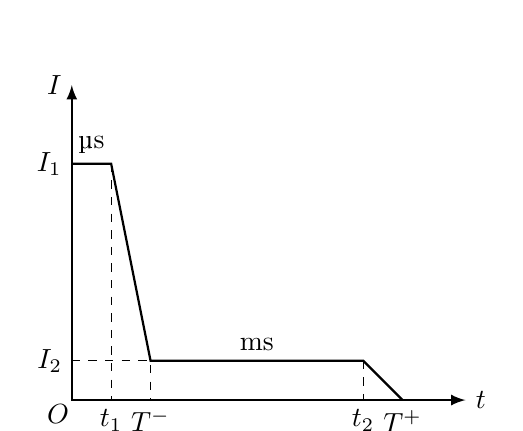
\begin{tikzpicture}
		\coor 54tI;
		\draw[thick](0, 3)node[left]{$I_1$}--(.5, 3)node[midway, above]{\si{\micro s}}--(1, .5)--(3.7, .5)node[midway, above]{ms}--(4.2, 0)node[below]{$T^+$};
		\draw[dashed](.5, 3)--(.5, 0)node[below]{$t_1$};
		\draw[dashed](0, .5)node[left]{$I_2$}--(1, .5)--(1, 0)node[below]{$T^-$};
		\draw[dashed](3.7, .5)--(3.7, 0)node[below]{$t_2$};
	\end{tikzpicture}
	\tikzchap 平板电离室的外回路电流
\end{center}
\begin{compactenum}
	\item $t_1\sim\si{\micro s}$开始有电子到达a极板,在$(0,t_1)$
	\[
		I_1=\frac{N_0e}d(u^-+u^+).
	\]
	\item $T^-$电子全部到达a极板;
	\item $t_2\sim\si{ms}$开始有正离子到达b极板,在$(T^-,t_2)$
	\[
		I_2=\frac{N_0e}du^+.
	\]
	\item $T^+$正离子全部到达b极板。
\end{compactenum}
随着载流子产生位置的变化,$t_1,t_2$也会相应变化。
\subparagraph{$R_L\neq 0$}
测量装置有输入阻抗,输出电压信号。
%脉冲电离室的
总电流信号
\[
	I_0=\frac V{R_0}+(C_a+C_1)\dv Vt=\frac e{V_0-V}\fkh{\sum_{j=1}^{N^+}\bm E\cdot\bm u^+-\sum_{k=1}^{N^-}\bm E\cdot\bm u^-}.
\]
由于$V\ll V_0$,可把电离室看成理想的内阻无限大的电流源。

把电离室看成理想电流源$I_0$和$C_1$并联等效。
\begin{center}
	\begin{tikzpicture}[circuit ee IEC]
		\foreach \contact/\x in {1/1.5, 2/3, 3/4.5, 4/6, 5/7.5} {
			\node [contact] (up \contact) at (\x, 2) {};
			\node [contact] (dn \contact) at (\x, 0) {};
		}
		\draw (0, 0) to [current source={direction info={}, info={$I_0$}}] (0, 2) to (9, 2);
		\draw (9, 0) to (0, 0) to [ground={at end}] (0, -.5);
		\draw (dn 1) to [capacitor={info={$C_1$}}] (up 1);
		\draw (dn 2) to [resistor={info={$R_L$}}] (up 2);
		\draw (dn 3) to [capacitor={info={$C'$}}] (up 3);
		\draw (dn 4) to [resistor={info={$R_i$}}] (up 4);
		\draw (dn 5) to [capacitor={info={$C_i$}}] (up 5);
		\draw[latex-latex](9, 0)--(9, 2)node[midway, fill=white]{$V$};
		\draw[dashed](-.8, -.2)rectangle(1.9, 2.2);
		\draw[dashed](2.1, -.2)rectangle(4.9, 2.2);
		\draw[dashed](5.1, -.2)rectangle(7.9, 2.2);
	\end{tikzpicture}
	\\
	$\Downarrow$
	\\[3ex]
	\begin{tikzpicture}[circuit ee IEC]
		\foreach \contact/\x in {1/1.5, 2/3} {
			\node [contact] (up \contact) at (\x, 2) {};
			\node [contact] (dn \contact) at (\x, 0) {};
		}
		\draw (0, 0) to [current source={direction info={}, info={$I_0$}}] (0, 2) to (4.5, 2);
		\draw (4.5, 0) to (0, 0) to [ground={at end}] (0, -.5);
		\draw (dn 1) to [capacitor={info={$C_0$}}] (up 1);
		\draw (dn 2) to [resistor={info={$R_0$}}] (up 2);
		\draw[latex-latex](4.5, 0)--(4.5, 2)node[midway, fill=white]{$V$};
	\end{tikzpicture}
	\tikzchap 电离室等效电路图
\end{center}
%电流,是载流子流动的产物。其大小由(1)载流子的数量,(2)载流子单位时间扫过的电位差占极板间压差的份额决定。
%这个电流被分享了,分享者至少包括:负载电阻、测量仪器的输入电阻。
%电流流过电阻必然有压降,因此探测器极板的压差自然也会改变,这进而使得与电阻并联的极板电容、分布电容、仪器输入电容的电压也发生变化、有了充放电,因此,这些电容也就要分享电流。
%所以,整个过程就是电场驱动一定数量的载流子在极板间运动,在外电路形成了感应电流,后者流经电阻和电容后形成了电压信号。
%这个道理对于后面的闪烁探测器、半导体探测器同样适用。
\paragraph{脉冲电离室的输出电压信号}
我们虽然写出了电流的公式,也理解了它的物理图像,但并不便于直接观察它,通常,我们分析的是电压信号!

解微分方程
\[
	I_0=\frac V{R_0}+C_0\dv Vt,\thus V(t)=\frac{\e{-t/R_0C_0}}{C_0}\int_0^tI_0(\tau)\e{\tau/R_0C_0}\d\tau.
\]
定义冲击响应函数
\[
	h(t):=\frac1{C_0}\e{-t/R_0C_0},\enspace t>0.
\]
方程的解可以写成卷积的形式
\[
	V(t)=I(t)\ast h(t).
\]
\begin{definition}{弹道亏损}{ballistic deficit}
	由于在给电容充电的同时,电容就已经开始通过电阻放电,导致电容上的最大电压$V\maxi<Q/C$的现象。($Q$表示电流面积)
\end{definition}
只有在$R_0C_0\to\infty$或电流$I(t)=\delta(t)$时,才没有弹道亏损。
但这两种情况都过于理想,因此弹道亏损总是存在的!

电流持续时间越长,弹道亏损程度越严重。%因此,电流的形状会影响弹道亏损的程度。

若电流的形状是确定的,则弹道亏损的程度就是确定的,有关系$Q\propto V$,可通过$V$来分析$Q$进而分析$E\dep$。
为保证$Q\propto V$,可令
\[
	R_0C_0\gg~\text{电流持续时间},
\]
此时弹道亏损可以忽略,对应离子脉冲电离室。
\subparagraph{离子脉冲电离室}
当$R_0C_0\gg T^+$时,全部电子和正离子对输出信号都有贡献,此时为离子脉冲电离室状态。
\begin{center}
	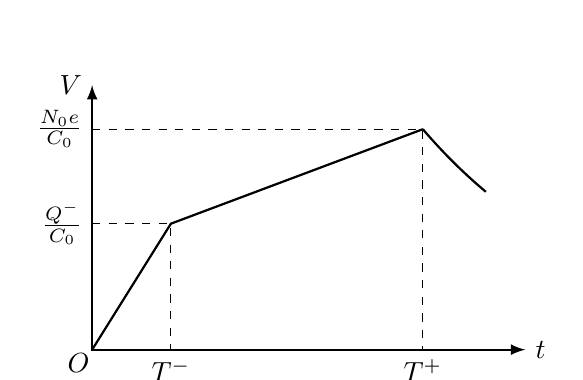
\begin{tikzpicture}[yscale=.8]
		\coor {5.5}{4.2}tV;
		\draw[thick](0, 0)--(1, 2)--(4.2, 3.5);
		\draw[thick, domain=4.2:5]plot(\x, {3.5^((7.2-\x)/3)});
		\draw[dashed](0, 2)node[left]{$\frac{Q^-}{C_0}$}--(1, 2)--(1, 0)node[below]{$T^-$};
		\draw[dashed](0, 3.5)node[left]{$\frac{N_0e}{C_0}$}--(4.2, 3.5)--(4.2, 0)node[below]{$T^+$};
	\end{tikzpicture}
	\tikzchap 离子脉冲电离室的电压信号
\end{center}
$(0,T^-)$离子电流+电子电流,$(T^-,T^+)$离子电流,$T^+$之后电容放电。在$t=T^+$时,电压信号的幅度最大,且
\begin{align}
	h:=V(T^+)=\frac{N_0e}{C_0}=\frac{e}{C_0}\frac{E\dep}W\propto E\dep.
\end{align}
因此可以测量射线的能量。

为了获得尽可能大的幅度,以抵抗后续电路的噪声,必须设法降低$C_0=C_1+C'+C_i$。

但由于要求$R_0C_0\gg T^+\sim\si{ms}$会带来问题:分辨时间大,限制了入射粒子的强度,否则会堆积;要求放大器电路频带非常宽,噪声大而非实用。
\subparagraph{电子脉冲电离室}
当$T^+\gg R_0C_0\gg T^-$时,正离子漂移的贡献可以忽略,仅有电子的贡献,此时为电子脉冲工作状态。
\begin{center}
	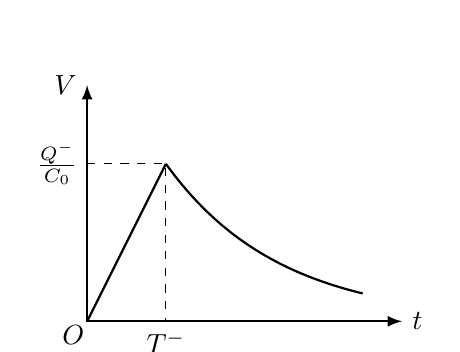
\begin{tikzpicture}
		\coor 43tV;
		\draw[thick](0, 0)--(1, 2);
		\draw[thick, domain=1:3.5]plot(\x, {2^(2-\x)});
		\draw[dashed](0, 2)node[left]{$\frac{Q^-}{C_0}$}--(1, 2)--(1, 0)node[below]{$T^-$};
	\end{tikzpicture}
	\tikzchap 电子脉冲电离室的电压信号
\end{center}
输出电压脉冲幅度
\[
	h=V(T^-)=\frac{Q^-}{C_0}\not\propto E\dep.
\]
与初始电离位置有关($Q^-$),不能用来测量射线能量$E\dep$。

由于$R_0C_0\ll T^+\sim\si{ms}$,因此可以大大降低脉冲宽度,获得小的分辨时间。另外,减小了频带的宽度,后续电路可以较好的抑制噪声。
\subsubsection{圆柱形电子脉冲电离室和屏栅电离室}
\paragraph{圆柱形电子脉冲电离室}
利用圆柱形电场的特点来减少$Q^-$对入射粒子位置的依赖,达到利用\textit{电子脉冲}来测量能量的目的。

圆柱形电场距中心位置为$r$的场强
\[
	E=\frac1r\cdot\frac{V_0}{\ln(b/a)}.
\]
电离会更多地发生在电位变化趋势缓慢的大半径处,将中央作为阳极,则大部分电子在漂向阳极时扫过的电荷量接近1个$e$。
\paragraph{屏栅电离室}
正极A、负极B、栅极G\footnote{屏蔽作用,使b区的电子离子不会在阳极A上产生感应电荷。}、电源和负载电阻。
\begin{center}
	\begin{tikzpicture}[circuit ee IEC]
		\draw [thick] (-4, 2.5) node [left] {Anode (A)} -- (-2, 2.5);
		\draw [thick] (-4, .5) node [left] {Cathode (B)} -- (-2, .5);
		\draw [dashed] (-4, 1.7) node [left] {Grid (G)} -- (-2, 1.7) node [above left] {a} node [below left] {b};
		\draw (-2, 1.7) -- (0, 1.7);
		\draw (-3, .5) to (-3, 0) to (0, 0) to [ground={at end}] (0, -.5);
		\draw (-3, 2.5) to (-3, 3) to [resistor={info={$R_L$}}] (0, 3) to [battery] (0, 1.7) node [contact] {} to [battery] (0, 0) node [contact] {};
		\draw [red] (-3.5, 1.5) -- (-2.5, .5) node [midway, above] {$R$};
	\end{tikzpicture}
	\tikzchap 屏栅电离室结构
\end{center}
结构要求:入射粒子将全部能量损失在b区。

入射粒子在b区产生电子离子对,电子在a区漂移时,在阳极A上形成感应电荷。
\subsubsection{脉冲电离室输出信号的测量}
\paragraph{入射带电粒子的数量}
测量输出脉冲数。
\paragraph{入射带电粒子的能量}
测量输出电压信号的幅度。
\paragraph{确定入射粒子间的时间关系}
测量输出电压信号的时间。
\subsubsection{脉冲电离室的性能}
脉冲电离室常用来测量带电粒子的能量。单能带电粒子若将全部能量都损耗在灵敏体积内,则输出电压脉冲的幅度反映了单个入射带电粒子能量的大小。
\paragraph{能量分辨率}
电离过程中的多次碰撞之间并非完全独立,离子对数目$N$服从Fano分布,当$N$很大时近似服从Gauss分布,由于
\[
	h=\frac{Ne}{C_0},
\]
电离室输出脉冲幅度$h$同样服从Gauss分布,故其半峰全宽(full width at half maxima, FWHM)
\[
	\FWHM=2\sqrt{2\ln2}\sigma_h\doteq 2.355\sigma_h.
\]

能量分辨率定义为FWHM比上均值$\avg h$
\[
	\eta:=\frac{\FWHM}{\avg h}=2.355\nu_h.
\]
又
\[
	\avg h=\frac e{C_0}\avg N,\quad\sigma_h=\frac e{C_0}\sigma_N=\frac e{C_0}\sqrt{F\avg N}.
\]
故能量分辨率为
\begin{align}
	\eta=2.355\sqrt{\frac{F}{\avg N}}=2.355\sqrt{\frac{FW_0}{E_0}}.
\end{align}
能量分辨率决定了谱仪所能达到的理论极限值,反映了谱仪对不同入射粒子能量的分辨能力。能量分辨率越好,可区分的能量差别也越小,是谱仪的主要指标之一。半导体探测器常用半宽度FWHM表征能量分辨特性
\[
	\FWHM=\eta E=2.355\sqrt{FWE}.
\]

能量分辨率的影响因素包括:统计涨落(statistical)、测量工作中条件的不稳定(drift)、探测器或电子学的随机噪声(noise)。
\[
	\FWHM^2=\FWHM_{\mathrm{stat}}^2+\FWHM_{\mathrm{drift}}^2+\FWHM_{\mathrm{noise}}^2.
\]
考虑drift因素。对于电离室谱仪,放大器输出的脉冲幅度为
\[
	h_A=A\frac{Ne}{C_0},
\]
$A$为放大倍数,故$\nu_{h_A}^2=\nu_N^2+\nu_A^2$

考虑noise因素,放大器噪声对输出幅度涨落的影响是叠加关系
\[
	h=h_1+h_2
\]
噪声的均值$\avg h_2=0$,定义信噪比$J$
\[
	J:=\frac{\avg h_1}{\sigma_{h_2}},
\]
电离室谱仪放大器输出信号的相对均方涨落$\nu_h^2$和能量分辨率$\eta$分别为
\[
	\nu_h^2=\frac F{\avg N}+\nu_A^2+\frac1{J^2},\quad \eta=2.355\sqrt{\frac F{\avg N}+\nu_A^2+\frac1{J^2}}.
\]
\paragraph{饱和特性曲线}
脉冲幅度$h$与电离室工作电压$V_0$的关系曲线。
\begin{center}
	\begin{tikzpicture}
		\coor64{V_0}h;
		\draw[thick](2, 2)parabola(0, 0);
		\draw[thick](2, 2)--(4, 2.1);
		\draw[thick](4, 2.1)parabola(5, 3)node[above]{正比区};
		\draw[dashed](0, 2)--(2, 2);
		\draw[dashed](0, 1.8)node[left]{90\%}--(1.37, 1.8)--(1.37, 0)node[below]{$V_1$};
		\draw[dashed](4, 2.1)--(4, 0)node[below]{$V_2$};
		\draw[dashed](2.25, 2)--(2.25, 0)node[below]{$V_{\mathrm{work}}$};
		\node[above right]at(0, 3){复合区};
		\node[above]at(2.75, 3){饱和区};
	\end{tikzpicture}
	\tikzchap 饱和特性曲线
\end{center}
对于脉冲探测器而言,希望工作在饱和区。
在达到饱和区脉冲幅度90\% 时对应饱和电压$V_1$,正比区前是放电电压$V_2$,在二者三等分点处是饱和区的工作电压$V_{\mathrm{work}}$。

饱和区并不是水平的,虽然射线的能量沉积并没有变,但提高电压会使灵敏体积变大,复合和扩散被进一步抑制,脉冲幅度会有微小增大。
\paragraph{坪特性曲线}
电离室的计数率$n$与工作电压$V_0$的关系曲线。
\begin{center}
	\begin{tikzpicture}
		\coor64hn;
		\draw[thick, domain=0:1.5]plot(\x, {3*exp(-4*\x*\x)});
		\node[right]at(0, 3){电子学噪声};
		\draw[dashed, domain=.25:1.75]plot(\x, {2*exp(-16*(\x-1)*(\x-1))});
		\node[below]at(1, 0){复合区};
		\draw[thick, domain=-1:1, shift={(3.6, 0)}]plot(\x, {1.2*exp(-6*\x*\x)});
		\draw[thick, domain=-1:1, shift={(4, 0)}]plot(\x, {exp(-4*\x*\x)});
		\draw[thick, domain=-1:1, shift={(4.4, 0)}]plot(\x, {.8*exp(-3*\x*\x)});
		\draw[dashed](3.6, 0)node[below]{$h_1$}--(3.6, 1.5);
		\draw[dashed](4, 0)node[below]{$h_2$}--(4, 1.5);
		\draw[dashed](4.4, 0)node[below]{$h_3$}--(4.4, 1.5);
		\node at(3, -1){(a)};
	\end{tikzpicture}
	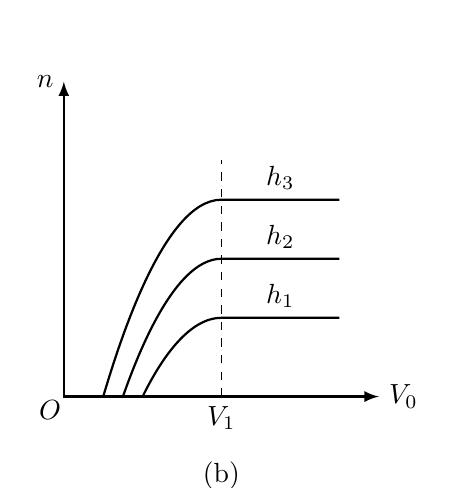
\begin{tikzpicture}
		\coor 44{V_0}n;
		\draw[dashed](2, 0)node[below]{$V_1$}--(2, 3);
		\draw[thick](3.5, 1)--(2, 1)node[midway, above]{$h_1$}parabola(1, 0);
		\draw[thick](3.5, 1.75)--(2, 1.75)node[midway, above]{$h_2$}parabola(.75, 0);
		\draw[thick](3.5, 2.5)--(2, 2.5)node[midway, above]{$h_3$}parabola(.5, 0);
		\node at(2, -1){(b)};
	\end{tikzpicture}
	\tikzchap (a) $n\vs h$曲线图;(b)坪特性曲线
\end{center}
入射粒子束流强度和入射粒子的能量保持不变,当输出脉冲幅度饱和后,计数率不再随工作电压变化;甄别阈$h_\thres$改变时,坪曲线也会改变。
\paragraph{探测效率}
绝对探测效率(absolute detection efficiency)
\[
	\varepsilon_{\mathrm{abs}}:=\frac{\text{脉冲数}}{\text{放射源放出粒子数}}.
\]
本征探测效率(intrinsic detection efficiency)
\[
	\varepsilon_{\mathrm{int}}:=\frac{\text{脉冲数}}{\text{射入灵敏体积的粒子数}}.
\]

带电粒子可能在灵敏体积内损失的能量较少,且电离过程是涨落的,信号脉冲幅度$<$甄别阈时,不能被记录。故带电射线$\varepsilon_{\mathrm{int}}\leqslant 100\%$

对中性射线,首先取决于与介质作用%产生次级带电粒子的
概率$\varepsilon=1-\e{-N\sigma D}<100\%$,然后次级带电粒子能否进入灵敏体积并沉积足够多能量。
\paragraph{时间特性}
分辨时间(死时间):能分辨开两个相继入射粒子间的最小时间间隔,由输出回路参数和放大器的时间常数决定。

时滞:入射粒子的入射时刻与输出脉冲产生的时间差。

时间分辨本领:由探测器输出脉冲来确定入射粒子入射时刻的精度。
\subsection{累计电离室}
入射粒子的强度$n$很大时,各个脉冲之间会发生叠加,探测器将无法再工作于脉冲模式,电离室的输出信号反映的是大量入射粒子的平均电离效应,其工作在累计或电流工作状态,此时电离室称作累计电离室或电流电离室。

%当$n$足够大,以至于在$R_0C_0$时间内的入射粒子数$\gg 1$,此时会形成直流电压信号,电流还是脉冲的;当$n$强大到在离子收集时间$T^+$内就有大量粒子入射,即使$R_0C_0=0$,$I_0(t)$也反映了大量粒子的平均电离效应,会形成直流电流信号。

假设:
\begin{compactenum}
	\item 单位时间内射入灵敏体积带电粒子数目的平均值$\avg n$不变;
	\item 带电粒子在灵敏体积内产生的离子对数目的平均值$\avg N$不变;
	\item 每个离子对产生后将立即使探测器产生一输出信号$S=f(t)$
\end{compactenum}
在时间间隔$\D\tau$内入射粒子产生的电子离子对数目$\D M=n\D\tau N$,推导得输出信号$S_t$的平均值和相对均方涨落为
\begin{align*}
	\avg S_t&=\avg n\avg N\int\zti f(\tau)\d\tau,\\
	\nu_{S_t}^2&=\frac1{\avg n}\kh{1+\frac F{\avg N}}\dvd{\int\zti f^2(\tau)\d\tau}{\kh{\int\zti f(\tau)\d\tau}^2}.
\end{align*}
可以看出,相对均方涨落$\nu_{S_t}^2$主要决定于入射粒子数$\D n$的涨落,离子对数$N$的涨落影响很小。
\paragraph{电流信号}用宽度为$T$的矩形脉冲近似代表一对离子所产生的电流信号
\[
	f(t)=\begin{cases}
		\frac eT,&t<T\\
		0,&t>T
	\end{cases}
\]
则电流信号的平均值和相对涨落为
\begin{align}
	\avg I&=\avg n\avg Ne,\\
	\nu_I^2&=\frac1{\avg n}\kh{1+\frac F{\avg N}}\frac1T\doteq\frac1{\avg nT}.
\end{align}
\paragraph{电压信号}
当$R_L\neq 0$时,在输出端输出一直流电压信号,一个离子对漂移在输出回路所产生的电压信号近似为一指数衰减信号:
\[
	f(t)=\frac e{C_0}\e{-t/R_0C_0}.
\]
则电压信号的平均值和相对涨落为
\begin{align}
	\avg V&=\avg n\avg NeR_0=\avg IR_0,\\
	\nu_V^2&=\frac1{\avg n}\kh{1+\frac F{\avg N}}\frac1{2R_0C_0}\doteq\frac1{2\avg nR_0C_0}.
\end{align}
要求输出电流或电压信号的相对均方涨落$\ll 1$,则
\begin{compactenum}
	\item 
	当入射粒子平均时间间隔$\ll$输出回路的时间常数:
	\[
		\frac1{2\avg n}\ll R_0C_0
	\]
	时,可视为直流电压信号;
	\item 
	当入射粒子平均时间间隔$\ll$电流脉冲宽度:
	\[
		\frac1{\avg n}\ll T
	\]
	时,可视为直流电流信号。
\end{compactenum}
\paragraph{小结}
\begin{compactenum}
	\item 脉冲电离室与累计电离室仅是电离室的两种工作状态;电离室结构并无本质差别。
	\item 入射粒子流的强度$n$及输出回路的时间常数$R_0C_0$、电流持续时间$T$决定了它工作在什么状态。
\end{compactenum}
\paragraph{累计电离室的主要性能}
饱和特性:同脉冲,工作于饱和区。

灵敏度($\si{A/cm^2.s}$)
\[
	\eta:=\frac{\text{输出电流(电压)幅度}}{\text{入射粒子流的强度}}.
\]
影响因素:电离室的结构、气体压力和组分、入射粒子的类型和能量等。

线性范围:输出信号幅度与入射粒子流强度保持线性关系的辐射强度范围。对应饱和区范围。当入射粒子流强度增大时,饱和电压将提高,会超过工作电压。

响应时间:入射粒子流强度发生变化时,输出信号的变化规律。电流主要由离子收集时间$T^+$决定,电压主要由时间常数$R_0C_0$决定。

能量响应:灵敏度随入射粒子能量而变化的关系。一般情况下,希望无能量响应。
\paragraph{累计电离室的应用}
累计电离室的应用比脉冲电离室更为广泛,特别是充入高压工作气体的
累计电离室,灵敏度高、性能稳定可靠、工作寿命长。

由于具有十分良好的承受恶劣工作环境影响的能力,所以在工业上可应
用于核辐射密度计、厚度计、料位计、水分计、核子秤等。
累计电离室还可应用于剂量测量、反应堆监测等方面。

\subsection{正比计数器}
脉冲电离室测量低能粒子(如$<\SI{100}{keV}$的X射线)时,放大器噪声使信噪比很小,测量难于进行。正比计数器能在探测器内部对电离信号进行放大,提高信噪比,就可以对低能粒子进行测量了。

正比计数器是一种非自持放电的气体电离探测器。利用碰撞电离将入射粒子直接产生的电离效应进行放大,使输出信号幅度比脉冲电离室显著增大。

要求:放大、均匀(位置一致)、线性(能量一致)。
\subsubsection{正比计数器的工作原理}
\paragraph{正比计数器的结构特点}
利用圆柱形电场的特点:\textit{在中央丝极附近会产生小范围的强电场区域}。
%强电场,以满足实现碰撞电离的要求()。
%一般采用非均匀电场实现,以圆柱型为主。

正比计数器的起始电压(阈压) $V_{\mathrm T}$,
\[
	V_{\mathrm T}=a\ln(b/a)E_{\mathrm T}.
\]
若工作电压$V_0<V_\mathrm T$,正比计数器仍是电离室;
$V_0>V_\mathrm T$时处于正比区,仅在$a\vs r_0$间发生碰撞电离。
\begin{example}{}{}
	$\SI{1}{atm}$下,电子在气体中的自由程$\sim\SIrange{e-4}{e-3}{cm}$,气体的电离电位$\sim\SI{20}{eV}$,电离所需的相应场强$E_\mathrm T=\SI{e4}{V/m}$。

	$a=\SI{80}{\micro m},b=\SI{1}{cm},V_0=\SI{4000}{V}$,计算得
	\[
		V_\mathrm T=\SI{386}{V},\quad r_0=\SI{410}{\micro m}.
	\]
	%碰撞电离
	电子漂移过的电位差
	\[
		V_\elc<\frac{\ln(r_0/a)}{\ln(b/a)}V_0=0.3384V_0,
	\]
	%碰撞电离
	离子漂移过的电位差
	\[
		V_\i>\frac{\ln(b/r_0)}{\ln(b/a)}V_0=0.6616V_0.
	\]
	故正比计数器输出电荷信号\textit{主要由正离子漂移贡献}。
\end{example}
$r_0$与$a$是同一数量级,故%入射粒子在$r_0$内产生初始电离的可能性很小,
$<r_0$处的初始电离很少。不同位置的初始电离都经受同样的气体放大过程。%故所有同一个气体放大倍数

正比计数器虽然是以离子电流为主,但它的离子电流是确定的、有快的成分,因此不必用大的$R_0C_0$
\paragraph{碰撞电离与气体放大}
电子到达距丝极一定距离$r_0$之后,通过碰撞电离过程,电子的数目不断增殖,这个过程称为气体放大过程,又称电子雪崩(electron avalanche)。定义气体放大倍数
\begin{align}
	A:=\frac{n(a)}{n(r_0)}.
\end{align}
放大倍数与Townsend系数
\[
	\alpha:=\frac1n\dv nx.
\]
有关,$\alpha$是气体类型和约化场强的函数。
\newpage
均匀电场$A=\e{\alpha\D x}$与初始位置有关,而圆柱形电场
\[
	A=\exp\biggkh{-\int_{r_0}^a\alpha\d r}.
\]
与初始电离位置无关。

$\alpha=N\sigma$,碰撞电离截面$\sigma$正比于电子的动能,故当$V_0\gg V_\mathrm T$时,
\[
	\ln A\propto V_0
\]
\paragraph{气体放大过程中的光子作用}
在电子与气体分子的碰撞中,不仅能产生碰撞电离,同时也能产生碰撞激发,退激发出的紫外光子能量一般大于阴极材料的表面逸出功,可在阴极(或其它气体分子)打出次电子,次电子在电场加速下也可发生碰撞电离,称为\textbf{光子反馈}。

定义每个到达阳极的电子通过光子反馈又在阴极打出一个次电子的概率为光子反馈概率$\gamma$,光子反馈使得总放大倍数增加为
\[
	A\tot=A+\gamma A^2+\gamma^2A^3+\cdots=\frac A{1-\gamma A}.
\]

\begin{compactitem}
	\item 光子反馈时间(\si{ns}) $\ll$电子漂移时间(\si{\micro s}),对信号形成而言可认为是同时事件。
	\item 加入少量多原子分子气体M (CO$_2$, CH$_4$)的作用:M可以强烈吸收紫外光子而处于激发态M$^*$,M$^\ast$不再发出光子而是分解为几个小分子(超前离解),这样可以阻止紫外光子打到阴极而减小光子反馈,使$\ln A\propto V_0$曲线的变化平缓,使发生自持放电的电压更高,以获得更大的正比工作区间。
\end{compactitem}
\paragraph{气体放大过程中正离子的作用}
空间电荷效应(space charge effect):在电子漂移、碰撞电离等过程中,漂移速度慢的正离子可认为基本没动,在阳极丝附近形成空
间电荷,使阳极丝附近的电场强度变弱,影响电子雪崩过程。%影响空间电场、进而影响倍增过程。

离子反馈:正离子漂移到达阴极,在与阴极表面的感应电荷中和时有一定概率产生次电子,发生新的电子雪崩过程。可以通过加入少量多原子分子气体阻断。

正比计数器雪崩不是很强烈,一个地方发生的雪崩并不妨碍其他地方能不能够发生雪崩。
\subsubsection{正比计数器的输出信号}
\paragraph{离子电流}假定:
\begin{compactenum}
	\item $A\gg 1$:忽略初始电离的载流子对输出信号的贡献。
	\item $r_0$很小:电子的阴极感应电荷很小→忽略电子对输出信号的贡献。
	\item 全部输出信号为雪崩后正离子由阳极表面向阴极漂移在外回路流过的感应电荷。
\end{compactenum}
则
\begin{gather*}
	I=A\frac{Ne}{V_0}\bm E\cdot\bm u^+,\\
	u^+=\mu^+\frac EP,\thus\dv rt=\frac{\mu^+}P\frac{V_0}{r\ln(b/a)}.
\end{gather*}
得到
\[
	I=\frac{ANe}{2\ln(b/a)}\frac1{t+\tau},\quad\tau:=\frac{a^2P\ln(b/a)}{2V_0\mu^+}=\SI{15.1}{ns}.
\]
故电流$I$随时间$t$下降地很快!
\begin{align}
	I\propto\frac1{t+\tau}.
\end{align}
离子电流虽然持续时间很长,但很早就扫过了大部分电荷

无论射线在哪里发生初始电离,正比计数器输出电流的形状总是确定的,则电压信号的弹道亏损程度总是确定的。
电流面积受两个因素影响:初始电离的载流子数目$N_0\propto E\dep$;倍增系数$A$反映雪崩的剧烈程度,对一个确定的探测器来说,$A$的期望值仅由工作电压$V_0$决定。
因此正比计数器输出电压信号的幅度$h\propto E\dep$,这是很重要的特点。
\paragraph{电压信号}
\[
	V_0=\frac{ANe}{2C_0\ln(b/a)}\e{-t/R_0C_0}\int_0^t\e{t'/R_0C_0}\frac{\d t'}{t'+\tau}.
\]
电压脉冲信号与粒子入射位置无关,$R_0C_0$的选取虽会影响电压幅度,但$h\propto N$仍成立。

由于离子电流在早期即\textit{扫过了大部分电荷},因此可以在不过分减小信号幅度的情况下,减小$R_0C_0$以实现高的计数率。
\subsubsection{正比计数器的性能}
\paragraph{输出脉冲幅度与能量分辨率}
输出脉冲幅度$h\sim ANe/C_0$是一个二级串级型随机变量,其相对涨落
\[
	\nu_h^2=\nu_N^2+\frac1{\avg N}\nu_M^2=\frac1{\avg N}\kh{F+\nu_M^2}.
\]
实验表明$\nu_M^2\doteq 0.68$,故能量分辨率
\begin{align}
	\eta=2.355\sqrt{\frac{F+0.68}{\avg N}}.
\end{align}
影响正比计数器能量分辨率的其它因素:阳极丝的均匀性、负电性气体的存在、末端效应和室壁效应、电子学系统的影响。
\[
	\nu_{h_A}^2=\frac F{\avg N}+\frac1{J^2}+\nu_A^2=\frac F{\avg N}+\frac{\nu_M^2}{\avg N}-\kh{\frac{C_0\sigma_{h_2}}{ANe}}^2+\nu_A^2.
\]
在满足信噪比的前提下,可用小的倍增系数,有利于:减少非线性、获得好能量分辨率。
\paragraph{探测效率和坪特性}
分立$\vs$连续,见讲义
\paragraph{分辨时间$\tau$和计数率修正}
分辨时间$\tau$:主要由输出脉冲的宽度决定。%脉冲越宽,死时间越大。在$\tau$内再产生的脉冲不会被记录,从而会造成计数的损失,为此必须考虑计数率的修正。

任何一个信号,只有当其前面$\tau$时间内无信号时,才能被计数。考虑平均计数率为$m$,则$\tau$内无信号的概率为$\e{-m\tau}$,因此,实际测量到的计数率$n=m\e{-m\tau}$,当$m\tau\ll 1$时,
\begin{align}
	n=m\e{-m\tau}\doteq m(1-m\tau),\thus m\doteq\frac n{1-n\tau}.
\end{align}
第二个射入探测器的射线能否被探测器响应要看探测器测量它的条件是否具备。就正比计数器来说,有气体可初始电离形成自由电子,有电场可雪崩,%只要不恰巧在上个射线正离子未漂走的雪崩处,
则第二个射线肯定是可以被探测器响应的。%同理,第三个、第四个……也是可以被响应的。

但是电路只有一个,这些被响应射线的输出信号可能就由于其间隔小于分辨时间而不得不叠加为一个电信号,这就是计数率损失的来源。
\paragraph{时滞与时间分辨本领}
时滞(\si{\micro s}):初始电子由产生处漂移到阳极附近所需的时间。

时间分辨本领(\si{\micro s}):正比计数器对时间的测量精度。由于初始电子产生位置的随机性,因此时滞也具有随机性,从而限制了时间分辨本领。
\subsubsection{正比计数器的应用}
能量测量——正比谱仪

正比计数器在强度测量方面的应用

单丝位置灵敏正比计数器

多丝正比室

GEM探测器
\subsection{G-M计数管}
G-M计数管是由Geiger和Müller于1928年发明的一种利用自持放电来进行射线探测的气体电离探测器,它也许是最著名的射线探测器。

G-M管的优点:制造简单、价格便宜、使用方便、灵敏度高、输出电荷量大($10^8e$);缺点:死时间长、仅能用于计数。
%✓
\subsubsection{非自熄G-M管的工作机制}
在正比计数器中,光子反馈和正离子反馈的作用极微弱,因此,经一次雪崩以后增殖过程即行终止,且雪崩只限于局部的区域,对一个初始电子仅展宽$\SI{200}{\micro m}$左右;但在G-M计数管中,光子反馈和离子反馈就成为重要的过程。

由于光子反馈过程的存在,气体放大倍数为
\[
	A\tot=\frac A{1-A\gamma},
\]
通常条件下光子反馈概率为$\gamma\sim 10^{-5}$,若$A\sim 10^5$,则$A\tot\to\infty$

G-M管的自持放电过程可以分解为下列环节:
\begin{compactenum}
	\item 初始电离及碰撞电离过程:电子加速发生碰撞电离形成电子潮(雪崩)。
	\item 放电传播:Ar$^*$放出的紫外光子打到阴极上并打出次电子(光子反馈)。
	
	一处点火,全丝放电:气体放电迅速遍及整个管子。
	
	电子很快被阳极收集,形成电子电流;正离子包围整个阳极丝,并逐步加厚形成正离子鞘。由于正离子鞘的形成,使阳极丝附近的电场减弱,使放电终止。
	\item 正离子鞘向阴极漂移,形成离子电流,是形成输出脉冲的主要贡献。
	\item $\sim\SI{100}{\micro s}$后正离子在阴极表面发生电荷中和,形成\textbf{离子反馈}:
	\[
		\nuc{Ar}^++\elc^-\to\nuc{Ar}^\ast\overset{\star}\semilongrightarrow\elc^-\overset{\text{加速}}\semilongrightarrow\nuc{Ar}^++\nuc{Ar}^\ast+\elc^-\overset{\text{加速}}\semilongrightarrow\cdots
	\]
	$\star$:Ar$^\ast$退激发射光子打到阴极或Ar$^\ast$直接到达阴极。

	它们发生在第一次正离子漂移快结束时;阴极产生的电子向阳极漂移又引起新的雪崩,形成第二个脉冲;如此周而复始,形成了自持放电,所以被称作非自熄G-M计数管。
\end{compactenum}
\paragraph{如何实现自熄?}雪崩的两个条件:电场和电子。

外因自熄(external quenching):改变工作高压(影响电场)。在脉冲产生后,降低工作高压,使倍增条件不具备,持续时间应该包括:
\begin{compactitem}
	\item 离子由正离子鞘漂移到阴极的时间:$\sim\SI{100}{\micro s}$
	\item 阴极产生的自由电子运动到阳极的时间:$\sim\si{\micro s}$
\end{compactitem}
可以在外电路选用大电阻($R\sim\SI{e8}{\ohm}$),$R_0C_0\sim\si{ms}$,满足自熄要求,但也需要$\sim\si{ms}$来使阳极恢复到正常工作状态,因此计数率低。

内因自熄(internal quenching):增加猝熄气体(影响电子),比如有机自熄G-M管、卤素自熄G-M管。
\subsubsectionstar{有机自熄管的工作机制}
有机自熄管是在工作气体中加入少量有机气体M (多原子分子气体,又称猝熄气体)具有自熄能力的G-M管。例如,90\% Ar + 10\% C$_2$H$_5$OH。

阻断光子反馈,阻断离子反馈……

工作电压较高、寿命较短。
\subsubsectionstar{卤素自熄管的工作机制}
Ne为主要工作气体,并在其中加入微量卤素气体(如1\% Br)

自动猝熄、较低阈压、寿命较长、放电区域较大、卤素为负电性气体(影响卤素计数管的特性,尤其是坪特性曲线。有机管的坪特性好些)
\subsubsection{自熄G-M管的输出信号}
自熄G-M计数管输出脉冲形状与正比计数管无明显区别。和正比计数器一样,输出脉冲由两个部分组成:
\begin{compactenum}
	\item 电子收集、正离子漂移初期的快上升部分
	\item 正离子漂移期间的缓慢上升部分
\end{compactenum}
\begin{center}
	\tablechap{正比计数器与G-M管比较}
	\begin{tabular}{ccc}
		\toprule
		&正比计数器&G-M管\\
		\midrule
		输出信号的幅度&$\propto E\dep$&与能量无关\\
		用途&测能谱、计数&只能用于计数\\
		\bottomrule
	\end{tabular}
\end{center}
\subsubsection{自熄G-M管的性能}
G-M管的性能由以下因素决定:计数管的阳极丝半径$a$、阴极半径$b$、工作气体的组成与压力。

主要性能包括:坪特性曲线、探测效率、时间特性
\paragraph{坪特性曲线}计数率与工作电压的关系……

坪斜的成因:随工作电压的增高,
\begin{compactenum}
	\item 正离子鞘电荷量增加,猝熄不完善的可能性增加
	\item 负电性气体的电子释放概率增加
	\item 灵敏体积增大
	\item 结构的尖端放电增加
\end{compactenum}
\paragraph{探测效率}
对用于带电粒子探测的钟罩型G-M管,只要入射粒子进入灵敏体
积,其探测效率可接近100\%。

对用于探测$\gamma$射线的圆柱型G-M管,仅当次电子进入灵敏体积才能引起计数,其探测效率仅$\sim 1\%$。
\paragraph{时间特性}
\begin{compactitem}
	\item \textbf{失效(死)时间}$t_\mathrm d\sim\SI{100}{\micro s}$:随正离子鞘向阴极漂移,使电场屏蔽逐渐减弱、电子又能在阳极附近发生雪崩的时间。
	\item \textbf{时滞}:在气体中生成第一个离子对的时间与第一个雪崩的时间存在延迟,且延迟时间与第一个离子对生成的位置有关。其差别$\SIrange{0.1}{0.4}{\micro s}$,会导致这一量级时间测量的不准确性。
	\item \textbf{时间分辨本领}$\sim\si{\micro s}$,采取特殊措施后可$\sim\SI{0.1}{\micro s}$。
	\item \textbf{复原时间}$t_\mathrm e\sim\SI{100}{\micro s}$:从上一个事件开始,输出脉冲幅度恢复到正常的时间。
	\item \textbf{分辨时间}$t_\mathrm f\sim\SI{100}{\micro s}$:从0到下一个脉冲超过甄别阈的时间,与甄别阈的大小有关。\footnote{一般死时间同分辨时间,但G-M管的死时间特指失效时间,是分辨时间的一部分。}
\end{compactitem}
G-M管中,由于正离子鞘覆盖了整个阳极丝,在第一个粒子引起的死时间内,不能产生新的雪崩,死时间因此不再扩展。\footnote{G-M管大概是死时间唯一不可扩展的探测器类型了,本课程的其它探测器(电离室、正比计数器、闪烁探测器、半导体)的死时间都是可扩展的,其共同的机制就是:\textit{一个射线的入射不会使探测器失能、从而导致无法响应下一个时间上邻近的入射射线。}}

真事件的计数率为$m$,探测器死时间为$\tau$,记录到的计数率为$n$,则有
\begin{align}
	\frac1m=\frac1n-\tau.
\end{align}
\paragraph{寿命}计数寿命:有机管$\sim 10^8$次计数,卤素管$\sim 10^9$次计数;

搁置寿命:卤素管中的卤素较活泼,寿命较短。有机管可保证长达几年的搁置寿命。
\paragraph{输出回路对计数管特性的影响}
在G-M管中,尤其是对卤素管,其放电区域较大,电子漂移对输出信号的贡献比正比计数器要大,对放电终止有影响。

尽可能减小分布电容有利于提高输出脉冲幅度,对放电终止也起到积极作用。
\subsubsectionstar{自熄G-M管的结构与典型应用}
G-M管主要有:
\begin{compactenum}
	\item 圆柱型:主要用于$\gamma$射线测量
	\item 钟罩型:由于有入射窗,主要用于$\alpha,\beta$射线的测量
\end{compactenum}
\newpage
\paragraph{气体探测器的问题?}气体探测器的能量分辨率
\[
	\eta=2.355\nu_h=2.355\sqrt{\frac{F+0.68}{\avg N}}
\]
是不错的,对重带电粒子和低能光子的测量是出色的。

但它不能测量高能光子,原因:
\begin{compactenum}
	\item 与MeV光子的反应概率$1-\e{-N\sigma D}$
	\item 对MeV电子能量的沉积能力
\end{compactenum}
我们下面讨论闪烁体探测器。
\clearpage
\section{闪烁探测器}
闪烁探测器(scintillation detectors)是利用辐射在某些物质中产生的闪光来探测电离辐射的探测器。
闪烁探测器的优点:
\begin{compactenum}
	\item 密度、体积大,对中性射线($\gamma,\nton$)的探测效率高,易于沉积能量,因此能够测量能谱。
	\item 时间特性好,有的探测器(如塑料闪烁体、BaF$_2$)可实现ns的时间分辨能力。
\end{compactenum}
\subsection{闪烁探测器的基本原理}
闪烁探测器是利用辐射在闪烁体内闪光来探测电离辐射的探测器。
由
闪烁体、
光电倍增管(photomultiplier tube, PMT)、
高压电源、
低压电源、
分压器、
前置放大器
构成。
其工作过程为:
\begin{compactenum}
	\item 射线沉积能量,电离能损产生带电粒子
	%电离能损:γ射线制造三种次级电子,中子核反应后的带电粒子,或者带电粒子直接入射。
	\item 带电粒子使闪烁体电离或激发,退激后发出大量荧光光子(可见光);
	\item 荧光光子被PMT的光阴极转换为光电子,并被第一打拿极收集;
	\item 电子在PMT的打拿极间运动并倍增(\numrange{e7}{e10});
	\item 流经外回路
	%决定工作状态:电流脉冲型、电压脉冲型?
\end{compactenum}
\subsubsection{闪烁体}
高探测效率(高$Z$、高密度、大尺寸)、
高发光效率、
能量线性好、
自吸收小、
发光时间短、
可加工性好、
易于耦合(合适的折射率)
\paragraph{闪烁体的分类}
\begin{compactitem}
	\item 无机闪烁体:探测效率高、光输出产额高、线性好;但发光时间较长
	\begin{compactitem}
		\item 纯晶体:BGO, BaF$_2$
		\item 无机盐晶体:NaI(Tl), ZnS(Ag)
		\item 玻璃体:Li$_2$O$·$2SiO$_2$(Ce)
	\end{compactitem}
	\item 有机闪烁体:发光时间短;但光输出产额低、光电截面低
	\begin{compactitem}
		\item 有机晶体:蒽,萘,芪
		\item 有机液体闪烁体
		\item 塑料闪烁体
	\end{compactitem}
	\item 气体闪烁体:Ar, Xe
\end{compactitem}
\paragraph{无机闪烁体的发光机制}
以NaI(Tl), CsI(Tl),CsI(Na)等为最典型,又称卤素碱金属晶体(Alkali Halide Scintillator)。

入射带电粒子在闪烁体内电离,产生电子-空穴对或激子(exciton);
导带上电子和价带上空穴可以复合成激子,
激子吸收热运动能量也可变成电子-空穴。
退激可能发出光子,也可能使晶格振动而不发光。

纯离子晶体退激发出的光子容易被晶体自吸收,传输出的光子少;禁带宽度大,退激发光在紫外范围,光阴极不响应。

晶体掺杂$10^{-3}$量级的激活剂(activator),形成特殊晶格点,在禁带中形成局部能级。
电子-空穴迁移到杂质原子处,使杂质原子处于激发态,形成发光或复合中心(luminescence/recombination centers)。杂质原子退激:
\begin{compactitem}
	\item 荧光(fluorescence):1$\SIrange{10}{500}{ns}$。
	\item 磷光(phosphorescence):亚稳态,发光时间较长,是afterglow的主要部分。
	\item 猝灭(quenching):转换为晶格的热运动。
\end{compactitem}
\paragraph{有机闪烁体的发光机制}
有机闪烁体都是苯环化合物,分子之间仅有松散的范德瓦尔斯力。其激发与发光是由分子自身的激发和跃迁产生
的。荧光在ns级,磷光在ms级或更长。

发射、吸收光谱的峰值是分开的,因此有机闪烁体对其所发射的荧光是透明的。
在溶剂中加入高效闪烁物质,可提高闪烁效率,构成二元有机闪烁体。
发射谱的短波部分与吸收谱的长波部分有重叠,可在有的有机闪烁体中加入移波剂,以减少自吸收。
\subsubsection{闪烁体的物理特性}
\paragraph{发光光谱}
闪烁体发射光子数与光子波长(能量)的关系曲线,与闪烁体、激活剂(移波剂)、温度有关。
\paragraph{发光效率}
希望发光效率较高,且对不同能量保持常数。
\begin{compactenum}
	\item 光能产额(光输出,光产额)
	\[
		Y_{\mathrm{ph}}:=\frac{\avg n_{\mathrm{ph}}}{E\dep}.
	\]
	NaI(Tl)晶体$Y_{\mathrm{ph}}=\SI{4.3e4}{/MeV}$,每荧光光子$\SI{23}{eV}$。
	\item 闪烁效率(发光效率,能量转换效率)
	\[
		C_{\mathrm{np}}:=\frac{E_{\mathrm{ph}}}{E\dep}=\frac{h\avg\nu}{E\dep}.
	\]
	\item 相对闪烁效率(相对发光效率)
\end{compactenum}
\paragraph{闪烁发光时间}
由上升时间与衰减时间决定

可能有快、慢成分。
\paragraph{其它特性}
探测效率等
\subsubsection{光的收集与光导}
闪烁光的收集需要:
\begin{compactitem}
	\item 光学反射层:让光向光阴极的方向传播。
	反射方式
	\begin{compactitem}
		\item 镜面(specular)反射:铝箔、镀铝塑料薄膜
		\item 漫反射(diffuse):MgO、TiO$_2$、聚四氟乙烯塑料带等
	\end{compactitem}
	\item 光学耦合剂:让光可以射出闪烁体。
	
	光子由光密物质射向光疏物质时,存在发生全反射的临界角,在闪烁体与PMT间填充光学耦合剂,可以让更多角度的光射出闪烁体。
	\item 光导:连接闪烁体与光电转换器件。
	
	利用大折射系数材料的全反射。
\end{compactitem}
\subsection{光电倍增管}
\paragraph{光电倍增管的类型}略
\paragraph{光电倍增管的结构与工作原理}
光电倍增管结构:
\begin{compactenum}
	\item 光学窗:光阴极所附着的结构
	\item 光阴极(photocathode):通过光电效应将荧光光子转换为光电子。%所有光阴极都有截止波长,因此并非所有光子都会被转换为电子。
	\item 打拿极(dynode):电子倍增
	\item 阳极(anode):收集电子
\end{compactenum}

打拿极要求:
次级电子产额大;
热电子与光电子发射小;
大电流工作时性能稳定;
快速响应。

打拿极的次级电子产额$\delta$
\[
	\delta:=\frac{\text{发射的次级电子数}}{\text{入射的初级电子数}}.
\]

\paragraph{光电倍增管的供电回路}
\begin{compactenum}
	\item K-D$_1$电压较高(几倍于其它打拿极间的电压),可有效收集光电子,减少电子飞行时间的离散;
	\item 中间各打拿极均匀分压;
	\item 最后几个打拿极间高电压、大电流,需要电容稳压;
	\item 最后打拿极与阳极间电压较小。
\end{compactenum}
分压电路:提供静态工作点,直流电流应显著大于脉冲电流。

分压器所用电阻的温度系数应当小,稳定性高。
总功率不要太大,以免PMT因为温度升高而漂移

正高压供电方式阴极接地即可;但
需要隔直电容:
不适合于累计状态、
易受高压纹波的影响。

负高压供电方式无需隔直电容,适合高计数率、定时特性好、适合累计状态;但阴极处于高压,需防止与周围接地材料之间的高压漏电信号、场致发光(玻璃)。
\paragraph{光电倍增管的主要性能}
\begin{compactitem}
	\item 光阴极的光谱响应:光阴极发射光电子的几率与光子波长的关系,定义量子效率
	\begin{align}
		Q_\mathrm k(\lambda):=\frac{\text{发射电子数}}{\text{入射光子数}}.
	\end{align}
	NaI(Tl):若$Q=25$ - 30\%,则$\SIrange{100}{120}{eV/\text{光电子}}$
	\item 光阴极、阳极的光照灵敏度:
	\[
		S_\mathrm k=\frac{i_\mathrm k}F,\quad S_\mathrm a=\frac{i_\mathrm a}F.
	\]
	$i_\mathrm k,i_\mathrm a$是阴极电流和阳极电流(A),$F$是入射到光阴极的光通量(lm)
	\item 第一打拿极(D1)的电子收集系数
	\[
		g_\mathrm c:=\frac{\text{第一打拿极收集到的光电子数}}{\text{光阴极发出的光电子数}}.
	\]
	$g_\mathrm c$对PMT的幅度分辨率影响较大,在有聚焦极的光电倍增管中,$g_\mathrm c>95\%$
	\item 光电倍增管的电流放大倍数
	\[
		M=\frac{\text{阳极收集到的电子数}}{\text{第一打拿极收集到的光电子数}}=(g\delta)^n.
	\]
	$g$为电子传输效率,$\delta$为各级电子倍增系数,$n$为倍增级数。
\end{compactitem}
则%荧光光子数目$\avg n_{\mathrm{ph}}=E\dep Y_{\mathrm{ph}}$,
光电转换因子
\[
	\avg T:=F_{\mathrm{ph}}\avg Q_\mathrm kg_\mathrm c,
\]
$F_{\mathrm{ph}}$为光子传输系数,则D1光电子数$n_\elc=Tn_{\mathrm{ph}}$。

PMT输出脉冲中的电荷量
%Q=E\dep Y_{\mathrm{ph}}F_{\mathrm{ph}}\avg Q_\mathrm kg_\mathrm c\avg Me,
\begin{align}
	Q=\avg n_{\mathrm{ph}}\avg T\,\avg Me.
\end{align}
\begin{compactitem}
	\item PMT的时间特性:
	\begin{compactitem}
		\item 渡越时间$t_\elc\sim\SIrange{20}{80}{ns}$:从光电子离开光阴极算起各电子到达阳极的时间。影响时滞。
		\item 渡越时间离散$\D t_\elc\sim\si{ns}$:到达阳极的每个电子都经历了不同的倍增过程和飞行距离,导致了飞行时间的涨落。
		
		影响系统的时间分辨能力;对于有机闪烁体,也影响探测器的分辨时间。
	\end{compactitem}
\end{compactitem}
\subsection{闪烁探测器的输出信号}
\paragraph{闪烁探测器输出信号的物理过程}
倍增电子向后级漂移,
感应电流从外回路流过。
\paragraph{闪烁探测器的输出回路}
信号可从回路取,也可从前级打拿极(D$_{n-1}$)取信号。
\subsubsection{电流脉冲信号}
光电倍增管的单电子响应函数$p(t)$:
\begin{compactitem}
	\item 对于大部分无机闪烁体,$p(t)$可以近似看做一个延迟的$\delta$函数;
	\item 对于有机闪烁体,$p(t)$的展宽和发光时间相当,不能看做$\delta$函数。
\end{compactitem}
无机闪烁体,一次闪烁光引起的输出电流
\[
	I(t)=\frac{n_{\mathrm{ph}}TMe}{\tau_0}\e{-(t-t_\elc)/\tau_0},\quad t\geqslant t_\elc.
\]
$\tau_0\sim\SI{250}{ns}$为发光衰减时间。
\subsubsection{电压脉冲信号}
输出电压信号的一般形式
\[
	V(t)=\frac1{C_0}\e{-t/R_0C_0}\int_0^tI(\tau)\e{\tau/R_0C_0}\d\tau,
\]
代入上式得
\[
	V(t)=\frac Q{C_0}\frac{R_0C_0}{R_0C_0-\tau_0}\kh{\e{-t/R_0C_0}-\e{-t/\tau_0}},
\]
\begin{compactitem}
	\item $R_0C_0\gg\tau_0$,
	\begin{align*}
		V(t)&\doteq\frac Q{C_0}\kh{\e{-t/R_0C_0}-\e{-t/\tau_0}}\\
		&=\begin{cases}
			\frac Q{C_0}\kh{1-\e{-t/\tau_0}},&t\ll\tau_0\\
			\frac Q{C_0},&\tau_0\ll t\ll R_0C_0\\
			\frac Q{C_0}\e{-t/R_0C_0},&t>R_0C_0
		\end{cases}
	\end{align*}
	\item $R_0C_0\ll\tau_0$,
	\begin{align*}
		V(t)&\doteq\frac{R_0Q}{\tau_0}\kh{\e{-t/R_0C_0}-\e{-t/\tau_0}}\\
		&=\begin{cases}
			\frac{R_0Q}{\tau_0}\kh{1-\e{-t/R_0C_0}},&t\ll\tau_0\\
			\frac {R_0Q}{\tau_0},&R_0C_0\ll t\ll \tau_0\\
			\frac {R_0Q}{\tau_0}\e{-t/\tau_0},&t>\tau_0
		\end{cases}
	\end{align*}
	\item $R_0C_0=\tau_0$,
	\[
		V(t)=\frac{Q}{C_0}\frac{t}{R_0C_0}\e{-t/R_0C_0},
	\]
	
	\item $C_0$不变,随着$R_0$的增大,幅度、脉宽都增大;
	\item $R_0$不变,随着$C_0$的增大,幅度降低、脉宽增大。
\end{compactitem}

闪烁探测器电流信号的形状总是确定的\footnote{本课程仅二例是电流形状确定的:正比计数器、闪烁体探测器。},因此弹道亏损的程度是确定的。无论$R_0C_0$怎样改变,$V\maxi\propto Q\propto E\dep$的关系总存在,可以测量射线的沉积能量。

实际中常选取$R_0C_0=\tau_0$,幅度足够大,脉宽足够窄。同时,$C_0$应尽可能小,以获得大的脉冲幅度。
\paragraph{电压脉冲型 vs 电流脉冲型工作状态}
所谓电压型脉冲信号和电流型脉冲信号,说的都是电流信号流经外回路后的电压信号。$R_0C_0$和$\tau_0$之间的大小关系,决定了是哪种脉冲信号。
\begin{compactitem}
	\item 电压型脉冲信号($R_0C_0\gg\tau_0$)的重点在于(通过脉冲幅度)分析电流信号的面积,希望电压信号的幅度够大,能抵抗后续电路的噪声,获得好的能量分辨率。
	\item 电流型脉冲信号($R_0C_0\ll\tau_0$)的重点则在于如实地反映电流信号的形状。这在PSD(Pulse Shape Discrimination)技术识别粒子种类的应用中非常重要(例如$\nton/\gamma$识别)。
\end{compactitem}
\subsubsection{输出信号的涨落}
光电倍增管输出电荷数$n_a$是个串级型随机变量:
\begin{compactitem}
	\item 闪烁体发出的光子数$n_{\mathrm{ph}}$,近似服从Poisson分布;
	\item 光子能否转换为第一打拿极收集到的光电子,是Bernoulli事件,期望值为$T$;
	\item 第一打拿极收集到的光电子数$n_\elc$为泊松分布;
	\item PMT的电子倍增系数$M$。
	\[
		\avg M=\avg\delta_1\avg\delta^{n-1},\thus\nu_M^2=\frac1{\avg\delta_1}\cdot\frac{\avg\delta}{\avg\delta-1},
	\]
\end{compactitem}
由$\avg n_a=\avg n_{\mathrm{ph}}\avg T\,\avg M$,可得 
\begin{align}
	\nu_{n_a}^2=\frac1{\avg n_{\mathrm{ph}}\avg T}\biggkh{1+\frac1{\avg\delta_1}\cdot\frac{\avg\delta}{\avg\delta-1}},
\end{align}
第一打拿极的倍增系数$\delta_1$大些为好,比如负电子亲和(NEA)材料。
\subsection{闪烁探测器的主要性能}
\paragraph{$\gamma$闪烁谱仪的组成与工作原理}
探测次级电子能谱:光电效应、Compton效应、电子对效应。
\subsubsection[单能\textit{\textgamma}射线的次级电子能谱]{单能$\gamma$射线的次级电子能谱}
\begin{compactitem}
	\item 小尺寸闪烁体:仅吸收次级电子的能量
	\item 大尺寸闪烁体:吸收全部次级电子、次级电磁辐射能量
	\item 中等尺寸闪烁体(实际情况):吸收次级电子能量,以一定几率吸收次级电磁辐射能量。
\end{compactitem}
还要考虑“不速之客”:来自环境的“散射”。

\textbf{务必看讲义里的图}。
\subsubsection[\textit{\textgamma}射线的输出脉冲幅度谱]{$\gamma$射线的输出脉冲幅度谱}
以上只考虑了沉积能量,尚未考虑电离过程的随机性及噪声因素:
\begin{compactitem}
	\item 沉积能量$\to$荧光光子$\to$光电子$\to$电子倍增$\to$电子学噪声,输出幅度涨落使峰宽度、边界展宽。
	\item PMT噪声与暗电流形成小幅度连续谱
\end{compactitem}
\subsubsection{NaI(Tl)单晶闪烁谱仪的性能}
\paragraph{能量分辨率}
\[
	\eta=2.355\sqrt{\frac1{EY_{\mathrm{ph}}T}\biggkh{1+\frac1{\avg\delta_1}\cdot\frac{\avg\delta}{\avg\delta-1}}},
\]
改善分辨率:
\begin{compactenum}
	\item 射线沉积的能量$E$增多(但此时半高宽是越大的)
	\item 选择发光效率高($Y_{\mathrm{ph}}$)的闪烁体,提升$n_{\mathrm{ph}}$;
	\item 改善光电转换效率$T$,提升$n_{\mathrm{ph}}$;
	\item 提升$\delta_1$。
\end{compactenum}
此外,高压稳定性和多道的道宽也会有所影响。
\paragraph{能量线性}单位能量输出幅度与入射粒子能量的关系
\[
	E=G\cdot Ch+E_0,
\]
理想情况:发光效率$C_{\mathrm{np}}$与入射粒子的能量无关,这样全能峰的幅度就与入射$\gamma$光子的能量成正比。

实际上:
\begin{compactitem}
	\item 由于发光效率与入射粒子种类和能量有关,因此并非线性。
	\item $\gamma$能谱只涉及电子引起的闪光,因此$\gamma$谱仪的非线性是由发光效率随电子能量不同而产生的(对NaI(Tl),在$\SIrange{0.1}{1}{MeV}$变化约15\% )。
\end{compactitem}
\paragraph{探测效率、峰总比、峰康比}平行$\gamma$束
\[
	\varepsilon=1-\e{-N\sigma D}=1-\exp\biggkh{-\NA\frac\rho{A}\sigma_\gamma D},
\]
提升探测器的探测效率:高密度($\rho$)、大($D$)、原子序数高($\sigma_\gamma/A$)。

提高本征峰效率,略
\paragraph{时间特性}
\begin{compactitem}
	\item 分辨时间:取决于输出电压脉冲信号的宽度,电压$R_0C_0$,电流$\tau_0$
	\item 时滞:主要取决于光电倍增管的渡越时间$\avg t_\elc$
	\item 时间分辨本领:主要取决于渡越时间的离散$\D\avg t_\elc$,为获得好的时间	分辨本领,须选用快速光电倍增管。
\end{compactitem}
\iffalse
\begin{compactenum}
	\item 
\end{compactenum}
\begin{compactitem}
	\item 
\end{compactitem}
\fi


\clearpage
\section{半导体探测器}
气体探测器
能量分辨率较好,但探测效率太低;
闪烁体探测器
探测效率很好,但能量分辨率不好;% 载流子的形成环节太多,不断损失
半导体探测器(semiconductor detectors)
能量分辨率很好,且探测效率较高。
\subsection{半导体基本性质}
本征(intrinsic)半导体是理想的、纯净的半导体。在本征半导体中,电子密度$n$和空穴密度$p$相同
\[
	n=p=CT^{3/2}\e{-E_G/2\kB T},
\]
式中$E_G$是禁带宽度。
室温(\SI{300}{K})下本征Si $n=p=\SI{1.45e10}{/cm^3}\ll$金属中的电子密度$\sim\SI{E22}{/cm^3}$。

在半导体材料中有选择地掺入一些杂质,使原子在半导体禁带中产生局部能级,影响半导体的性质。
\begin{compactitem}
	\item 掺有施主杂质\footnote{V族元素,能级接近导带底端能量,室温下热运动使杂质原子离化。}的半导体中多数载流子是电子,叫做N型半导体。
	\item 掺有受主杂质\footnote{III族元素,能级接近价带顶端能量,室温下价带中电子容易跃迁到这些能级上。}的半导体中多数载流子是空穴,叫做P型半导体。
\end{compactitem}
\paragraph{半导体作为探测介质的物理性能}
\subparagraph{载流子密度}
%在半导体中,
电子与空穴的密度的乘积是(与温度相关的)常数
\[
	np\propto T^3\e{-E_G/\kB T},
\]
\subparagraph{补偿效应}
若在N型半导体中加入受主杂质,可使$p$增大同时$n$减小,当$p>n$时,N型半导体转化为P型半导体,叫做补偿效应;

当$p=n$时,称为完全补偿。

\subparagraph{平均电离能}
半导体的平均电离能很小($W\sim\SI{3}{eV}$),近似与入射粒子种类和能量无关。入射粒子电离产生的电子和空穴的数目是相同的(不受掺杂影响),且服从Fano分布。
\subparagraph{载流子的迁移率}
载流子产生之后会发生扩散和漂移,通常扩散可以忽略不计(若对位置精度要求不高),电场强度不高($E<\SI{E3}{V/cm}$)时,载流子迁移率$\mu$正比于场强$E$
\[
	u_n=\mu_nE,\enspace u_p=\mu_pE,
\]
迁移率$\mu$随温度$T$下降而上升%,低温时漂移速度快
。%空穴迁移率小于电子迁移率
$\mu_p<\mu_n$,但不过相差$\numrange{2}{3}$倍。

场强大时,漂移速度逐渐饱和;电子和空穴的最大速度$\sim\SI{E7}{cm/s}$%量级,比气体中电子的$\SI{E6}{cm/s}$要快。由于半导体探测器的尺寸并不大
,因此半导体探测器的电流持续时间是较短的。
\subparagraph{载流子的寿命}
载流子在产生之后,除了会发生扩散或在电场下漂移并形成信号,还有可能发生:
\begin{compactitem}
	\item 陷落(trap):Au, Zn, Cd等的存在,使载流子陷落,不能移动,最终会释放,但是对信号没有贡献……
	\item 复合(recombination):deep impurities也可以捕获电子和空穴,导致复合%(4b5a),比直接复合(1b)要容易
\end{compactitem}
载流子寿命$\tau$:从产生到重新陷落(复合)的平均时间间隔。
载流子的漂移长度(trapping length)
\[
	L=\mu E\tau
\]
%半导体探测器要求:载流子的漂移长度 >> 灵敏体积的长度
理想晶体:$\tau\sim\si{s}$;高纯度的Si和Ge:$\tau\sim\si{ms}\gg$信号收集时间($\SI{e-7}{s}$)
\subparagraph{半导体的电阻率}
电阻率与电子、空穴浓度及其迁移率有关
\[
	\rho=\frac1{e(n\mu_n+p\mu_p)}.
\]
本征或完全补偿时($n=p$),电阻率$\rho$最大。
%室温下:
\subparagraph{探测器对半导体的要求}
\begin{compactenum}
	\item 长载流子寿命:保证载流子能够被收集
	\item 高电阻率:漏电流小、结电容小
\end{compactenum}
\subsection{均匀型半导体探测器}
\paragraph{带电粒子与半导体晶体的相互作用}
带电粒子与晶体中的电子相互作用,迅速损失能量,产生的电子-空穴对数服从Fano分布。

电子由价带(满带)进入导带,
可从最高(第一)价带进入最低(第一)导带,
也可从更深的满带激发到更高的导带中。
ps时间后,电子降至第一导带,空穴上升至第一价带。
或者是产生$\delta$电子,继续电离。
\paragraph{均匀型半导体探测器的工作原理及性能}
均匀型半导体探测器相当于固体电离室,电子-空穴分别向正负极漂移,在外电路形成电流信号,电子-空穴的收集时间$\sim\SI{e-7}{s}$,探测效率$\gg$气体探测器

金刚石、CdZnTe、HgI、TlBr
禁带宽度大,电阻率高,可以室温下工作,但载流子寿命很短($\SI{e-8}{s}$)。

半导体具有长的载流子寿命(ms),能够避免上述问题,但如果半导体电阻率太小,则电子热运动的噪声会很大,能量分辨率低。
\paragraph{小结}
半导体探测器平均电离能$W$小,是能量分辨率好的基础。
但$W$小的本质原因是禁带宽度$E_G$小,这意味着热运动可以激发电子跨越禁带,在价带和导带上分别形成数量可观的空穴和电子,减小了电阻率。
小的电阻率使热噪声变得不可忽略,该噪声将会严重影响能量分辨率。
$E_G$大的材料虽然电阻大,但载流子的寿命很短,漂移长度短。

我们先选择了Si, Ge载流子寿命长、漂移长度大的优点。
再着手解决它电阻率低的缺点。
\subsection{P-N结型半导体探测器}
\subsubsection{工作原理}
把P型半导体和N型半导体结合在一起,多数载流子的扩散形成了P-N结,不均匀的空间电荷自建电场
阻止了多数载流子的进一步扩散,形成耗尽区(depeleted zone),因此P-N结具有高的电阻率。

气体和闪烁体探测器都有探测器所对应的电容$C_1$——气体探测器是由两个极板构成的,闪烁探测器则是由D$_n$和阳极构成的。%由于它们的面积不可能为0,则必然存在。
气体和闪烁体探测器极板的几何关系是完全确定的,因此具有确定的$C_1$。

%对P-N结探测器,这个$C_1$也存在(结区横截面积不可能为0),但P-N结探测器的两个“极板”距离却是变化的,这使得它的$C_1$不会是确定的。
但对P-N结探测器,其结区宽度与工作电压有关,即$C_1$不确定。
这是个麻烦,我们需要用\textbf{电荷灵敏前置放大器}来解决。
\paragraph{击穿电压}
增加结区厚度$W$的好处:
\begin{compactitem}
	\item 增大灵敏体积,使带电粒子能量能够全部沉积在其中
	\item 减小探测器电容
\end{compactitem}
坏处:
\begin{compactenum}
	\item 结区内反向电流$I_{G'}$变大
	\item 结区的电场不均匀,在交界区场强最大,有可能发生击穿(Zener击穿或雪崩击穿)
\end{compactenum}
应对方法:电阻率越高,则耗尽层越厚,电场越弱,不易击穿——
加保护电阻,限制电流,可防止探测器的击穿损坏
\subsubsection{输出信号}
探测器中电子的漂移速度
\[
	\dv xt=-\mu_nE=\mu_n\frac{N_de}\varepsilon(W-x),
\]
解得
\begin{align}
	x=W-(W-x_0)\e{-t/\tau},\quad\tau:=\frac\varepsilon{e\mu_nN_d}=\varepsilon\rho.
\end{align}
电子漂移引起的感应电流
\[
	I_n=\frac{2e}{W^2\tau}(W-x_0)^2\e{-2t/\tau};
\]
空穴漂移引起的感应电流
\[
	I_p=\frac{2e}{W^2\tau'}(W-x_0)^2\e{2t/\tau'}.%\enspace\tau':=\frac\varepsilon{e\mu_pN_d}
\]
由于电离发生的位置不同,电子和空穴产生的位置也将会不同,%因此每个电子、空穴运动各自所扫过的电位差占V0的份额就是不同的,其运动时间也是不同的。
所以,P-N结探测器的电流形状不可能是确定的。
由于弹道亏损必然存在,那么对于具有这种特点的电流,就要求成型电路的$R_0C_0\gg$电流持续时间,才能保证$V\maxi\propto Q\propto E\dep$。

通常,电子和空穴的最大收集时间为$t_{cn}\sim\si{ns},\enspace t_{cp}\sim\SI{10}{ns}$。
当$R_0C_0\gg t_c$时,输出电压脉冲前沿由电流脉冲形状决定,
后沿以输出回路时间常数$R_0C_0$指数规律下降。
探测器输出电压脉冲幅度为
\[
	V\maxi=\frac{Ne}{C_0},
\]
输出回路等效电容$C_0=C_d+C'+C_i$,而探测器结区电容$C_d$随反向工作电压变化$C_d\propto V^{-1/2}$。为避免输出信号幅度的变化,就需要采用电荷灵敏前置放大器,此时
\[
	C_0=C_d+C'+C_i+(1+A)C_f\doteq(1+A)C_f.
\]
电荷灵敏前置放大器的输出脉冲幅度
\begin{align}
	V\maxi=\frac{Ne}{C_0}A\doteq\frac{Ne}{C_f}.
\end{align}
输出回路等效电阻
\[
	R=R_d\parallel R_a\parallel R_i\parallel\frac{R_f}{1+A}\doteq\frac{R_f}{1+A}.
\]
等效输出回路$R_0C_0=R_fC_f$,通常选择$C_f\sim\si{pF},\enspace R_f\sim\si{G\ohm}$,从而$R_fC_f\sim\si{ms}\gg\SI{10}{ns}$。

但是由于$C_f$很小,对噪声的负反馈很弱。%一个$\vd v_i$的噪声会被运放放大
%\vd v_o=\frac{C_d+C'+C_i+C_f}{C_f}\abs{\vd v_i}.
增大工作偏压使结区变宽,$C_1$减小,则噪声也小,对能量分辨率是有利的。
\subsubsection{性能}
电子空穴对服从Fano分布,其统计涨落
\[
	\FWHM_1=2.355\sqrt{FwE}.
\]
探测器和电子学噪声的影响
\[
	\FWHM_2=2.355w\mathrm{ENC}.
\]
等效噪声电荷(equivalent noise charge, ENC):放大器输出端噪声电压均方根值等效到输入端的电荷数。

%电荷灵敏前置放大器的噪声参数:零电容噪声(keV)、噪声斜率(keV/pF)。
\begin{compactitem}
	\item 分辨时间:受制于探测器输出电流脉冲的宽度。P-N结探测器载流子的收集时间为$\SIrange{1}{10}{ns}$,这是分辨时间的极限。考虑到电荷灵敏前置放大器的时间常数,分辨时间可达ms。经过主放成型后,可在$\SI{e-5}s$量级。
	\item 时间分辨本领(ns):脉冲信号的上升时间。电压放大器$\SIrange{1}{10}{ns}$,电流放大器更小。
	\item 时滞:基本为0,电子空穴对一旦产生,就有电流了。
\end{compactitem}
\iffalse
\begin{compactenum}
	\item 
\end{compactenum}
\begin{compactitem}
	\item 
\end{compactitem}
\fi

\paragraph{P-N结型半导体探测器的应用}
重带电粒子的测量:优异的能量分辨率和线性。
\subsection{P-I-N型半导体探测器}
基体用P型半导体(因为极高纯度的材料多为P型),例如掺B的Si或Ge单晶。
一端表面蒸Li,Li离子化为Li$^+$,形成P-N结。

外加电场,使Li$^+$漂移。
Li$^+$与受主杂质(如Ga$^-$)中和,并可实现自动补偿,形成I区。
I区是完全补偿区,
呈电中性,电场均匀;
耗尽时电阻率可达$\SI{E10}{\ohm.cm}$;
灵敏体积厚度可达$\SIrange{10}{20}{cm}$。
\subsection{HPGe半导体探测器}
Li漂移探测器需要低温保存与使用、生产周期(Li漂移时间)长,现常使用高纯锗(high purity germanium, HPGe)半导体探测器。%Ge的纯度可以达到PPT($10^{-12}$)。

耗尽层的宽度
\[
	W=\sqrt{\frac{2\varepsilon V_0}{eN_i}}.
\]
HPGe杂质密度$N_i\sim\SI{e10}{/cm^3}$,可使$W>\SI{1}{cm}$。HPGe探测器是P-N结型探测器,仍须低温使用,但可常温保存。
\subsection{锂漂移和HPGe半导体探测器的性能与应用}
高分辨率可用作能谱分析(而非计数器),关心全能峰。

光电效应、Compton效应、电子对效应($>\SI{1.022}{MeV}$)是探测$\gamma$的基本相互作用。
形成全能峰的最后一步必然是光电效应。

分析复杂$\gamma$能谱时,希望有高的峰康比
%峰顶计数与康普顿坪平均计数之比
($\numrange{20}{90}$):
\begin{compactenum}
	\item 增大探测器灵敏体积
	\item 改善几何形状:长度=直径
	\item 通过Compton反符合技术可进一步提高峰康比一个量级
\end{compactenum}
\clearpage
\sectionstar{电离辐射的其他探测器}
\clearpage
\section{辐射测量方法}
\begin{compactitem}
	\item 放射性活度测量:放射性活度、发射率
	\item 辐射粒子能量测量:粒子能量、能谱
	\item 粒子鉴别:鉴别未知粒子、区分不同粒子
	\item 辐射场测量:空间分布、注量率
	\begin{compactitem}
		\item 位置测量:入射位置、其它物理量
		\item 时间测量:入射时间、半衰期、飞行时间
		\item 辐射剂量测量:辐射能量吸收
	\end{compactitem}
\end{compactitem}
\subsection{放射性样品的活度测量}
相对法测量:需要一个已知活度$A_0$的标准源,在同样条件下测量标准源和被测样品的计数率$n_0,n$, 根据计数率与活度成正比,可求出样品的活度:
\[
	A=A_0\frac n{n_0},
\]
相对法测量简便,但条件苛刻:必须有一个与被测样品相同的已知活度的标准源,且测量条件必须相同。

绝对法测量:复杂,需要考虑很多影响测量的因素,但绝对测量法是活度测量的基本方法。
\subsubsection{影响活度测量的几个因素}
\paragraph{几何因素$f_g$}
点源情况:源的线度$r\ll$源探距离$H$,几何因素
\[
	f_g=\frac\Omega{4\pi}=\frac12\biggkh{1-\frac H{\sqrt{R^2+H^2}}}.
\]
非点源情况:$r\sim H$或$r>H$,
\[
	f_g=\frac12\biggfkh{1-\frac1{(1+a^2)^{1/2}}-\frac{3ab}{8(1+a^2)^{5/2}}+\frac{5ab^2}{16(1+a^2)^{7/2}}-\frac{35a^2b^2}{64(1+a^2)^{9/2}}}.
\]
\paragraph{本征探测效率$\varepsilon_{\mathrm{int}}$}
每个进入探测器灵敏体积的粒子被观察到的概率。

本征探测效率和探测器的种类、
%NaI(Tl) vs BGO
大小、形状、窗、
入射粒子的种类、能量、
%100keV光子 vs 1MeV光子,α粒子
入射束的形状、
记录仪器的阈值等有关。
\paragraph{吸收因素$f_a$}
\paragraph{散射因素$f_b$}
对于$\beta,\gamma$来说,散射问题很重要。
对$\alpha$来说,除了在径迹末端,散射并不重要。
\paragraph{分辨时间$f_\tau$}
死时间校正因子
\[
	f_\tau=\frac nm=1-n\tau_D.
\]
分辨时间$\tau_D$与信号脉宽、阈值、信号幅度、计数率(G-M)等有关。
\paragraph{本底计数率$n_b$}
狭义的本底计数率:无样品时测量装置的计数率;
干扰计数率:样品中其它射线的计数率。二者之和为总本底。
\subsubsection[\textit{\textalpha}放射性样品活度的测量]{$\alpha$放射性样品活度的测量}
\paragraph{小立体角法测量薄$\alpha$放射性样品}
\begin{compactitem}
	\item 探测器:塑料闪烁体,ZnS(Ag),CsI(Tl),金硅面垒探测器,薄窗正比管
	\item 源发射$\alpha$:各向同性
	\item 点源:要求源探距离远,管子长度$\sim\SI{10}{cm}$
	\item 避免吸收和散射:抽真空
\end{compactitem}
\[
	A=\frac{n-n_\mathrm b}{f_\tau f_g}.
\]
\paragraph{厚样品$\alpha$活度的相对测量法}
实际情况(如铀矿砂中$\alpha$放射性测量)中,$\alpha$的自吸收不可避免!
\subsubsection{低水平活度样品测量问题}
在低水平放射性测量(如环境监测、辐射防护、考古、地质学及有关生命科学的研究)中,样品的活度可能很低;相比之下,本底的活度较高,对样品的活度测量构成了干扰。

$n_0\ll n_\mathrm b$,则$n_\mathrm s\doteq n_b$探测源装置的优质因子
\begin{align}
	Q=\frac1T=\frac{\nu_{n_0}^2n_0^2}{4n_\mathrm b}.
\end{align}
由于样品的活度$\ll$本底活度,放置样品和不放置样品的测量时间应选为一样$t_\mathrm s=t_\mathrm b$。
\[
	N_0=N_\mathrm s-N_\mathrm b,
\]
如果样品没有放射性,$N_0\sim\mathrm N(0,\sqrt{2N_\mathrm b})$,为将误认为有放射性的概率控制在5\%
\[
	L_\mathrm C=1.645\sqrt{2 N_\mathrm b}
\]
如果样品有放射性,$N_0\sim\mathrm N(N_\mathrm D,\sqrt{2N_\mathrm b+N_\mathrm D})$,为将误认为没有放射性的概率控制在5\%
\[
	N_\mathrm D=L_\mathrm C+1.645\sqrt{2N_\mathrm b+N_\mathrm D}\doteq 4.653\sqrt{N_\mathrm b}+2.706,
\]
即源最小计数(minimum detectable amount, MDA)。

减小本底放射性的方法:方向准直、能量分辨率、脉冲形状甄别、磁场光子极化方向选择、时间关系、符合。
\subsection{符合方法}
\begin{definition}{符合}{coincidence}
	符合(coincidence)事件是同时发生的两个(或多个)事件。

	符合方法:用不同的探测器来判定(测量)两个事件的时间相关性的方法。

	真符合:同时发生、完全相关。

	偶然符合:同时发生但完全无关。(噪声、本底、不同核)

	反符合:事件同时发生、完全相关,但某个探测器起否决作用。

	延迟符合:完全相关,但不一定同时发生。
\end{definition}
粒子事件在探测器的信号有一个分辨时间$\tau_\mathrm s$,称为符合分辨时间。两个探测器在同一个$\tau_\mathrm s$内均发生的事件便可认为是符合事件。

两个事件的偶然符合计数率
\[
	n_{\mathrm{rc}}=2\tau_\mathrm sn_1n_2,
\]
以此类推,$k$重符合时的偶然符合计数率$k\tau_\mathrm s^{k-1}n_1n_2\cdots n_{k}$。
\paragraph{反符合}
举例:记录入射$\gamma$射线在探测器中能量全吸收的事件;
去除发生Compton散射且散射光子又发生逃逸的事件。
\paragraph{延时符合}
级联衰变行为,必然要求延时符合。
\paragraph{符合曲线}
信号间的时间延迟$t_\mathrm d$变化时,符合计数率$n(t_\mathrm d)$也将变化;此时得到的$n(t_\mathrm d)\vs t_\mathrm d$曲线被称为符合曲线。决定该曲线特性(形状)的因素有:
\begin{compactitem}
	\item 符合电路的工作特性(电子学分辨时间$\tau_\mathrm s$)
	\item 信号形成过程的时间离散,反映了系统的时间分辨能力
	\begin{compactitem}
		\item 快符合($\tau_\mathrm s<\SI{10}{ns}$):符合曲线宽度主要由“同步”信号的时间离散来决定;
		\item 慢符合($\tau_\mathrm s>\SI{10}{ns}$):符合曲线宽度主
		要由电子学分辨时间决定
	\end{compactitem}
	\item 信号间的时间关系($\beta,\gamma$的时间差)
\end{compactitem}
假设成形脉冲是理想的矩形波$\tau_\mathrm s$,$\FWHM=2\tau_\mathrm s$。
\paragraph{真偶符合比}
偶然符合总是存在的,而真符合却是未必存在的,它要在做了适当的延迟后才能出现。在符合测量中,我们希望看到较大的真偶符合比。

比如,真符合计数率为
\[
	n_{\mathrm{co}}=A\cdot\Omega_\beta\varepsilon_\beta\cdot\Omega_\gamma\varepsilon_\gamma,
\]
偶然符合计数率为
\[
	n_{\mathrm{rc}}=2\tau_\mathrm s n_\beta n_\gamma=2\tau_\mathrm s\cdot A\Omega_\beta\varepsilon_\beta\cdot A\Omega_\gamma\varepsilon_\gamma,
\]
真偶符合比
\[
	\frac{n_{\mathrm{co}}}{n_{\mathrm{rc}}}=\frac1{2A\tau_\mathrm s}>1,
\]
便要求$A,\tau_\mathrm s$不能太大。
\subsection{能量测量}
\subsubsection[\textit{\textgamma}能谱分析]{$\gamma$能谱分析}
\paragraph{探测器的能量分辨率}见前文。
\paragraph{$\gamma$射线在探测器中沉积能量}
$\gamma\to$次级电子(光电子、Compton反冲电子、电子对效应后的正负电子) $\to$次级电子沉积能量,形成载流子。

$\gamma$射线经一次反应后,产物有且仅有三种情况:
\begin{compactitem}
	\item 光电效应:光电子+电离原子(Auger电子/X射线)
	\item Compton散射:反冲电子+散射光子
	\item 电子对效应:电子+正电子(两个湮没光子)
\end{compactitem}
产生的X射线/散射光子/湮没光子会接着发生下一次反应,这一连串反应是无法被探测器区分的,会一起沉积。

光电效应后,电离原子产生的X射线和Auger电子都有可能导致别的原子或自身电离,但并不值得担心,这会引发$Z$的减小,或空位更趋向产生于外层电子处,于是Auger电子的发射概率越来越大,即使同时有X射线产生,其能量较小,逃逸也将变得越来越难。通过多次X射线或者Auger电子,$\gamma$光子的能量就被全部沉积下来了。

次级电子携带了$\gamma$/X光子的能量,将在探测器内发生如下的反应:
\begin{compactitem}
	\item 电离与激发(产生载流子)
	\begin{compactitem}
		\item 气体:电子-离子对
		\item 闪烁体:电子-空穴对(激发的原子/分子) $\to$荧光光子%-(光电转换) 
		$\to$ D1收集到的光电子
		\item 半导体:电子-空穴对
	\end{compactitem}
	\item 轫致辐射(X射线)有可能被抓住,
	光电效应最为可能;
	\item 表面效应
	\begin{compactitem}
		\item X射线可能会从探测器中跑掉
		\item 次级电子若是在探测器的表面产生,也可能会跑掉
	\end{compactitem}
\end{compactitem}
\paragraph{$\gamma$射线探测效率}由$N,\sigma,D$共同决定。
\begin{compactitem}
	\item 高能$\gamma$射线:选择高$Z$材料,使$\sigma$变大,再辅以适当的$N$和$D$;
	\item 低能$\gamma$射线,%不论对什么$Z$,
	$\sigma$已经不小,%因此只要$N$和$D$也不是很小,则NσD就相当可观了,能够实现高的效率,此时
	不必刻意选择高$Z$和大体积探测器。
\end{compactitem}
低能X/$\gamma$能谱特点:
\begin{compactitem}
	\item 减少窗吸收:用铍窗正比计数器、铍窗Si(Li)探测器。
	\item 主要是光电效应。
	\item 有明显的X射线逃逸峰(光电峰),由探测器介质决定:I/Ge/Si逃逸。
	%I逃逸$\SI{28.6}{keV}$、Ge逃逸$\SI{9.89}{keV}$、Si逃逸$\SI{1.74}{keV}$。
\end{compactitem}
\paragraph{射线来源\& 堆积问题}
\begin{center}
	\tablechap{能量特征峰}
	\begin{tabular}{ccc}
		\toprule
		峰&能量&来源\\
		\midrule
		和峰&最可几峰叠加&计数率、探测器分辨时间\\
		\midrule
		全能峰&$h\nu$&\multirow{5}*{源、探测器}\\
		光电峰&$h\nu-\varepsilon_{\mathrm K}$\\%[1ex]
		Compton边缘&$h\nu-E_{\gamma'}(180^\circ)$\\
		单逃逸峰&$h\nu-m_\elc c^2$\\
		双逃逸峰&$h\nu-2m_\elc c^2$\\
		\midrule
		湮没峰&$m_\elc c^2$&\multirow{3}*{源、环境}\\
		反散射峰&$E_{\gamma'}(>\!150^\circ)$\\
		特征X射线峰&$\varepsilon_{\mathrm{K,b}}$\\
		\bottomrule
	\end{tabular}
\end{center}
注:$m_\elc c^2=\SI{511}{keV},\enspace E_{\gamma'}\sim\SI{200}{keV},\enspace\varepsilon_{\mathrm{K,I/Ge/Si}}\sim\SI{10}{keV}$,
\[
	E_{\gamma'}(\theta)=h\nu'=\frac{h\nu}{1+\alpha(1-\cos\theta)},\quad\alpha:=\frac{h\nu}{m_\elc c^2}.
\]
能量未全部沉积:
\begin{compactitem}
	\item 光电峰:光子与探测器(I/Ge/Si)发生光电效应后特征X射线跑了
	\item (多次) Compton散射坪:Compton散射光子跑了
	\item 单(双)逃逸峰:1(2)个$\SI{511}{keV}$光子跑了
	\item 次级电子轫致辐射逃逸:电子减速时,辐射光子跑了
	\item 边缘效应(次级电子逃逸):电子能量没损失完就跑了
\end{compactitem}
周围介质(屏蔽材料等)影响:
\begin{compactitem}
	\item 正电子湮没辐射:($>\SI{1.022}{MeV}$的)光子在探测器外的材料中发生电子对效应,正电子湮没后产生的$\SI{511}{keV}$光子
	\item 轫致辐射
	\item 散射光子 
	\item 反散射峰:光子在探测器外发生Compton反散射,产生了$\sim\SI{200}{keV}$的光子
	\item 特征X射线
\end{compactitem}
\subsubsection[\textit{\textgamma}能谱装置]{$\gamma$能谱装置}
\paragraph{单晶$\gamma$能谱仪}

\paragraph{全吸收反Compton $\gamma$能谱仪}

\paragraph{Compton谱仪(双晶谱仪)}
全能峰+ Compton反冲电子能量
\paragraph{电子对谱仪(三晶谱仪)}
双逃逸峰
\clearpage
\section{中子及中子的探测}
中子的性质:
\begin{compactitem}
	\item 质量$m_\nton=\SI{939.565300}{MeV}/c^2$
	\item 电荷为0,中性
	\item 自旋$s_\nton=\hbar/2$,Fermi子; 
	\item 磁矩$\mu_\nton=-1.913042\mu_N$
	\item 半衰期$T_{1/2}=\SI{10.183}{min}$
\end{compactitem}
中子越快,粒子性越明显。
\subsection{中子源}
自由中子会衰变,中子只能稳定地存在于原子核中,它必然是被束缚的。

要想把它从原子核中“解放”出来,就必须向靶核馈入能量。
\paragraph{同位素中子源}放射性核素产生的射线与轻核发生反应放出中子
\begin{compactitem}
	\item ($\alpha$,n)型:结合能+相对动能
	\item ($\gamma$,n)型:$\gamma$光子能量 
\end{compactitem}
通过自发裂变产生中子,靶核自带能量。

特点:体积小、产额有限、伴随较强的$\gamma$射线、无法开关。
\paragraph{反应堆中子源}自带能量、诱发重核裂变放出。

注量率很高,可达$\SI{E16}{/s.cm^2}$
\paragraph{加速器中子源}结合能+相对动能

利用加速器加速重带电粒子(p,d等),通过核反应来获得中子。
\subsection{中子与物质的相互作用}
\begin{compactitem}
	\item 引力:(除了超冷中子,$\SI{5}{m/s}$)很弱;
	\item 电磁相互作用:具有磁矩,可以与磁场发生相互作用
	\item 弱相互作用:衰变;
	\item 强相互作用:测量中子
\end{compactitem}
宏观截面(cm$^{-1}$)
\[
	\Sigma=N\sigma=\frac\rho{A}\NA\sum\nu_i\sigma_i,
\]
平均自由程$\lambda=1/\Sigma$。

中子的慢化(moderation,即减速,deceleration)对于中子的测量与应用具有重要的意义。
\begin{compactitem}
	\item 能量较高时,非弹性散射可迅速降低中子能量。但具有阈值
	\item 也可通过弹性碰撞损失能量
	\[
		\frac{E_{\nton'}}{E_\nton}=\frac{A^2+1+2A\cos\theta\CM}{(A+1)^2},
	\]
\end{compactitem}
对能量$<\SI{10}{MeV}$的中子,在质心系中可近似看作S波入射和散射,因此(单位立体角内的)出射概率和角度$\theta\CM$无关

对于能量不太高的中子,散射中子在质心系中近似是各向同性分布的,实验室系下散射中子的能量分布也是均匀的;

一次弹性散射之后,中子动能损失份额
\[
	\frac{\D E_\nton}{E_\nton}=\frac{2A}{(A+1)^2}(1-\cos\theta\CM),
\]
中子动能的平均对数能量损失
\[
	\xi=\ave{\D(\ln E_\nton)}=1+\frac{(A-1)^2}{2A}\ln\frac{A-1}{A+1}.
\]
从$E_\ini$慢化为$E_\fin$所需的平均次数
\[
	\avg N=\frac{\ln E_\ini/E_\fin}{\xi},
\]
水,聚乙烯,石蜡是很好的慢化体材料!

当中子能量降低到热运动的能量时,弹性散射无法使之能量继续降低,形成热中子峰。
\subsection{中子的探测}
中子是间接致电离粒子,不能直接引起探测介质的电离、激发

在探测器或探测介质内必须具备能同中子发生相互作用并产生可被探测的次级带电粒子的物质——辐射体,中子在辐射体上发生核反应、核反冲、裂变、活化等过程来产生带电粒子

中子与光子不同,它敏感于核素,而不是元素
\paragraph{核反应法}通过测量核反应后的重带电粒子,就可以实现对中子的测量。

由于反应能$\gg$中子能量,对于低能中子能量的测量是很困难的。
\paragraph{核反冲法}弹性散射中,通过记录反冲核的电离效果来探测中子。主要用于快中子探测。

选用轻核(塑料/液体闪烁体)作为中子探测器材料
\[
	E_\nuc{R}=E_\nton\frac{4m_\nton M}{(M+m_\nton)^2}\cos^2\varphi\LAB,\quad 0\leqslant\varphi\LAB\leqslant 90^\circ.
\]
质子是常用的中子反冲核素
\[
	E_\pton=E_\nton\cos^2\varphi\LAB.
\]
能量$<\SI{10}{MeV}$的中子入射时,反冲质子能谱分布可认为是均匀分布
\paragraph{核裂变法}
\[
	\nton+X\to{}^\ast X\to Y+Z+x\nton+Q,
\]
聚变能$Q\sim\SI{200}{MeV}\gg$入射中子的能量。
\begin{compactitem}
	\item 不能测量中子能量,只能测量中子注量
	\item 由于能量很大,可以很好的甄别$\gamma$射线
\end{compactitem}
许多重核只有当中子能量大于“阈值”时“才”发生裂变(严格地讲,不是阈能反应)。可以用一系列不同阈值的裂变核素来判断中子能谱,叫做阈探测器。
\paragraph{活化法}
在母核吸收中子后,余核具有放射性。

选用一些具有较高活化截面的核素,活化后的放射性核素具有较易测量的放射性。

比如
\[
	\nton+\nucli{115}{In}\to\nucli{116}{In}+\gamma,
\]
$\nucli{116}{In}$会发生$\beta$衰变,可测量$\beta$粒子的发射率
\[
	A_{\nucli{116}{In}}(t)=N_{\nucli{115}{In}}\sigma_{(\nton,\gamma)}\Phi_\nton(1-\e{-\lambda_{\nucli{116}{In}}t}),
\]
可确定中子的注量率。
\paragraph{中子灵敏度}
\begin{align}
	\eta:=\frac R\Phi,
\end{align}
$R$为反应发生率(1/s),$\Phi$为中子注量率(\si{1/cm^2.s})

$R=N_\mathrm t\sigma_0v_0n$,$\Phi=n\avg v$,故 
\[
	\eta=\frac{N_\mathrm t\sigma_0v_0}{\avg v}
\]
$\SI{20}{\celsius}$热中子
\[
	\frac{\avg v}v=1.128,
\]
故
\[
	\eta=\frac{N_\mathrm t\sigma_0}{1.128}.
\]
\iffalse
\begin{compactenum}
	\item 
\end{compactenum}
\begin{compactitem}
	\item 
\end{compactitem}
\fi
\clearpage
\appendiks
\section{常用物理常数}
\href{https://en.wikipedia.org/wiki/List_of_physical_constants}{物理常数表}
\subsection{SI单位制}
\paragraph{基本单位}
\begin{center}
	\tablechap{SI基本单位}
	\begin{tabular}{ccc}
		\toprule
		物理量&单位&定义\\
		\midrule
		时间&s&$^\ast$\\
		长度&m&光速$c$\\%和s\\
		质量&kg&Planck常数$h$\\%和m, s\\
		电流&A&元电荷$e$\\%和s\\
		热力学温度&K&Boltzmann常数$\kB$\\%和kg, m, s\\
		物质的量&mol&Avogadro常数$\NA$\\
		发光强度&cd&$^{\ast\ast}$\\
		\bottomrule
	\end{tabular}
\end{center}
$^\ast\enspace$基态$\nucli{133}{Cs}$超精细能级跃迁频率$\nu=\SI{9192631770}{Hz}$\\
\noindent
$^{\ast\ast}\enspace f=\SI{540E12}{Hz}$的单色辐射源辐射强度为$\frac1{683}\,\si{W/sr}$
\paragraph{词头}
\begin{center}
	\tablechap{SI词头}
	\begin{tabular}{ccc|ccc}
		\toprule
		名称&符号&系数&名称&符号&系数\\
		\midrule
		十&da&$10^1$&分&d&$10^{-1}$\\
		百&h&$10^2$&厘&c&$10^{-2}$\\
		千&k&$10^3$&毫&m&$10^{-3}$\\
		兆&M&$10^6$&微&\si{\micro}&$10^{-6}$\\
		吉&G&$10^9$&纳&n&$10^{-9}$\\
		太&T&$10^{12}$&皮&p&$10^{-12}$\\
		拍&P&$10^{15}$&飞&f&$10^{-15}$\\
		艾&E&$10^{18}$&阿&a&$10^{-18}$\\
		泽&Z&$10^{21}$&仄&z&$10^{-21}$\\
		尧&Y&$10^{24}$&幺&y&$10^{-24}$\\
		\bottomrule
	\end{tabular}
\end{center}
\paragraph{导出单位}
\begin{center}
	\tablechap{SI基本单位}
	\begin{tabular}{ccc}
		\toprule
		物理量&单位&基本单位表达\\
		\midrule
		角&rad&\\
		立体角&sr&\\
		频率&Hz&\si{s^{-1}}\\
		力&N&\si{kg.m/s^{-2}}\\
		压强&Pa&\si{kg/m.s^{-2}}\\
		能量、功&J&\si{kg.m^2/s^{-2}}\\
		功率、辐射通量&W&\si{kg.m^2/s^{-3}}\\
		电荷&C&\si{A.s}\\
		电压&V&\si{kg.m^2/A.s^3}\\
		电容&F&\si{A^2.s^4/kg.m^2}\\
		电阻&$\Omega$&\si{kg.m^2/A^2.s^3}\\
		电导&S&\si{A^2.s^3/kg.m^2}\\
		电感&H&\si{kg.m^2/A^2.s^2}\\
		磁通量&Wb&\si{kg.m^2/A.s^2}\\
		磁感应强度&T&\si{kg/A.s^2}\\
		摄氏度&$\si{\degreeCelsius}$&K\\
		光通量&lm&cd\\
		照度&lx&\si{cd/m^2}\\
		放射性活度&Bq&\si{s^{-1}}\\
		\bottomrule
	\end{tabular}
\end{center}
\subsection{SI单位制定义的准确值}
\begin{compactitem}
	\item 真空中光速
		\begin{align}
			c:=\SI{299792458}{m/s}.
		\end{align}
	\item Planck常数
		\begin{align}
			h:=\SI{6.62607015E-34}{J.s}
		\end{align}
		约化Planck常数
		\begin{align}
			\hbar:=\frac{h}{2\pi}=\SI{1.05457182E-34}{J.s}.
		\end{align}
	\item 电荷单位(elementary charge)
		\begin{align}
			e:=\SI{1.602176634E-19}{C}.
		\end{align}
		数值上,单位电子伏eV等于电荷单位的J.
	\item Boltzmann常数
		\begin{align}
			\kB:=\SI{1.380649E-23}{J/K}.
		\end{align}
	\item Avogadro常数
		\begin{align}
			\NA:=\SI{6.02214076E23}{mol^{-1}}.
		\end{align}
\end{compactitem}
\paragraph{由定义推导出的准确物理常数}~
\begin{compactitem}
	\item 理想气体常数
		\begin{align}
			R:=\kB\NA=\SI{8.314462618}{J/K.mol}
		\end{align} % 15324
	\item Faraday常数
		\begin{align}
			F:=\NA e=\SI{9.648533212E4}{C/mol}
		\end{align} % 33100184
	\item Stefan-Boltzmann常数
		\begin{align}
			\sigma:=\frac{2\pi^5\kB^4}{15h^3c^2}=\SI{5.670374419E-8}{W/m^2.K^4}
		\end{align} % 184429453971
	\item Wein位移定律常数
		\begin{align}
			\lambda\maxi T=\frac{hc}{\xi\kB}=\SI{2.897771955}{mm.K}
		\end{align} % 185172661
		$\xi=\num{4.965114232}\ldots$是方程$\xi=5(1-\e{-\xi})$的解。
	\item 第一辐射常数(first radiation constant)
		\begin{equation}
			c_1=2\pi hc^2=\SI{3.741771852E-16}{W.m^2}.
		\end{equation} % 192758011367103884
	\item 第二辐射常数(second radiation constant)
		\begin{equation}
			c_2=\frac{hc}\kB=\SI{1.4387768775E-2}{m.K}.
		\end{equation} % 03933802146671602
\end{compactitem}
\subsection{常用的物理常数}
\sisetup{separate-uncertainty = false}
万有引力常数(gravitational constant)
\begin{align}
	G=\SI{6.67430(15)e-11}{m^3/kg.s^2}
\end{align}

真空介电常数(permittivity of free space)
\begin{align}
	\varepsilon_0=\SI{8.8541878128(13)E-12}{F/m};
\end{align}
真空磁导率(permeability of free space)
\begin{align}
	\mu_0=\SI{1.25663706212(19)E-6}{H/m};
\end{align}
一个非常接近的值是旧SI单位制下用来定义A的$\mu_0$
\[
	\mu_0:=\SI{4\pi E-7}{H/m}
\]

精细结构常数(fine-structure constant)
\begin{align}
	\alpha:={}&\frac{e^2}{4\pi\varepsilon_0}\frac1{\hbar c}=\num{7.2973525693(11)E-3};\\
	\alpha^{-1}={}&\num{137.035999084(21)}.
\end{align}

原子质量单位
\begin{align}
	\SI{1}{u}=\frac{M(\nucli{12}{C})}{12}=\SI{1.66053906660(50)E-27}{kg}.
\end{align}
计算中可以认为
\[
	\SI{1}{u}=\frac1{\NA}\,\si{g}
\]

电子、质子、中子质量
\begin{align}
	m_\elc&=\SI{9.1093837015(28)E-31}{kg}\\
	&=\SI{5.48579909065(16)E-4}{u}\\
	&=\SI{0.51099895000(15)}{MeV}/c^2.\\
	m_\pton&=\SI{1.67262192369(51)E-27}{kg}\\
	&=\SI{1.00866491588(49)}{u}\\
	&=\SI{938.27208816(29)}{MeV}/c^2;\\
	m_\nton&=\SI{1.67492749804(95)E-27}{kg}\\
	&=\SI{1.007276466621(53)}{u}\\
	&=\SI{939.56542052(54)}{MeV}/c^2.
\end{align}
质子电子质量比
\begin{align}
	\frac{m_\pton}{m_\elc}=\num{1836.15267343(11)}.
\end{align}
电子荷质比
\begin{align}
	\frac e{m_\elc}=\SI{1.75882E11}{C/kg}.
\end{align}

电子Compton波长和约化Compton波长
\begin{align}
	\lambda_\elc&=\frac h{m_\elc c}=\SI{2.42631023867(73)}{pm};\\
	\lambdabar_\elc&=\frac{\lambda_\elc}{2\pi}=\SI{3.861 592 6796(12)E-13}{m}.
\end{align}

经典电子半径
\begin{align}
	r_\elc:=\frac{e^2}{4\pi\varepsilon_0}\frac1{m_\elc c^2}=\alpha\lambdabar_\elc=\SI{2.8179403262(13)}{fm}
\end{align}
Thomson散射截面
\begin{align}
	\sigma_\elc:=\frac{8\pi}3r_\elc^2=\SI{6.6524587321(60)E-29}{m^2}.
\end{align}



Bohr半径
\begin{align}
	a_0:=\frac{4\pi\varepsilon_0}{e^2}\frac{\hbar^2}{m_\elc}=\frac{r_\elc}{\alpha^2}=\SI{5.29177210903(80)E-11}{m}.
\end{align}
Rydberg常量
\begin{align}
	R_\infty:=\frac{\alpha^2}{2\lambda_\elc}=\SI{10973731.568160(21)}{m^{-1}}
\end{align}
Rydberg单位能量
\begin{align}
	\SI{1}{Ry}:=\frac{e^2}{4\pi\varepsilon_0\cdot 2a_0}=\SI{2.1798723611035(42)e-18}{J}
\end{align}

Bohr磁子
\begin{align}
	\muB:=\frac{e\hbar}{2m_\elc}=\SI{9.2740100783(28)E-24}{J/T}
\end{align}
\paragraph{常用常数组合}
\begin{align}
	hc&=\SI{1.986445857E-25}{J.m}\\ % 14892870
	&=\SI{1.239841984E-6}{eV.m}\\  % 332002622377527446
	\hbar c&=\SI{3.161526773E-26}{J.m}\\ % 496689987889773799
	&=\SI{1.97326980459E-7}{eV.m}\\ % 3024658908971331
	\frac{e^2}{4\pi\varepsilon_0}&=\SI{2.307077552E-28}{J.m}\\ % 341736287791637868
	&=\SI{1.4399645478E-9}{eV.m} % 42567205852558868
\end{align}
$\SI{1}{eV}$对应频率
\begin{equation}
	\nu_0=\frac eh=\SI{2.417989242E14}{Hz}
\end{equation} % 084918162238291425
$\SI{1}{eV}$对应波数
\begin{equation}
	k_0=\frac e{hc}=\SI{8.065543937E5}{m^{-1}}
\end{equation} % 349211641069007231
\printindex
\end{document}